%%%%%%%%%%%%%%%%%%%%%%%%%%%%%%%%%%%%%%%%%%%%%%%%%%%%%%%%%%%%%%%%%%%%%%%%%%%%%%
% arXiv preprint preamble for
% Multi-Armed Bandits with Arriving Arms
%%%%%%%%%%%%%%%%%%%%%%%%%%%%%%%%%%%%%%%%%%%%%%%%%%%%%%%%%%%%%%%%%%%%%%%%%%%%%%

\PassOptionsToPackage{unicode}{hyperref}
\PassOptionsToPackage{hyphens}{url}
\PassOptionsToPackage{dvipsnames,svgnames,x11names}{xcolor}

\documentclass[11pt]{article}

%%%%%%%%%%%%%%%%%%%%%%%%%%%%%%%%%%%%%%%%%%%%%%%%%%%%%%%%%%%%%%%%%%%%%%%%%%%%%%
% Page layout
%%%%%%%%%%%%%%%%%%%%%%%%%%%%%%%%%%%%%%%%%%%%%%%%%%%%%%%%%%%%%%%%%%%%%%%%%%%%%%

\usepackage[letterpaper,margin=1in]{geometry}
\setlength{\parindent}{2em}
\setlength{\parskip}{0pt}
\usepackage{indentfirst}
\setlength{\emergencystretch}{3em}

%%%%%%%%%%%%%%%%%%%%%%%%%%%%%%%%%%%%%%%%%%%%%%%%%%%%%%%%%%%%%%%%%%%%%%%%%%%%%%
% Fonts and encoding: safest choice for arXiv + pdflatex
%%%%%%%%%%%%%%%%%%%%%%%%%%%%%%%%%%%%%%%%%%%%%%%%%%%%%%%%%%%%%%%%%%%%%%%%%%%%%%

\usepackage[T1]{fontenc}
\usepackage[utf8]{inputenc}
\usepackage{textcomp}
\usepackage{lmodern}

% Curly quotes occasionally appear in the supplementary title.
\DeclareUnicodeCharacter{201C}{``}
\DeclareUnicodeCharacter{201D}{''}

%%%%%%%%%%%%%%%%%%%%%%%%%%%%%%%%%%%%%%%%%%%%%%%%%%%%%%%%%%%%%%%%%%%%%%%%%%%%%%
% Mathematics
%%%%%%%%%%%%%%%%%%%%%%%%%%%%%%%%%%%%%%%%%%%%%%%%%%%%%%%%%%%%%%%%%%%%%%%%%%%%%%

\usepackage{amsmath,amssymb,amsfonts,amsthm,mathtools}
\allowdisplaybreaks

%%%%%%%%%%%%%%%%%%%%%%%%%%%%%%%%%%%%%%%%%%%%%%%%%%%%%%%%%%%%%%%%%%%%%%%%%%%%%%
% Tables and figures
%%%%%%%%%%%%%%%%%%%%%%%%%%%%%%%%%%%%%%%%%%%%%%%%%%%%%%%%%%%%%%%%%%%%%%%%%%%%%%

\usepackage{graphicx}
\usepackage{booktabs}
\usepackage{array}
\usepackage{longtable}
\usepackage{caption}
\usepackage{subcaption}
\usepackage{float}

\makeatletter
\def\maxwidth{%
  \ifdim\Gin@nat@width>\linewidth
    \linewidth
  \else
    \Gin@nat@width
  \fi
}
\def\maxheight{%
  \ifdim\Gin@nat@height>\textheight
    \textheight
  \else
    \Gin@nat@height
  \fi
}
\setkeys{Gin}{width=\maxwidth,height=\maxheight,keepaspectratio}
\def\fps@figure{htbp}
\makeatother

%%%%%%%%%%%%%%%%%%%%%%%%%%%%%%%%%%%%%%%%%%%%%%%%%%%%%%%%%%%%%%%%%%%%%%%%%%%%%%
% Algorithms
%%%%%%%%%%%%%%%%%%%%%%%%%%%%%%%%%%%%%%%%%%%%%%%%%%%%%%%%%%%%%%%%%%%%%%%%%%%%%%

\usepackage{algorithm}
\usepackage{algorithmicx}
\usepackage{algpseudocode}

\algrenewcommand\algorithmicrequire{\textbf{Input:}}
\algrenewcommand\algorithmicensure{\textbf{Output:}}
\algrenewcommand\algorithmicfor{\textbf{for}}
\algrenewcommand\algorithmicdo{\textbf{do}}
\algrenewcommand\algorithmicend{\textbf{end}}
\algrenewcommand\algorithmicif{\textbf{if}}
\algrenewcommand\algorithmicthen{\textbf{then}}
\algrenewcommand\algorithmicelse{\textbf{else}}
\algrenewcommand\algorithmicprocedure{\textbf{procedure}}

%%%%%%%%%%%%%%%%%%%%%%%%%%%%%%%%%%%%%%%%%%%%%%%%%%%%%%%%%%%%%%%%%%%%%%%%%%%%%%
% Lists and paragraph-style headings
%%%%%%%%%%%%%%%%%%%%%%%%%%%%%%%%%%%%%%%%%%%%%%%%%%%%%%%%%%%%%%%%%%%%%%%%%%%%%%

\usepackage{enumitem}
\providecommand{\tightlist}{%
  \setlength{\itemsep}{0pt}\setlength{\parskip}{0pt}%
}

% Make \paragraph and \subparagraph display-style rather than run-in.
\makeatletter
\ifx\paragraph\undefined\else
  \let\oldparagraph\paragraph
  \renewcommand{\paragraph}{%
    \@ifstar
      \xxxParagraphStar
      \xxxParagraphNoStar
  }
  \newcommand{\xxxParagraphStar}[1]{\oldparagraph*{#1}\mbox{}}
  \newcommand{\xxxParagraphNoStar}[1]{\oldparagraph{#1}\mbox{}}
\fi
\ifx\subparagraph\undefined\else
  \let\oldsubparagraph\subparagraph
  \renewcommand{\subparagraph}{%
    \@ifstar
      \xxxSubParagraphStar
      \xxxSubParagraphNoStar
  }
  \newcommand{\xxxSubParagraphStar}[1]{\oldsubparagraph*{#1}\mbox{}}
  \newcommand{\xxxSubParagraphNoStar}[1]{\oldsubparagraph{#1}\mbox{}}
\fi
\makeatother

%%%%%%%%%%%%%%%%%%%%%%%%%%%%%%%%%%%%%%%%%%%%%%%%%%%%%%%%%%%%%%%%%%%%%%%%%%%%%%
% Theorem environments
%%%%%%%%%%%%%%%%%%%%%%%%%%%%%%%%%%%%%%%%%%%%%%%%%%%%%%%%%%%%%%%%%%%%%%%%%%%%%%

\newtheorem{theorem}{Theorem}
\newtheorem{definition}{Definition}
\newtheorem{lemma}{Lemma}
\newtheorem{note}{Remark}
\newtheorem{proposition}{Proposition}
\newtheorem{example}{Example}
\newtheorem{assumption}{Assumption}
\newtheorem{corollary}{Corollary}

%%%%%%%%%%%%%%%%%%%%%%%%%%%%%%%%%%%%%%%%%%%%%%%%%%%%%%%%%%%%%%%%%%%%%%%%%%%%%%
% Bibliography
% The current manuscript uses \parencite, \textcite, and \printbibliography,
% so biblatex is retained.
%%%%%%%%%%%%%%%%%%%%%%%%%%%%%%%%%%%%%%%%%%%%%%%%%%%%%%%%%%%%%%%%%%%%%%%%%%%%%%

\usepackage{csquotes}


\usepackage[colorlinks=true, linkcolor=blue, citecolor=blue, urlcolor=red]{hyperref}

%%%%%%%%%%%%%%%%%%%%%%%%%%%%%%%%%%%%%%%%%%%%%%%%%%%%%%%%%%%%%%%%%%%%%%%%%%%%%%
% Hyperlinks
%%%%%%%%%%%%%%%%%%%%%%%%%%%%%%%%%%%%%%%%%%%%%%%%%%%%%%%%%%%%%%%%%%%%%%%%%%%%%%

\usepackage{xcolor}
\IfFileExists{xurl.sty}{\usepackage{xurl}}{}
\urlstyle{same}

% biblatex
\usepackage[
  backend=biber,
  style=authoryear,
  natbib = true,
  giveninits=true,
  maxcitenames=3,
  mincitenames=1,
  maxbibnames=99,
  uniquename=false,
  isbn=false
]{biblatex}

\addbibresource{bibliography.bib}

% Make the whole author-year citation one blue hyperlink
\renewbibmacro*{cite}{%
  \printtext[bibhyperref]{%
    \iffieldundef{shorthand}
      {\ifthenelse{\ifnameundef{labelname}\OR\iffieldundef{labelyear}}
        {\iffieldundef{label}
           {\printfield[citetitle]{labeltitle}}
           {\printfield{label}}%
         \setunit{\printdelim{nonameyeardelim}}}
        {\printnames{labelname}%
         \setunit{\printdelim{nameyeardelim}}}%
       \iffieldundef{labelyear}
         {}
         {\printlabeldateextra}}
      {\printfield{shorthand}}}}

\renewbibmacro*{citeyear}{%
  \printtext[bibhyperref]{%
    \iffieldundef{shorthand}
      {\iffieldundef{labelyear}
         {\iffieldundef{label}
            {\printfield[citetitle]{labeltitle}}
            {\printfield{label}}}
         {\printlabeldateextra}}
      {\printfield{shorthand}}}}

% Make \textcite author and year linked, but keep parentheses black
\renewbibmacro*{textcite}{%
  \ifnameundef{labelname}
    {\iffieldundef{shorthand}
       {\usebibmacro{cite:label}%
        \setunit{%
          \global\booltrue{cbx:parens}%
          \printdelim{nonameyeardelim}\bibopenparen}%
        \ifnumequal{\value{citecount}}{1}
          {\usebibmacro{prenote}}
          {}%
        \usebibmacro{citeyear}}
       {\usebibmacro{cite:shorthand}}}
    {\printtext[bibhyperref]{\printnames{labelname}}%
     \setunit{%
       \global\booltrue{cbx:parens}%
       \printdelim{nameyeardelim}\bibopenparen}%
     \ifnumequal{\value{citecount}}{1}
       {\usebibmacro{prenote}}
       {}%
     \usebibmacro{citeyear}}}

% Remove "In:" from bibliography entries
\renewbibmacro*{in:}{}

% Remove "pp." before page ranges in bibliography
\DeclareFieldFormat{pages}{#1}

% Print volume(number), e.g. 114(25), instead of volume.number
\DeclareFieldFormat[article]{number}{\mkbibparens{#1}}

\renewbibmacro*{volume+number+eid}{%
  \printfield{volume}%
  \printfield{number}%
  \setunit{\bibeidpunct}%
  \printfield{eid}}

% \renewcommand*{\bibfont}{\footnotesize}
\AtEveryBibitem{
  \clearfield{doi}
  \clearfield{url}
}

\usepackage{bookmark}

\hypersetup{
  pdftitle={Multi-Armed Bandits with Arriving Arms: Sequential Screening, Dynamic Regret, and Sublinear Guarantees},
  pdfauthor={Deqi Zheng; Xiaoyang Xu; Yuhong Yang},
  pdfsubject={arXiv preprint},
  pdfkeywords={multi-armed bandits; arriving arms; dynamic regret; sequential screening; adaptive allocation}
}

%%%%%%%%%%%%%%%%%%%%%%%%%%%%%%%%%%%%%%%%%%%%%%%%%%%%%%%%%%%%%%%%%%%%%%%%%%%%%%
% arXiv version switch
% Your current body uses \if1\anon to print author information.
% For arXiv, this should be the non-blind version.
%%%%%%%%%%%%%%%%%%%%%%%%%%%%%%%%%%%%%%%%%%%%%%%%%%%%%%%%%%%%%%%%%%%%%%%%%%%%%%

\newcommand{\anon}{1}

%%%%%%%%%%%%%%%%%%%%%%%%%%%%%%%%%%%%%%%%%%%%%%%%%%%%%%%%%%%%%%%%%%%%%%%%%%%%%%
% Optional spacing command retained for compatibility with the current body.
%%%%%%%%%%%%%%%%%%%%%%%%%%%%%%%%%%%%%%%%%%%%%%%%%%%%%%%%%%%%%%%%%%%%%%%%%%%%%%

\def\spacingset#1{%
  \renewcommand{\baselinestretch}{#1}\small\normalsize
}

\begin{document}


\def\spacingset#1{\renewcommand{\baselinestretch}%
{#1}\small\normalsize} \spacingset{1}


%%%%%%%%%%%%%%%%%%%%%%%%%%%%%%%%%%%%%%%%%%%%%%%%%%%%%%%%%%%%%%%%%%%%%%%%%%%%%%


\if1\anon
{
  \title{\bf Multi-Armed Bandits with Arriving Arms: Sequential Screening, Dynamic Regret, and Sublinear Guarantees}
  \author{Deqi Zheng\thanks{
    The first two authors contributed equally to this work.}\\
    Qiuzhen College, Tsinghua University \\
    and \\
    Xiaoyang Xu$^{\ast}$ \\
    Qiuzhen College, Tsinghua University\\
    and \\
    Yuhong Yang\thanks{
    Corresponding author. Email: yyangsc@mail.tsinghua.edu.cn.}\hspace{.2cm}\\
    Yau Mathematical Sciences Center, Tsinghua University
    }
  \maketitle
} \fi

\if0\anon
{
  \bigskip
  \bigskip
  \bigskip
  \begin{center}
    {\LARGE\bf Multi-Armed Bandits with Arriving Arms: Sequential Screening, Dynamic Regret, and Sublinear Guarantees}
\end{center}
  \medskip
} \fi

\bigskip
\begin{abstract}
We study a stochastic multi-armed bandit problem in which the set of available arms expands over time. This setting arises in sequential experimentation when new actions or treatments become available during an ongoing study, making regret against a single best arm in hindsight inappropriate. We instead evaluate performance relative to the best arm currently available, leading to a dynamic-regret criterion for arriving-arm environments. To address the resulting challenges of arrival information discrepancy (AID) and a drifting benchmark (DB), we propose UCB for Arriving Arms (UCB-AA), an elimination-based procedure with an aiding preliminary screening step for newly arrived arms before full competition with incumbent arms. We show that UCB-AA attains regret bounds that depend explicitly on the arrival process, achieves sublinear dynamic regret under regularity conditions on gap evolution, and admits an online extension for unknown horizons. Simulation results show that UCB-AA reduces wasted pulls and maintains a smaller active arm set while preserving competitive regret performance.
\end{abstract}


\noindent%
{\it Keywords:} Sequential experimentation; adaptive screening; expanding action sets; stochastic bandits; arrival information discrepancy; drifting benchmark
\vfill

\newpage
\spacingset{1.15} 

\section{Introduction}

The classical multi-armed bandit framework assumes that the set of available actions is fixed in advance. In many modern applications, however, the action set expands over time. Precision oncology provides a representative example: as genomic profiling has advanced, the set of approved targeted therapies for non-small cell lung cancer has grown substantially, so a trial designed around a fixed collection of treatments may become outdated before it is completed. Similar issues arise in online advertising and other adaptive decision problems in which new options appear sequentially.

\begin{figure}[ht]
    \centering
    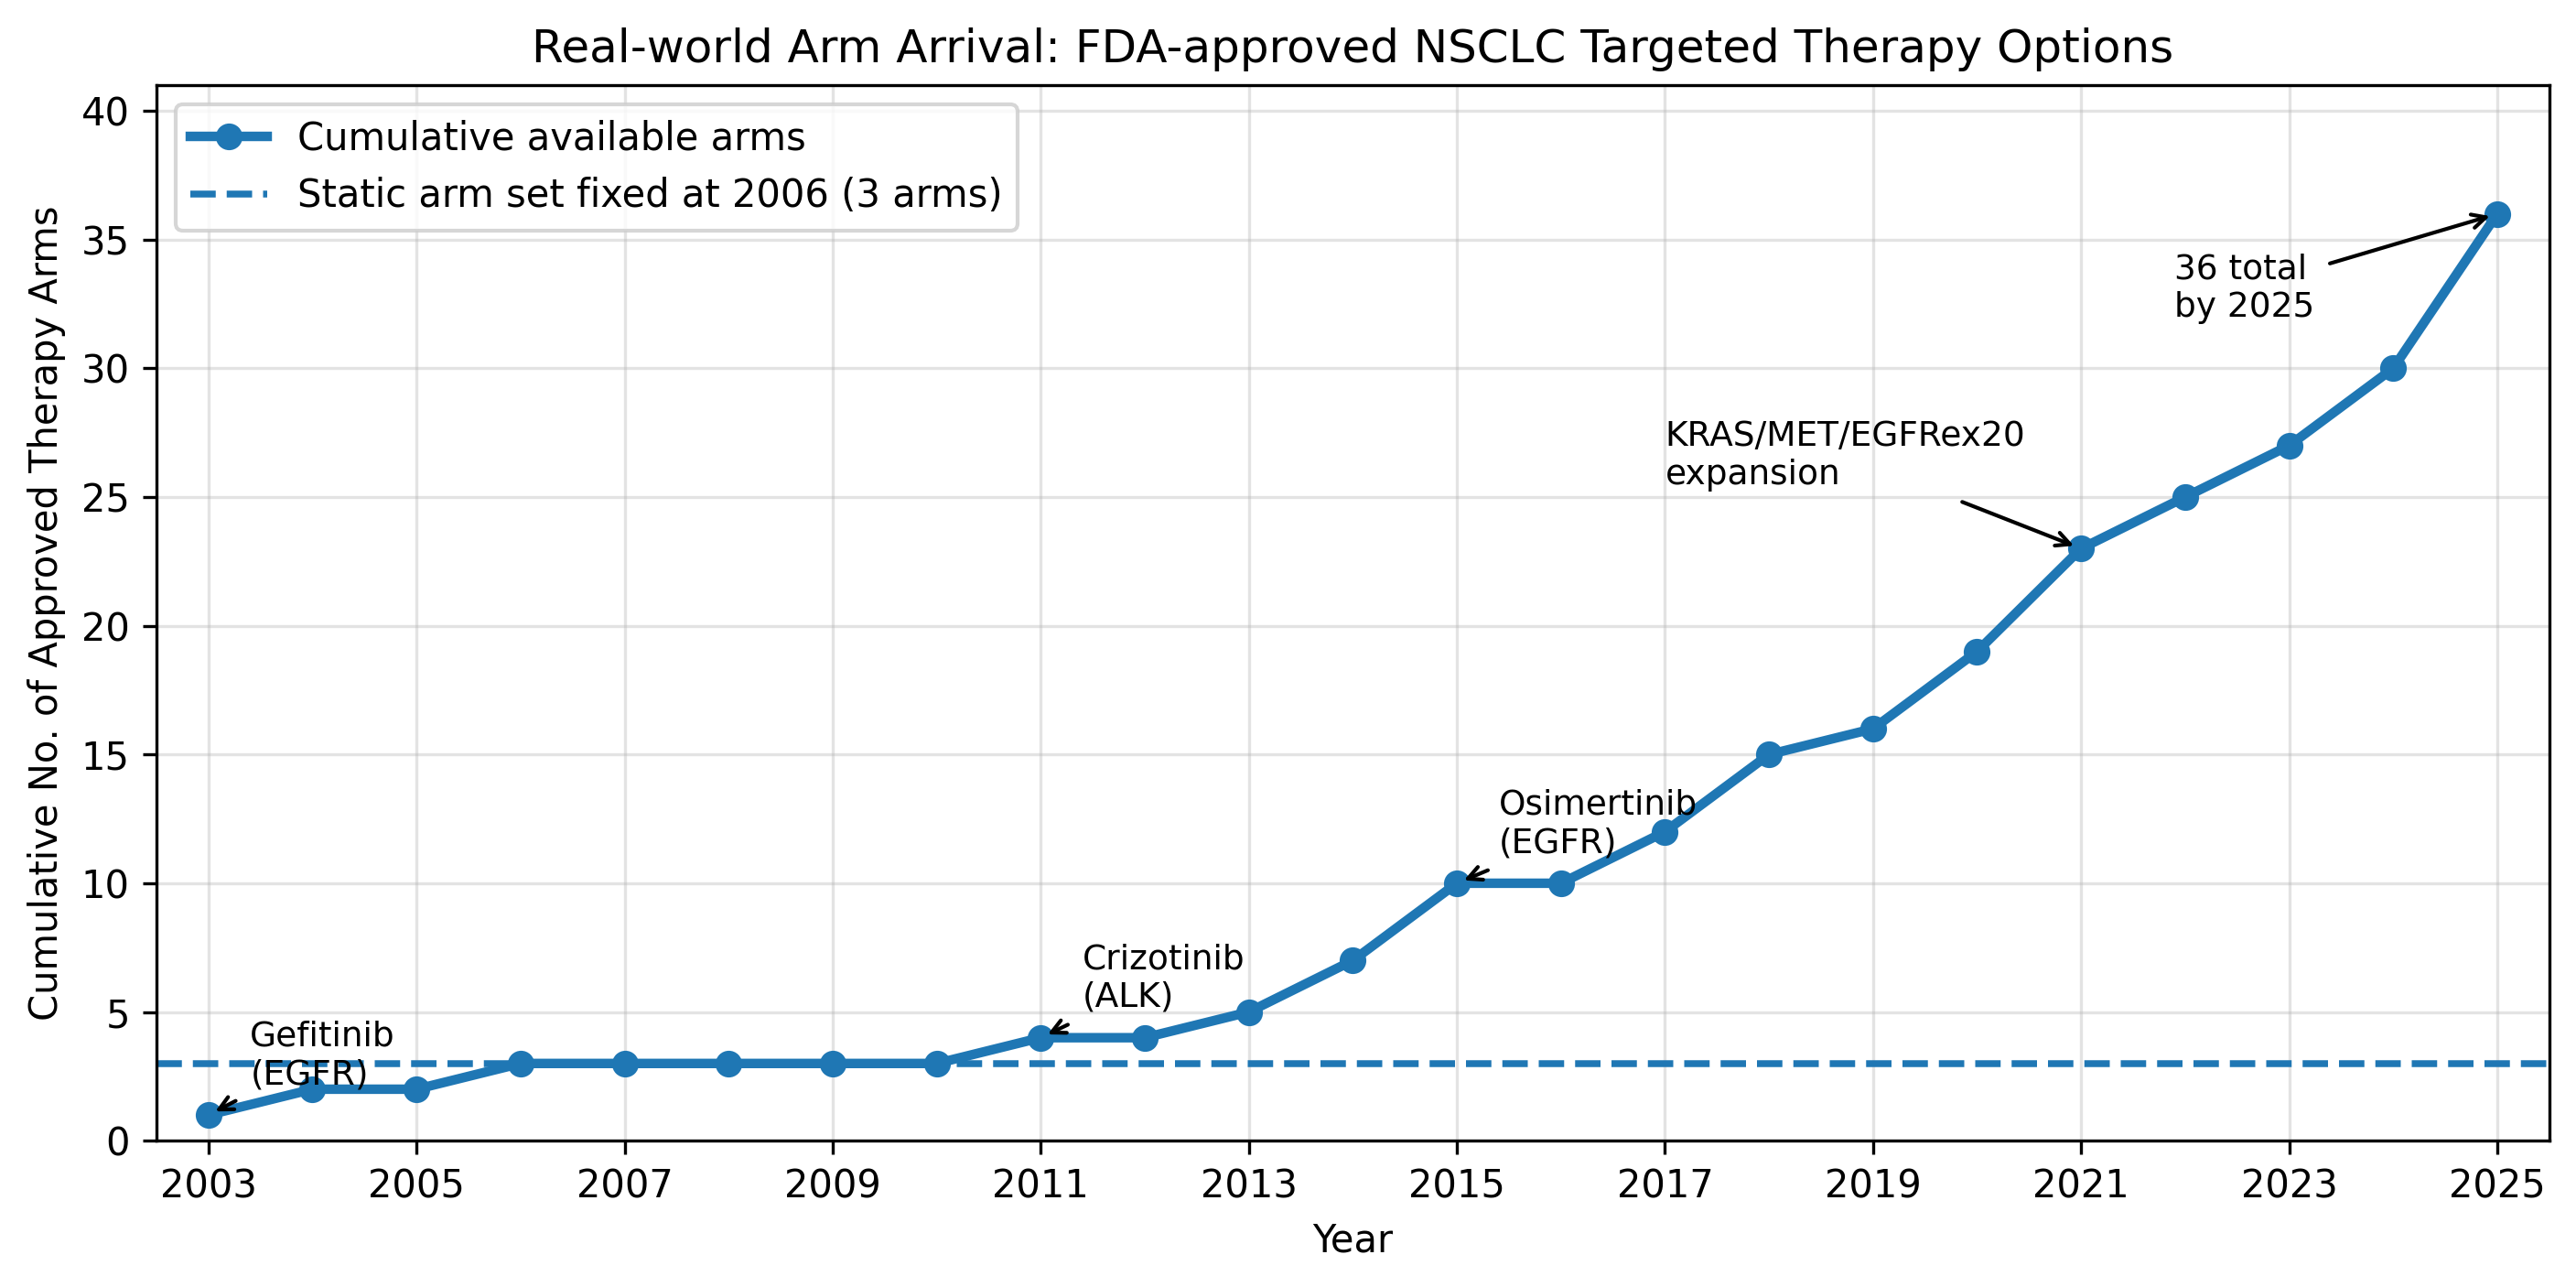
\includegraphics[width=0.9\textwidth]{figure_nsclc_targeted_therapy_arms.png}
    \caption{\textbf{The rapid expansion of the decision space in precision oncology.} FDA approval data for NSCLC (2003--2025). The solid line shows the cumulative number of targeted and immunotherapies (arms), from 1 in 2003 (Gefitinib) to 36 by 2025. A static algorithm fixed to the 2006 arm set would fail to incorporate most subsequently available treatments, illustrating the need for methods that accommodate arriving arms.}
    \label{fig:nsclc_growth}
\end{figure}

Motivated by such problems, we study the \textbf{multi-armed bandit problem with arriving arms} (MAB-AA). Let \(A_t\) denote the set of arms available at time \(t\), and suppose that \(A_t \subseteq A_{t+1}\), so that new arms arrive over time and remain available thereafter. In this setting, performance is more naturally evaluated against the best arm currently available than against the single best arm in hindsight, since the latter may not have been available earlier.

Relative to the classical stochastic bandit setting, MAB-AA introduces two main difficulties. The first is \emph{arrival information discrepancy (AID)}: newly arrived arms must be explored, which repeatedly diverts samples away from well-understood incumbent arms. The second is a \emph{drifting benchmark (DB)}: as better arms enter the system, both the identity of the optimal arm and the regret benchmark may change over time.

The arriving-arm setting is related to, but distinct from, several existing bandit formulations. Unlike infinite-armed bandits \parencite{10.1214/aos/1069362389}, where arms are actively sampled from a reservoir, new arms here arrive exogenously and remain available thereafter. Unlike mortal bandits \parencite{NIPS2008_788d9869}, the defining feature is not arm death, and unlike sleeping bandits \parencite{10.1007/s10994-010-5178-7}, the available set evolves monotonically over time. Our setting is also related to bandits with moving comparators: in nonstationary and switching bandits, the best arm may change because reward distributions vary over time \parencite{Besbes2014,Auer2019ADSWITCH}, whereas in MAB-AA each arm has a stationary reward law after arrival and benchmark changes are driven only by the exogenous arrival of new arms. 

Most closely related, \textcite{ghalme2021ballooning} studies ballooning bandits with regret measured against the best currently available arm, but focuses on feasibility of sublinear regret under restricted arrival patterns. Relatedly, \textcite{qi2025graphfeedback} considers an expanding-arm extension in graph-feedback bandits with similar arms. In contrast, our focus is the unstructured arriving-arm case, which is more suitable in applications where new options are introduced over time, previously introduced options remain available, and reliable similarity or contextual structure across options is unavailable. Examples include online product or content recommendation with continuously added items, adaptive A/B testing with newly launched treatments or designs, and sequential decision problems in which candidate actions are generated by an external pipeline rather than chosen by the learner.

From a statistical perspective, multi-armed bandit problems have long been studied as models for sequential allocation and adaptive experimentation, dating back to \textcite{Robbins1952} and the asymptotically efficient allocation theory of \textcite{LAI19854}; see also \textcite{Lai1987} for connections to adaptive treatment allocation. This viewpoint has motivated a broad statistical literature, including Bayesian and index-based approaches to sequential allocation \parencite{Gittins1979,BerryFristedt1985}, response-adaptive randomization in clinical trials \parencite{Zelen1969,WeiDurham1978,VillarBowdenWason2015,WilliamsonVillar2020,AzizKaufmannRiviere2021}, covariate-dependent and nonparametric bandit methods \parencite{Woodroofe1979,YangZhu2002,RigolletZeevi2010,PerchetRigollet2013}, and recent high-dimensional, semiparametric, and transfer-learning formulations \parencite{QianYang2016,QianIngLiu2023,CaiCaiLi2024}. These works share with ours the broad goal of learning from accumulated evidence to reduce allocation to inferior alternatives, but they focus on a fixed set of treatments or actions, and thus are not applicable to the arising arm setting that we study.


Methodologically, the two challenges call for different but complementary design principles. To address AID, our approach combines elimination steps \parencite{EvenDar2006SE,Auer2010UCBRI,PerchetRigollet2013,QianYang2016} with a pre-elimination mechanism tailored to the expanding action set. The key idea is to prevent the main competition stage from being repeatedly disrupted by every newly arriving arm. Instead, late arrivals are first screened against incumbent candidates, so that clearly inferior arms can be removed before receiving the full exploration budget assigned to serious contenders. To handle DB, the algorithm repeatedly updates the relevant comparison set as new arms arrive, and the analysis evaluates regret against the best arm currently available rather than against a fixed hindsight oracle. 

Based on these ideas, we propose \textbf{UCB for Arriving Arms (UCB-AA)}. For UCB-AA, we derive regret upper bounds that depend explicitly on the arrival process, establish sublinear dynamic regret under suitable conditions on gap evolution, study representative lower-bound regimes, and develop an online extension for unknown horizons.

Our contributions are threefold. First, we formulate the arriving-arm stochastic bandit problem using a dynamic-regret benchmark relative to the best currently available arm. Second, we propose a screening-based elimination procedure that is tailored to the information imbalance between incumbent and newly arrived arms. Third, we provide regret guarantees, lower-bound insights in representative regimes, and an online extension, together with simulations showing that UCB-AA reduces wasted pulls and maintains a compact active arm set.

The remainder of the paper is organized as follows. Section~\ref{sec:problem} formulates the problem and introduces the regret criterion. Section~\ref{sec:algorithm} presents UCB-AA, its theoretical guarantees, and an online extension for unknown horizons. Section~\ref{sec:lowerbound} develops lower bounds in representative regimes. Section~\ref{sec: simulation} reports numerical results. Section~\ref{sec:Discussion} concludes.

\section{Multi-Armed Bandit Problem with Arriving Arms }
\label{sec:problem}


\subsection{Problem Formulation}

We consider a sequential decision process over time steps $t = 1, 2, \dots$. Let $\mathcal{A}$ denote the (possibly infinite) set of all arms. At each time step $t$, only a subset $\mathcal{A}_t \subset \mathcal{A}$ is available, and we assume that the available set is non-decreasing:
$\mathcal{A}_t \subseteq \mathcal{A}_{t+1}.$
For any arm $i \in \mathcal{A}$, define its arrival time as
$\tau_i := \inf\{t\ge 1: i \in \mathcal{A}_t\}$.
Each arm $i$ is associated with an unknown reward distribution on $[0,1]$ with mean $r_i$. When arm $i$ is pulled at time $t$, a reward $X_{t,i}$ is generated; for each fixed $i$, we assume $\{X_{t,i}\}_{t\ge 1}$ are i.i.d. with mean $r_i$, and rewards are independent across arms. The arrival process is treated as exogenous to the learner.

A policy is a sequence $\pi = (\pi_t)_{t\ge 1}$, where each decision rule $\pi_t$ maps the past history to an available arm $I_t := \pi_t(H_{t-1}) \in \mathcal{A}_t,$ where $H_{t-1} := \big(\mathcal{A}_s, I_s, X_{s,I_s}\big)_{s=1}^{t-1}$
denote the observed history up to time $t-1$. Then the learner observes only $X_{t,I_t}$. Because the available set changes over time, the best arm may also change. We define the best mean reward at time $t$ as
$r^*(t) := \max_{i \in \mathcal{A}_t} r_i.$

For any (possibly random) stopping time $\tau$, define the cumulative regret by the (expected) regret against the best available arm at each time:
\[
R_{\tau}(\pi):=\sum_{t=1}^{\tau}\bigl(r^*(t)-r_{I_t}\bigr).
\]
For a deterministic horizon $T$, this reduces to $R_T(\pi)$. For the round-based procedure analyzed below,
the relevant stopping time is $T_0(\pi)$, the total number of pulls used to complete $M$
rounds. 
This benchmark differs from the usual regret against the single best arm in hindsight. In the arriving-arm setting, the terminal best arm in \(\mathcal{A}_T\) may not have been available in earlier periods, so comparing the learner with that arm throughout the entire horizon may overstate the achievable performance. The criterion above instead compares the learner at each time \(t\) with the best arm that was actually available at that time. When \(\mathcal{A}_t\) is constant over time, this formulation reduces to the classical stochastic multi-armed bandit problem.

\subsection{Main Statistical Challenges}
Relative to the classical fixed-arm stochastic bandit model, the arriving-arm setting introduces two related sources of difficulty.

\textbf{Arrival Information Discrepancy (AID):}
A first difficulty is arrival information discrepancy. With a finite sampling budget up to time $T$, the learner must allocate samples both to incumbent arms and to newly arriving arms whose rewards are still highly uncertain. Under continual arrivals, this repeated re-exploration can prevent the learner from concentrating pulls on the best currently available arm. Consequently, without additional regularity conditions on the arrival process, sublinear regret may be unattainable.

\textbf{Drifting Benchmark (DB):}
In contrast to the classical setting where the best mean reward is fixed, the benchmark in MAB-AA is time-dependent: $r^*(t)=\max_{i\in \mathcal{A}_t} r_i$. Since $\mathcal{A}_t$ expands over time, both the identity of the best arm and the value $r^*(t)$ may change when new arms arrive. Consequently, for a fixed arm $i$, the suboptimal gap $r^*(t)-r_i$ is generally time-varying (and non-decreasing in $t$). This drifting benchmark complicates both algorithm design and analysis, because the learner must continuously compare well-sampled incumbent arms with newly arriving arms whose estimates are still highly uncertain.


\section{UCB for Arriving Arms (UCB-AA) Algorithm}
\label{sec:algorithm}



\subsection{Algorithm Description}



UCB-AA is an elimination-based procedure organized by rounds. Its main idea is simple:
newly arriving arms are not allowed to compete immediately with well-sampled incumbent
arms. Instead, they are first buffered and screened at lower cost. Only those that survive
this screening step enter full competition in the next stage. This design aims to reduce
wasted exploration on clearly suboptimal late arrivals while preserving the ability to detect
genuinely competitive new arms.

Fix a finite number of rounds \(M\). For each round \(m=0,1,\dots,M\), let \(A_m\) denote
the set of arms arriving during round \(m-1\), with \(A_0\) the initial arm set, and define
\(
A(m):=\bigcup_{j=0}^m A_j .
\)
Let \(C_m\) denote the set of arms surviving round \(m\). Then round \(m\) starts from the
surviving incumbent arms \(C_{m-1}\) together with the newly admitted batch \(A_m\).
We write \(B_m\) for the active set in that round.

We assume that the cumulative number of arrived arms is bounded by a known nondecreasing
function \(K(m)\):
\[
|A(m)| \le K(m), \qquad |A_{m+1}| \le K(m+1)-K(m).
\]
For simplicity, assume that the best arm is unique in each round. Let
\(
r_{*(m)}:=\max_{i\in B_m} r_i,
\)
and let \(*(m)\in B_m\) denote the corresponding optimal arm. For each arm \(i\), define
its arrival round $t_i:=\min\{m:i\in A_m\}$, and its round-\(m\) suboptimality gap
\[
\Delta_i(m):=
\begin{cases}
r_{*(m)}-r_i, & m\ge t_i,\\
0, & m<t_i.
\end{cases}
\]




In round $m$, UCB-AA proceeds in two stages. As shown in Algorithm~\ref{alg:ucb-aa}, the earlier phases $p=0,\ldots,m-2$ are used for pre-elimination of newly arrived arms, while the last two phases $p=m-1,m$ are used for elimination on the merged active set. 


\begin{algorithm}[H]
\caption{\textbf{UCB for Arriving Arms (UCB-AA)}}
\label{alg:ucb-aa}
\small
\begin{algorithmic}[1]
\Require number of rounds $M$, parameter $N>0$.
\State \textbf{Initialization:} $\tilde{\Delta}_0 \coloneqq 1$, $B_{-1} \coloneqq \varnothing$, $C_{-1} \coloneqq \varnothing$, $T_0 \gets 0$.

\Procedure{Elim}{$S,\;R,\;p$}
    \State $n_p \coloneqq \left\lceil \frac{2\log(N\tilde{\Delta}_p^2)}{\tilde{\Delta}_p^2} \right\rceil$
    \State Pull each $j\in S$ to $n_p$ total pulls; update $T_0$ after each pull
    \State Let $b_p\coloneqq\sqrt{\frac{\log(N\tilde{\Delta}_p^2)}{2n_p}}$; set $\mathrm{LCB}_j=\hat r_j(n_p)-b_p$, $\mathrm{UCB}_j=\hat r_j(n_p)+b_p$
    \State Remove from $S$ any $j$ with $\mathrm{UCB}_j \le \max\limits_{i\in R}\mathrm{LCB}_i$
    \State \Return $S$
\EndProcedure

\For{$m=0,1,\dots,M$}
    \State Receive $A_m$ and set $B_m^0 \coloneqq C_{m-1}\cup A_m$

    \If{$|A_m|\neq 0$ and $m\ge 2$}
        \State $A_m^0 \coloneqq A_m$
        \For{$p=0,1,\dots,m-2$}
            \State $A_m^{p+1} \gets$ \Call{Elim}{$A_m^p,\;B_m^p,\;p$}; $B_m^{p+1} \coloneqq C_{m-1}\cup A_m^{p+1}$
        \EndFor
    \EndIf

    \If{$m=0$}
        \State $B_m^{1} \gets$ \Call{Elim}{$B_m^0,\;B_m^0,\;0$}
    \Else
        \For{$p=m-1,m$}
            \State $B_m^{p+1} \gets$ \Call{Elim}{$B_m^p,\;B_m^p,\;p$}
        \EndFor
    \EndIf
    \State $C_m \coloneqq B_m^{m+1},\; \tilde{\Delta}_{m+1}=\frac{1}{2}\tilde{\Delta}_{m}$
\EndFor
\end{algorithmic}
\end{algorithm}

\subsubsection{Stage I: Pre-elimination of newly arrived arms}

At the beginning of round \(m\), the newly admitted batch \(A_m\) is screened
against the surviving incumbent set \(C_{m-1}\). During the preliminary phases
\(p=0,\ldots,m-2\), only arms in \(A_m\) are subject to removal: each surviving
new arm is sampled to the phase-specific target \(n_p\), and is discarded if its
upper confidence bound falls below the largest lower confidence bound of the
reference set.
This stage exploits the information asymmetry between incumbents and arrivals.
Incumbent arms have typically accumulated more samples, whereas newly arrived
arms are still highly uncertain. Screening arrivals before full competition
therefore prevents clearly inferior late arrivals from consuming the exploration
budget assigned to serious contenders.

\subsubsection{Stage II: Formal elimination on the active set}

After pre-elimination, the surviving new arms are merged with the incumbent arms to form
the active set for round \(m\). UCB-AA then applies elimination to the full active set.
At this stage, both incumbent and newly arrived arms may be removed. The surviving set is
denoted by \(C_m\) and is carried into the next round. Thus, unlike a naive elimination rule, UCB-AA does not allow newly arrived arms to enter the main elimination stage immediately upon arrival. They must first pass the preliminary screening step in phases $p=0,\ldots,m-2$. Once merged into the active set, however, all surviving arms are handled in the same way.


\subsection{Regret Decomposition}
\label{sec: Regret Decomposition}
Our analysis is indexed by the number of rounds \(M\), rather than by fixing the total
number of pulls in advance. We assume that the sampling budget is sufficient for UCB-AA
to complete all \(M\) rounds, so the total number of pulls used up to the end of round \(M\)
is a policy-dependent random variable. For a policy \(\pi\), let \(T_0(\pi)\) denote this total,
and write
\[
T:=\mathbb{E}[T_0(\pi)].
\]
Let \(N^\pi_{i,m}\) be the number of times arm \(i\) is
pulled during round \(m\). Then \(
T_0(\pi)=\sum_{m=0}^M \sum_{i\in B_m} N^\pi_{i,m},\)
where \(B_m\) is the active set at the beginning of round \(m\).

Because UCB-AA updates its active set only at round boundaries, it is convenient to first
analyze regret against the benchmark fixed at the beginning of each round. Define the
\emph{roundwise regret}
\[
R_M(\pi):=\sum_{m=0}^M \sum_{i\in B_m} N^\pi_{i,m}\Delta_i(m).
\]
This quantity charges each pull in round \(m\) against the best arm in the active set at the
start of that round.
Our target criterion, however, is the original dynamic regret
\[
R_{T_0}(\pi)=\sum_{t=1}^{T_0(\pi)}\bigl(r^*(t)-r_{I_t}\bigr),
\]
where \(r^*(t)=\max_{i\in A_t} r_i\) is the best mean reward among all arms available at
time \(t\). These two regret notions differ because a benchmark-improving arm may arrive
within a round but is not incorporated into the active set until the next round.

Accordingly, we decompose the dynamic regret as
\(
R_{T_0}(\pi)=R_M(\pi)+D_M(\pi),
\)
where
\[
D_M(\pi):=R_{T_0}(\pi)-R_M(\pi)
\]
is the \emph{delay regret}. The term \(R_M(\pi)\) captures the main statistical cost of
identifying competitive arms under the round structure, while \(D_M(\pi)\) captures the
additional loss caused by delayed incorporation of within-round benchmark improvements.
The remainder of this section controls these two terms separately: we first bound the
roundwise regret \(R_M(\pi)\), and then bound the delay regret \(D_M(\pi)\).

\subsection{Upper Bound for the Roundwise Regret}\label{sec: Upper Bound for the Roundwise Regret}

We now bound the principal term in the decomposition of Section 3.2.
The main question is how much regret is incurred before a suboptimal arm is removed under
the elimination schedule of UCB-AA.
To formalize this, define
\[
m_i:=\min\Bigl\{m\in\{t_i,t_i+1,\dots,M\}:\tilde\Delta_m<\tfrac12\Delta_i(m)\Bigr\},
\]
the first round in which arm \(i\) becomes statistically eliminable under the target
resolution sequence. Also define
\[
\tilde m_i:=\min\Bigl\{m\in\{0,1,\dots,M\}:\tilde\Delta_m<\tfrac12\Delta_i(m_i)\Bigr\},
\]
so that \(\tilde m_i\le m_i\).
We classify suboptimal arms according to the phase in which they are eliminated with high
probability:
\begin{itemize}
    \item \(G_1\) ($m_i=t_i$): arms eliminated when they first appear;
    \item \(G_2\) ($m_i>t_i,\;\tilde{m}_i=m_i$): arms are eliminated in the formal elimination phase \(p=m_i\) of round \(m_i\);
    \item \(G_3\) ($m_i>t_i,\;\tilde{m}_i<m_i$): arms are eliminated in the formal elimination phase \(p=m_i-1\) of round \(m_i\).
\end{itemize}

For a threshold \(\lambda \ge 2^{-M+1}\), define
\(
A'(\lambda):=\{i\in A(M):\Delta_i(M)>\lambda\}.
\)
Then \(A'(\lambda)\) admits the partition
\(
A'(\lambda)=G_1(\lambda)\cup G_2(\lambda)\cup G_3(\lambda).
\)
Moreover, define
\[
\bar m_i:=
\begin{cases}
\tilde m_i, & i\in G_1(\lambda)\cup G_2(\lambda),\\
m_i-1, & i\in G_3(\lambda).
\end{cases}
\]
Thus \(\bar m_i\) is the elimination scale at which arm \(i\) is removed with high probability.

\begin{theorem}[Upper bound for the roundwise regret]
\label{thm:ucb-aa-upper}
For any $\lambda\geq 2^{-M+1}$, the regret of UCB-AA up to round $M$ satisfies
\begin{align*}
\mathbb{E}R_M(\pi)
\leq
\sum_{\substack{i: \Delta_i(M) \geq \lambda}}
\left(
\tilde{S}_i
+
\frac{4\bigl(K(m_i)+5\bigr)\,R_i}{N\tilde{\Delta}_{\tilde{m}_i}^2}
\right)
+
T\max_{i:\Delta_i(M)\leq \lambda}\Delta_i(M),
\end{align*}
where $T = \mathbb{E}[T_0(\pi)]$ denotes the expected total number of pulls,
\[
R_i\coloneqq n_{t_i}\Delta_i(t_i)+\sum_{m=t_i+1}^M\bigl(n_m-n_{m-1}\bigr)\Delta_i(m),
\]
and
\[
\tilde{S}_i\coloneqq
\begin{cases}
    n_{\tilde{m}_i}\,\Delta_i(t_i), & i\in G_1(\lambda),\\
    n_{t_i}\Delta_i(t_i)+\sum_{m=t_i+1}^{\overline{m}_i}\bigl(n_m-n_{m-1}\bigr)\Delta_i(m), & i\in G_2(\lambda)\cup G_3(\lambda).
\end{cases}
\]
\end{theorem}

Theorem~\ref{thm:ucb-aa-upper} decomposes the roundwise regret into three statistically interpretable components. The leading term, \(\tilde S_i\), is the identification cost of certifying that a suboptimal arm should be removed at the resolution dictated by the elimination schedule. The second term quantifies the additional regret incurred on low-probability events where statistical fluctuations delay elimination or allow an incorrect survivor to persist. The final truncation term collects arms whose terminal gaps are below the target resolution \(\lambda\), and may therefore be treated as effectively indistinguishable at the scale of the analysis.

To obtain a simpler rate statement, we impose the following stability condition.

\begin{assumption}[Gap stability]
\label{ass:gap_stability}
For every suboptimal arm \(i \in A'(\lambda)\), there exists a universal constant \(\tilde{C}>0\), independent of \(\lambda\), such that
\[
\Delta_i(M) \leq \tilde{C}\,\Delta_i(m_i).
\]
\end{assumption}

Assumption~\ref{ass:gap_stability} does not restrict the arrival times of arms;
rather, it limits how much the benchmark can improve after an arm has already
become statistically distinguishable. Equivalently, the post-detection benchmark
increase cannot be larger than a constant multiple of the gap already visible at
\(m_i\).
This is a mild condition in several common regimes. It holds with
\(\tilde C=1\) if the best arm available at the terminal round has already
arrived by \(m_i\), or more generally if no later arrival improves the benchmark.
It also holds whenever later improvements are moderate relative to the current
detectable gap, for example if
\(
r_{*(M)}-r_{*(m_i)}\le c\,\Delta_i(m_i)
\)
for a constant \(c\), in which case \(\tilde C=1+c\). This covers environments
with bounded multiplicative benchmark growth after detection, as well as
settings in which only a finite number of post-detection benchmark-improving
arrivals occur and their cumulative improvement is comparable to the detection
scale. Another simple case is a separated-gap regime: if every arm in
\(A'(\lambda)\) has \(\Delta_i(m_i)\ge \delta_0>0\) for a fixed \(\delta_0\),
then bounded rewards imply \(\Delta_i(M)\le 1\le \delta_0^{-1}\Delta_i(m_i)\).
Thus the assumption mainly rules out extreme post-detection drift, where an arm
is already clearly inferior but many substantially better arms arrive later and
inflate its terminal gap by an unbounded factor.


\begin{corollary}
\label{cor:ucb_aa_simplified}
Suppose that Assumption~\ref{ass:gap_stability} holds for all $i\in A'(\lambda)=\{i\in A(M):\Delta_i(M)>\lambda\}$. Let $K\coloneqq K(M)$ and choose
\[
N = 10K\,n_M,
\qquad
\lambda \asymp \sqrt{\frac{K\log K+K}{T}}.
\]
Then the roundwise regret of UCB-AA satisfies
\[
\mathbb{E}R_M(\pi)\lesssim \sqrt{K\log K\cdot T}.
\]
\end{corollary}

Corollary~\ref{cor:ucb_aa_simplified} shows that UCB-AA achieves sublinear roundwise regret when the effective
number of arriving competitors remains moderate relative to the available sample size.
Here \(K=K(M)\) is the cumulative number of arms that may have appeared by round \(M\),
rather than the total size of the global arm universe. In particular, the bound is informative
in regimes where \(
K(M)=o\left(\frac{T}{\log T}\right),
\)
so that the AID effect created by continual arrivals remains controllable.

\begin{note}
The parameter \(N\) must be fixed before running UCB-AA. In the theoretical analysis,
we use the conservative calibration
\(
N=10K(M)n_M, 
\;\;
n_M=\left\lceil 
\frac{2\log(N\widetilde\Delta_M^2)}{\widetilde\Delta_M^2}
\right\rceil ,
\)
where \(K(M)\) is a prior upper bound on the cumulative number of arrived arms. Although
this implicit relation can be solved approximately, its role is mainly analytical: it ensures
uniform control of low-probability failure events over all arms, but may lead to overly large
pull targets \(n_m\), and hence excessive forced exploration in both the pre-elimination and
formal elimination stages. For implementation, we use a less conservative calibration based only on the monotonicity
of the target sequence \(\{n_m\}_{m=0}^M\). Since
\(
f(x)=\frac{\log(Nx)}{x}
\)
is decreasing on \([\widetilde\Delta_M^2,1]\) whenever
\(N\widetilde\Delta_M^2\ge e\), a natural lower-end choice is
\(
N_{\min}=\frac{e}{\widetilde\Delta_M^2}.
\)
This optimistic calibration is not used in the regret proof, but provides a practical baseline
with substantially smaller pull targets, and is adopted in the simulations.

\end{note}

\subsection{Control of the Delay Regret}

Delay regret arises because UCB-AA updates its active set only at round boundaries. If a
benchmark-improving arm arrives in the middle of round \(k\), then the true dynamic
benchmark improves immediately on the original timeline, whereas the roundwise benchmark
used in \(R_M(\pi)\) is updated only at the beginning of round \(k+1\). Thus \(D_M(\pi)\)
captures the additional loss caused by this deferred incorporation of within-round benchmark
improvements.

Fix a round \(k\). Suppose that within this round there are \(q_k\) benchmark-improving
arrival events, with increments
\[
\beta_{k,1},\dots,\beta_{k,q_k}\ge 0,
\qquad 
\sum_{j=1}^{q_k}\beta_{k,j}=: \delta_k,
\]
where
\(
\delta_k=r_{*(k+1)}-r_{*(k)}
\)
is the total benchmark increase associated with round \(k\). Let \(L_k\) be the total number
of pulls in round \(k\), and let
\(
1\le \tau_{k,1}<\cdots<\tau_{k,q_k}\le L_k
\)
denote the within-round locations of these improving arrivals. We define the exposure factor
\[
\rho_k:=
\frac{1}{L_k\delta_k}
\sum_{j=1}^{q_k}(L_k-\tau_{k,j}+1)\beta_{k,j},
\qquad \delta_k>0,
\]
so that \(0\le \rho_k\le 1\). The factor \(\rho_k\) measures how much of round \(k\) is exposed
to the benchmark increase: improvements that occur early contribute more to delay regret than
those that occur late.
For \(\ell\ge k+1\), define the cumulative benchmark improvement after round \(k\) by
\[
\Delta_{*(k)}(\ell):=r_{*(\ell)}-r_{*(k)}=\sum_{i=k}^{\ell-1}\delta_i.
\]
We also define
\(
m_{*(k)}=\min\Bigl\{\ell\ge k+1:\tilde\Delta_\ell<\tfrac12\Delta_{*(k)}(\ell)\Bigr\},
\)
the first round at which the cumulative improvement after round \(k\) becomes statistically
detectable under the elimination schedule.

\begin{note}
For analytical convenience, we take the analyzed horizon to end at a checkpoint immediately
after the last batch of arrivals has been admitted. Equivalently, one may append a terminal
bookkeeping round with no further sampling. This convention does not require the learner to
determine whether the final arrivals improve the benchmark; it only ensures that no arrivals
remain unincorporated at the endpoint. Under this convention, the terminal delay contribution
is null, so the endpoint condition involving \(\rho_M\delta_M\) becomes vacuous.
\end{note}

To bound \(D_M(\pi)\), we impose a condition that limits how aggressively benchmark
improvements can accumulate before they become statistically detectable. This condition is
used to close the upper bound and should be viewed as a sufficient condition, not a necessary
one.

\begin{assumption}[Cumulative jump control]\label{ass:delay_cum}
Assume that for every round $k$ satisfying $\rho_k\delta_k>\lambda$, one has $m_{*(k)}>k+1$,
and at least one of the following conditions holds:
\begin{align}
\Delta_{*(k)}\bigl(m_{*(k)}\bigr)
&\le
\tilde{\Delta}_k
\sqrt{
\frac{M-m_{*(k)}+1}{3\rho_k K(k)(M-k+1)}
},
\label{eq:delay-cond-1}
\\
\frac{\delta_k}{\Delta_{*(k)}(m_{*(k)}-1)}
&\le
\frac{2^{\,m_{*(k)}-k-2}}{\rho_k K(k)}.
\label{eq:delay-cond-2}
\end{align}
\end{assumption}
Assumption~\ref{ass:delay_cum} is most naturally satisfied when benchmark improvements remain moderate until
they become detectable at the current resolution scale. This includes, for example, settings in
which improvements occur gradually, settings in which large improvements are rare, or settings
in which most benchmark-improving arrivals occur late within a round and therefore have
small exposure factors \(\rho_k\).

\begin{proposition}[Delay regret under cumulative jump control]\label{prop:delay_cum}
Let
\(
\lambda\ge 2^{-M+1}.
\)
Under Assumption~\ref{ass:delay_cum},
\[
\mathbb{E}\bigl[D_M(\pi)\bigr]
\le
\sum_{i:\Delta_i(M)>\lambda}\tilde S_i+\lambda T.
\]
\end{proposition}

Proposition \ref{prop:delay_cum} shows that, under cumulative control of benchmark jumps, the delay regret is bounded by the same certification-type quantity that appears in the main regret analysis, up to the truncation term $\lambda T$. Hence the delayed admission of within-round arrivals does not create a new leading-order source of statistical difficulty. More broadly, the result clarifies how the dynamic benchmark enters the regret analysis: the regret of MAB-AA can be viewed as consisting of a principal identification term and an additional delay term induced by benchmark improvement. Under Assumption~\ref{ass:delay_cum}, the latter remains controlled, so benchmark movement acts as a structured perturbation of the elimination problem rather than as a fundamentally separate source of regret.


\subsection{General regret bound}

We now return to the original dynamic regret
\(
R_{T_0}(\pi)
=
\sum_{t=1}^{T_0(\pi)}\bigl(r^*(t)-r_{I_t}\bigr).
\)
By the decomposition in Section~\ref{sec: Regret Decomposition},
\[
R_{T_0}(\pi)=R_M(\pi)+D_M(\pi).
\]
Theorem~\ref{thm:ucb-aa-upper} controls the principal term \(R_M(\pi)\), and Proposition~\ref{prop:delay_cum} controls the delay term \(D_M(\pi)\). Combining the two results yields the following bound for the original regret criterion.

\begin{theorem}[General regret bound]
\label{thm:general bound}
Let 
\(
\lambda \ge 2^{-M+1}.
\)
Suppose that Assumptions \ref{ass:gap_stability} and \ref{ass:delay_cum} hold. Then the dynamic regret of UCB-AA satisfies
\[
\mathbb{E} R_{T_0}(\pi)
\le
\sum_{i:\Delta_i(M)\ge \lambda}
\left(
2\tilde S_i+
\frac{4\bigl(K(m_i)+5\bigr)R_i}{N\tilde\Delta_{\tilde m_i}^2}
\right)
+2\lambda T .
\]
In particular, under the conservative calibration of $N$ in Corollary~\ref{cor:ucb_aa_simplified},
\[
\mathbb{E}R_{T_0}(\pi)\lesssim \sqrt{K\log K\cdot T}.
\]
\end{theorem}

\subsection{Online UCB-AA}
\label{sec:online}

We briefly discuss the case in which the terminal round \(M\) is unknown. To remove the fixed-horizon requirement, we use a geometric-restart scheme and run UCB-AA over successive stages with geometrically increasing stage lengths. This yields an anytime version of the procedure, referred to as Online UCB-AA. The idea is standard: each stage is long enough to cover the possibility that the effective horizon is of that order, and restarting across stages incurs only a logarithmic overhead relative to the fixed-\(M\) analysis. We retain the algorithm here for completeness and defer the more detailed stage-wise analysis to the Supplementary Material.

\begin{algorithm}[htbp]
\caption{Online UCB-AA}
\label{alg:online-ucb-aa}
\begin{algorithmic}[1]
\Require Base algorithm UCB-AA
\State Initialize stage index $l \leftarrow 1$
\While{interaction continues}
    \State $M_l\leftarrow2^l$, $\tilde{M}_l\leftarrow\sum_{i=1}^l M_i$, $\tilde{\Delta}_{M_l}\leftarrow2^{-M_l}$
    \State $n_{M_l}(N_l)\coloneqq\left\lceil\frac{2\log(N_l\tilde{\Delta}_{M_l}^2)}{\tilde{\Delta}_{M_l}^2}\right\rceil$
    \State Compute $N_l$ from $N_l=10K(\tilde{M}_l)n_{M_l}(N_l)$ (approx.)
    \State Run UCB-AA$(M_l,N_l)$ for $M_l$ rounds
    \State $l \leftarrow l+1$
\EndWhile
\end{algorithmic}
\end{algorithm}

At each restart, Online UCB-AA reinitializes the internal state of the base
procedure for the new stage, while all pulls across stages are still counted in
the cumulative regret.
The next corollary summarizes the resulting regret guarantee in the unknown-horizon setting.

\begin{corollary}
\label{cor:online_gap_independent}
Suppose that Assumption~\ref{ass:gap_stability} holds.
The expected roundwise regret of Online UCB-AA satisfies
\[
\mathbb{E}R_M(\pi) \lesssim \sqrt{K(M)\,T\,\log T}.
\]
If a stagewise version of Assumption~\ref{ass:delay_cum} holds uniformly across the restart stages,
then
\[
\mathbb{E}R_{T_0}(\pi) \lesssim \sqrt{K(M)\,T\,\log T}.
\]
\end{corollary}

Corollary~\ref{cor:online_gap_independent} shows that the online extension preserves the same square-root-type behavior as the fixed-\(M\) procedure, at the cost of only a logarithmic overhead due to geometric restarts. Thus, lack of prior knowledge of the terminal round does not alter the qualitative statistical difficulty of the arriving-arm problem. A more detailed stage-wise bound is given in the Supplementary Material.


\section{Lower Bounds in Representative Regimes}
\label{sec:lowerbound}

As mentioned earlier, without structural restrictions on the arrival process, sublinear regret may be unattainable
\parencite{ghalme2021ballooning}. A fully general lower bound for the unrestricted arriving-arm model is therefore not our goal here. Instead, we focus on three representative regimes that isolate distinct hardness mechanisms in MAB-AA: static identification, repeated distractor certification, and near-tied benchmark updates under a drifting comparator.

The statistical hardness of MAB-AA is therefore not monolithic. In the static limit, the problem reduces to the classical identification barrier of stochastic bandits. When a globally optimal incumbent is present from the outset and all late arrivals are inferior, the dominant cost is repeated certification of distractors. When the benchmark improves through a sequence of near-tied arrivals, the difficulty becomes a succession of local tests under a drifting comparator. This section isolates these three mechanisms and relates them to the upper-bound structure in Section~\ref{sec:algorithm}.

To avoid repeating regime-specific growth conditions, we use the following scale-sensitive extension of the usual notion of uniform goodness.

\begin{definition}[Uniform goodness at scale $h(T)$]
\label{def:uniformly-good-scale}
Let $\mathcal V_T$ be a family of bandit instances indexed by $T$, and let $h(T)\to\infty$.
A sequence of policies $\{\pi^{(T)}\}_{T\ge1}$ is \emph{uniformly good on $\{\mathcal V_T\}$ at
scale $h(T)$} if, for every $a>0$,
\[
\sup_{\nu\in\mathcal V_T}\mathbb E_{\nu}[R_T(\pi^{(T)};\nu)]
=
o\bigl(h(T)^a\bigr)
\qquad\text{as }T\to\infty.
\]
\end{definition} 


 When $h(T)=T$, it reduces to the classical requirement considered in \textcite{LAI19854,BurnetasKatehakis1996}. For related information-theoretic change-of-measure techniques in best-arm
identification, see also \textcite{KaufmannCappeGarivier2016}.

\subsection{Static Reduction}



We first consider the degenerate no-arrival case. Here $h(T)=T$, so
Definition~\ref{def:uniformly-good-scale} reduces to the usual notion of uniform goodness.
The purpose of this subsection is mainly calibrational: when no new arms enter, MAB-AA
reduces to the classical stochastic bandit problem, so the arriving-arm framework should
recover the familiar logarithmic identification barrier. Accordingly, we restate a standard
lower-bound implication from the classical bandit literature
\parencite{LAI19854,BurnetasKatehakis1996} in a form adapted to our notation. This result
is included for comparison with our arriving-arm analysis, rather than as a new contribution.
To avoid unnecessary generality, we use a local formulation under a quadratic KL condition,
which is sufficient for our comparison with the upper bounds in
Section~\ref{sec:algorithm}.

Consider a static bandit family with rewards supported on $[0,1]$. Let $\nu^{(0)}$ be a baseline
instance in which arm $0$ is the unique optimal arm with mean $r^\star\in(0,1)$. For
$i=1,\dots,K$, let arm $i$ have reward law $P_i$ and mean
\(
r_i=r^\star-\Delta_i\) where \(
\Delta_i>0.
\)

\begin{theorem}[Static lower bound]
\label{thm:static-lb-local-quadratic}
Assume that for each $i=1,\dots,K$ there exists a distribution $Q_i\in\mathcal P([0,1])$ such
that
\(
\eta_i:=\mathbb E_{Q_i}[X]-r^\star>0\) and
\(
D(P_i\|Q_i)\le C_i\Delta_i^2
\)
for some finite constant $C_i>0$. Let $\nu^{(i)}$ denote the instance obtained from $\nu^{(0)}$
by replacing only the reward law of arm $i$ from $P_i$ to $Q_i$. If a policy $\pi$ is uniformly
good on the local family $\mathcal V:=\{\nu^{(0)},\nu^{(1)},\dots,\nu^{(K)}\}$, then
\[
\mathbb E_{\nu^{(0)}}[R_T(\pi;\nu^{(0)})]
\ge
c\sum_{i=1}^K \frac{\log T}{C_i\Delta_i}
\]
for all sufficiently large $T$, where $c>0$ is an absolute constant. In particular, if $\sup_{1\le i\le K} C_i\le C_\star<\infty$, then
\[
\mathbb E_{\nu^{(0)}}[R_T(\pi;\nu^{(0)})]
\ge
c\,C_\star^{-1}\sum_{i=1}^K \frac{\log T}{\Delta_i}
\]
for all sufficiently large $T$.
\end{theorem}



\begin{example}[Static specialization]
\label{exp:static}
In the absence of arrivals, UCB-AA specializes to an elimination-style stochastic bandit
procedure and achieves
\(
\tilde O\left(\sum_i \frac{\log(T\Delta_i^2)}{\Delta_i}\right)
\)
instance-dependent regret. Together with
Theorem~\ref{thm:static-lb-local-quadratic}, this shows that the arriving-arm reduction does
not sacrifice statistical efficiency in the static limit, up to logarithmic refinements.
\end{example}

\subsection{Sequential Distractors}

We next consider a regime in which a globally optimal incumbent is present from the outset,
while every newly arriving arm is suboptimal under the baseline instance. The difficulty is
therefore repeated certification: each arrival creates a local alternative under which that arm
would become optimal, so the learner must accumulate logarithmic evidence before discarding it.

For each horizon $T$, let $\nu^{(0)}$ be a baseline instance in which arm $0$ is the unique
optimal arm, available from time $1$, with mean $r^\star\in(0,1)$. Let $\mathcal I_T$ be a
collection of arriving distractor arms. For each $i\in\mathcal I_T$, suppose arm $i$ arrives at
time $\tau_i\le T$, has reward law $P_i$, and mean
\(
r_i=r^\star-\Delta_i
\) where \(
\Delta_i>0.
\)
Write
\[
H_i(T):=T-\tau_i+1,
\qquad
H_{\min}(T):=\min_{i\in\mathcal I_T}H_i(T),
\]
and assume $H_{\min}(T)\to\infty$. In this regime we evaluate uniform goodness at the effective
scale $h(T)=H_{\min}(T)$.

\begin{theorem}[Distractor lower bound under local alternatives]
\label{thm:distractor-lb-local}
Suppose that for each $i\in\mathcal I_T$ there exists a law $Q_i\in\mathcal P([0,1])$ such that
\(
\eta_i:=\mathbb E_{Q_i}[X]-r^\star>0 \) and
\(
d_i:=D(P_i\|Q_i)<\infty.
\)
Let $\nu^{(i)}$ denote the instance obtained from $\nu^{(0)}$ by replacing the reward law
of arm $i$ from $P_i$ to $Q_i$, and set
\(
\mathcal V_T:=\{\nu^{(0)}\}\cup\{\nu^{(i)}:i\in\mathcal I_T\}.
\)
Assume that, for all sufficiently large $T$,
\[
\inf_{i\in\mathcal I_T}\Delta_i\ge \underline\Delta>0,
\qquad
\inf_{i\in\mathcal I_T}\eta_i\ge \underline\eta>0,
\qquad
\sup_{i\in\mathcal I_T}d_i\le \overline d<\infty.
\]
Then any sequence $\{\pi^{(T)}\}_{T\ge1}$ uniformly good on $\mathcal V_T$ satisfies
\[
\mathbb E_{\nu^{(0)}}[R_T(\pi^{(T)};\nu^{(0)})]
\ge
c\sum_{i\in\mathcal I_T}\frac{\Delta_i}{d_i}\log H_i(T)
\ge
c\,\underline\Delta\,\overline d^{-1}\,|\mathcal I_T|\,\log H_{\min}(T)
\]
for all sufficiently large $T$, where $c>0$ is an absolute constant.
\end{theorem}

\begin{corollary}[Two canonical distractor regimes]
\label{cor:distractor-lb-regimes}
Under the assumptions of Theorem~\ref{thm:distractor-lb-local}, suppose in addition that one
of the following holds:

\smallskip
\noindent
\textup{(i) Equal-distance arrival: } each arm in $\mathcal I_T=\{1,\dots,K_T\}$ has the same arrival interval $H:=\lfloor T/K_T\rfloor$ which means $\tau_i=(i-1)H+1$,and $H$ tends to infinity.

\smallskip
\noindent
\textup{(ii) Early arrival: } there exists a fixed $\alpha\in(0,1)$ such that
\(
\tau_i\le \alpha T\)
for every \(i\in\mathcal I_T.
\)

Then
\[
\mathbb E_{\nu^{(0)}}[R_T(\pi^{(T)};\nu^{(0)})]
\ge
c\sum_{i\in\mathcal I_T}\frac{\Delta_i}{d_i}\log H_{\min}(T)
\]
for all sufficiently large $T$. In particular, if
\[
\sup_{i\in\mathcal I_T} d_i\le \overline d<\infty,
\qquad
\inf_{i\in\mathcal I_T}\Delta_i\ge \underline\Delta>0,
\qquad
|\mathcal I_T|\asymp K_T,
\]
then
\[
\mathbb E_{\nu^{(0)}}[R_T(\pi^{(T)};\nu^{(0)})]
=
\Omega\bigl(K_T\log H_{\min}(T)\bigr).
\]
\end{corollary}

The lower bound reflects a repeated certification cost: although the arriving arms are inferior in
the baseline instance, a uniformly good policy cannot ignore them, because each arrival induces
a local alternative under which that arm is optimal.

\begin{example}[Fixed-gap distractors]
\label{exp:distractors}
Consider an initial set of arms $A_0=\{*,0\}$, where arm $*$ is globally optimal with mean
$\mu_*=\tfrac34$ and arm $0$ has mean $\mu_0=\tfrac14$. For each round $m=1,\dots,M$, a
single new arm $i=m$ arrives with
\(
\mu_i=\frac12-2^{-i-2}.
\)
Let $K(m)=m+2$ denote an upper bound on the number of arms available up to round $m$.
All new arrivals are distractors: their means converge to $1/2$, while the optimal arm remains
fixed at $3/4$, so the gaps stay bounded away from zero. Applying
Theorem~\ref{thm:ucb-aa-upper} with $N=10K(M)n_M$ yields
\(
\mathbb E R_T(\pi_{\mathrm{UCB\text{-}AA}})
=
\mathbb E R_M(\pi_{\mathrm{UCB\text{-}AA}})
=
\widetilde O\bigl(K(M)\log T\bigr).
\)
\end{example}

Combined with Theorem~\ref{thm:distractor-lb-local}, this gives the comparison
\[
\widetilde O\bigl(K_T\log T\bigr)
\qquad\text{versus}\qquad
\Omega\bigl(K_T\log(T/K_T)\bigr),
\]
so in the canonical sparse-arrival regime $K_T=o(T)$ the rates agree up to logarithmic factors.
A complementary failure-mode construction showing that the absence of pre-elimination can lead
to linear regret is deferred to the Supplementary Material.

\subsection{Progressive Near-tied Arrivals}

We finally consider a regime in which the benchmark improves through a sequence of near-tied
arrivals. Unlike the distractor setting, the main difficulty is no longer certifying clearly inferior
arms, but repeatedly deciding whether a new challenger lies slightly below or slightly above the
current reference level. Because this mechanism is intrinsically local and horizon dependent, the
natural lower bound here is a finite-horizon minimax statement.

Fix a horizon $T$ and integers $K_T\ge1$, $H_1,\dots,H_{K_T}\in\mathbb N$ such that
\(
\sum_{m=1}^{K_T} H_m=T.
\)
Define checkpoints and blocks by
\[
s_0:=0,
\qquad
s_m:=\sum_{\ell=1}^m H_\ell,
\qquad
\mathcal B_m:=\{s_{m-1}+1,\dots,s_m\},
\qquad
m=1,\dots,K_T.
\]
Let $\gamma\in(0,1/2]$, and choose
\(
\theta_1,\dots,\theta_{K_T}\in(0,1),
\;
\varepsilon_1,\dots,\varepsilon_{K_T}>0
\) 
such that
\begin{align}
\theta_m-\varepsilon_m,\ \theta_m,\ \theta_m+\varepsilon_m
&\in[\gamma,1-\gamma],
\qquad m=1,\dots,K_T,
\label{eq:prog-lb-interior}
\\
\theta_{m+1}
&\ge \theta_m+\varepsilon_m,
\qquad m=1,\dots,K_T-1.
\label{eq:prog-lb-monotone}
\end{align}
For each sign vector
\(
\sigma=(\sigma_1,\dots,\sigma_{K_T})\in\{-1,+1\}^{K_T},
\)
define an arriving-arm instance $\nu_\sigma$ in which, at time $s_{m-1}+1$, two Bernoulli
arms $c_m,d_m$ arrive and remain available thereafter, with means
\(
\mu(c_m)=\theta_m\) and \(
\mu(d_m)=\theta_m+\sigma_m\varepsilon_m.
\)
Let
\(
\mathcal V_T^{\mathrm{prog}}
:=
\{\nu_\sigma:\sigma\in\{-1,+1\}^{K_T}\}.
\)

\begin{theorem}[Deterministic-checkpoint minimax lower bound]
\label{thm:prog-lb-general}
Under \eqref{eq:prog-lb-interior}--\eqref{eq:prog-lb-monotone}, every non-anticipating policy
$\pi$ satisfies
\begin{align}
\sup_{\nu\in\mathcal V_T^{\mathrm{prog}}}
\mathbb E_\nu[R_T(\pi;\nu)]
\ge
\frac12
\sum_{m=1}^{K_T}
H_m\varepsilon_m
\left(
1-
\sqrt{
\frac{2H_m\varepsilon_m^2}{\gamma(1-\gamma)}
}
\right)_+ .
    \label{eq:prog-lb-kl-simple}
\end{align}
In particular, if there exists a constant $\kappa\in(0,1/2)$ such that
\[
H_m\varepsilon_m^2
\le
\kappa\,\gamma(1-\gamma),
\qquad
m=1,\dots,K_T,
\]
\begin{align}
    \text{then}\quad \sup_{\nu\in\mathcal V_T^{\mathrm{prog}}}
\mathbb E_\nu[R_T(\pi;\nu)]
\ge
c_\kappa
\sum_{m=1}^{K_T} H_m\varepsilon_m,
\qquad
c_\kappa:=\frac12(1-\sqrt{2\kappa})>0.
\label{eq:prog-lb-clean}
\end{align}
The same lower bounds remain valid after taking $\inf_\pi$ on the left-hand side.
\end{theorem}

Each block creates a fresh one-sided local test: the learner must determine whether the new
challenger lies slightly below or slightly above the current benchmark. When
$H_m\varepsilon_m^2$ is of constant order, the resulting regret contribution is of order
$H_m\varepsilon_m$, and these local-testing costs add across blocks.

\begin{corollary}[$\sqrt{K_TT}$ lower bound under near-homogeneous local tests]
\label{cor:prog-lb-sqrtKT}
Under the assumptions of Theorem~\ref{thm:prog-lb-general}, assume in addition that there
exist constants $c_H,C_H,c_\varepsilon,C_\varepsilon>0$ and $\kappa\in(0,1/2)$ such that, for
every $m=1,\dots,K_T$,
\[
c_H\,\frac{T}{K_T}
\le
H_m
\le
C_H\,\frac{T}{K_T},
\qquad
c_\varepsilon\sqrt{\frac{K_T}{T}}
\le
\varepsilon_m
\le
C_\varepsilon\sqrt{\frac{K_T}{T}},
\]
and
\(
C_HC_\varepsilon^2\le \kappa\,\gamma(1-\gamma).
\)
Then
\[
\inf_\pi\sup_{\nu\in\mathcal V_T^{\mathrm{prog}}}
\mathbb E_\nu[R_T(\pi;\nu)]
\ge
c\,\sqrt{K_TT}
\]
for all sufficiently large $T$, where $c>0$ depends only on $c_H,c_\varepsilon,$ and $\kappa$.
\end{corollary}

Corollary~\ref{cor:prog-lb-sqrtKT} identifies the canonical square-root minimax scale in a
near-homogeneous local-testing regime. Our general upper bound in
Section~\ref{sec:algorithm} matches this dependence up to logarithmic factors. The example
below is not a literal specialization of the deterministic-checkpoint lower bound, because
UCB-AA operates with endogenous random checkpoints, but it exhibits the same qualitative
mechanism.


\begin{example}[Monotone near-tied ladder]
\label{exp:monotone-near-tied-ladder}
Fix $M\ge 5$ and define $\xi_m := \frac12 - 2^{-m-2}$ for $m=0,1,\dots,M$. At round $0$,
there is a single arm $a_0$, so that $A_0=\{a_0\}$ and $\mu(a_0)=\xi_0$. For each round
$m=1,\dots,M$, two new Bernoulli arms arrive, namely $A_m=\{c_m,d_m\}$, with means
$\mu(c_m)=\xi_{m-1}$ and $\mu(d_m)=\xi_m$. Hence the unique optimal arm in round $m$ is
$d_m$, with $r^*(m)=\xi_m$, and the cumulative number of available arms is
$K(m)=|A(m)|=2m+1$. Choosing $N=10K(M)n_M$ yields
\(
\mathbb E R_T(\pi_{\mathrm{UCB\text{-}AA}})
=
\mathbb E R_M(\pi_{\mathrm{UCB\text{-}AA}})
=
O\bigl(\sqrt{T\log K(M)}\bigr).
\)
\end{example}



Example~\ref{exp:monotone-near-tied-ladder} should be interpreted as an endogenous-checkpoint
illustration of the same local-testing mechanism. The deterministic-checkpoint lower bound gives
the canonical minimax benchmark, while the UCB-AA analysis yields the same square-root-type
behavior up to an additional logarithmic factor along its own random checkpoint schedule.

Taken together, these lower-bound examples show that MAB-AA contains several
distinct sources of statistical difficulty. They are not intended as term-by-term
converses to the upper bounds in Section~\ref{sec:algorithm}; rather, they clarify
why the analysis must separately control the costs of identifying good incumbent
arms, certifying arriving competitors, and tracking benchmark changes.


\section{Simulation}\label{sec: simulation}
We evaluate UCB-AA on two synthetic arriving-arm environments. The first
contains abrupt improvements in the best available arm, while the second
contains frequent near-optimal arrivals. Both settings use horizon \(T=60000\).
We report three metrics:
\begin{itemize}
	    \item Cumulative dynamic regret \(R_t\): measures loss relative to the best
	    currently available arm,
	    \(R_t=\sum_{s=1}^t(r^*(s)-r_{I_s})\), where
	    \(r^*(s)=\max_{i\in\mathcal A_s}r_i\) and \(I_s\) is the arm pulled at
	    time \(s\).
    \item Wasted pulls \(W_T\): measures exploration spent on clearly suboptimal
    choices,
    \(W_T=\sum_{s=1}^T\mathbb I\{\Delta_{I_s}(s)\ge0.1\}\).
    \item Active-set size: measures the pruning effect of elimination, defined
    as the number of arms retained after elimination steps.
\end{itemize}

We consider two distinct arrival scenarios designed to stress-test different challenges inherent to the MAB-AA setting; for specific distribution parameter settings, refer to the supplementary materials: 
\subsection*{Scenario 1 (Progressive Step-up Arrivals)}
The environment starts with \(K_0=10\) arms and background arrivals following a
Poisson process with rate \(\lambda=1/200\), with means drawn from a bi-modal
mixture. To create benchmark shifts, high-performing step arms are introduced at
\(t/T\in\{0.3,0.6,0.9\}\), with
\(\mu_k=\min(1,r_0+k\Delta_{\mathrm{step}})\), \(r_0=0.6\), and
\(\Delta_{\mathrm{step}}=0.05\). This setting tests whether an algorithm can
quickly detect and switch to newly arrived superior arms.


\subsection*{Scenario 2 (Near-tied Top Set)}
The environment starts with \(K_0=20\) arms, including \(m_0=5\) near-optimal
arms with means from \(\mathrm{Uniform}(0.7,0.8)\). New arms arrive according
to a Bernoulli process with probability \(\lambda=1/200\), and \(30\%\) of them
are near-optimal. This setting represents mature decision problems with many
near-tied top arms, where small performance differences must be detected without
excessive exploration.


To ensure a fair comparison, we adapt classical algorithms to handle the continuous arrival of new arms. Their implementations are described below; additional details are provided in the supplementary materials.
\begin{enumerate}

     \item UCB-AA (Proposed): the proposed method, which buffers newly arrived
     arms and screens them through pre-elimination before full competition. We
     set \(N=e/\tilde{\Delta}_M^2\) in the simulations.
    \item Growing UCB1 (G-UCB1): UCB1 \parencite{Auer2002FinitetimeAO} with
    immediate admission of new arms, using index
    \(\hat{\mu}_{i,n}+\sqrt{2\ln t/n}\).
    \item Growing MOSS (G-MOSS): MOSS \parencite{audibert2009minimax} with
    immediate admission of new arms, using index
    \(\hat{\mu}_i+\sqrt{\max\{0,\log(T/(K_t n_i))\}/n_i}\), where
    \(K_t=|\mathcal A_t|\).

\item Dynamic Successive Elimination (D-SE): an SE-style baseline
\parencite{PerchetRigollet2013} that admits new arms at each round, samples them
to match incumbent pull counts, and then applies the SE elimination rule.

\item Naive Elimination (NE): UCB-AA with the same formal elimination rule but
without the pre-elimination stage.


\end{enumerate}


For each scenario, we ran 100 independent simulations. The figures below report
the average cumulative dynamic regret and wasted pulls, with 95\% confidence
intervals.

\begin{figure}[htbp]
    \centering
    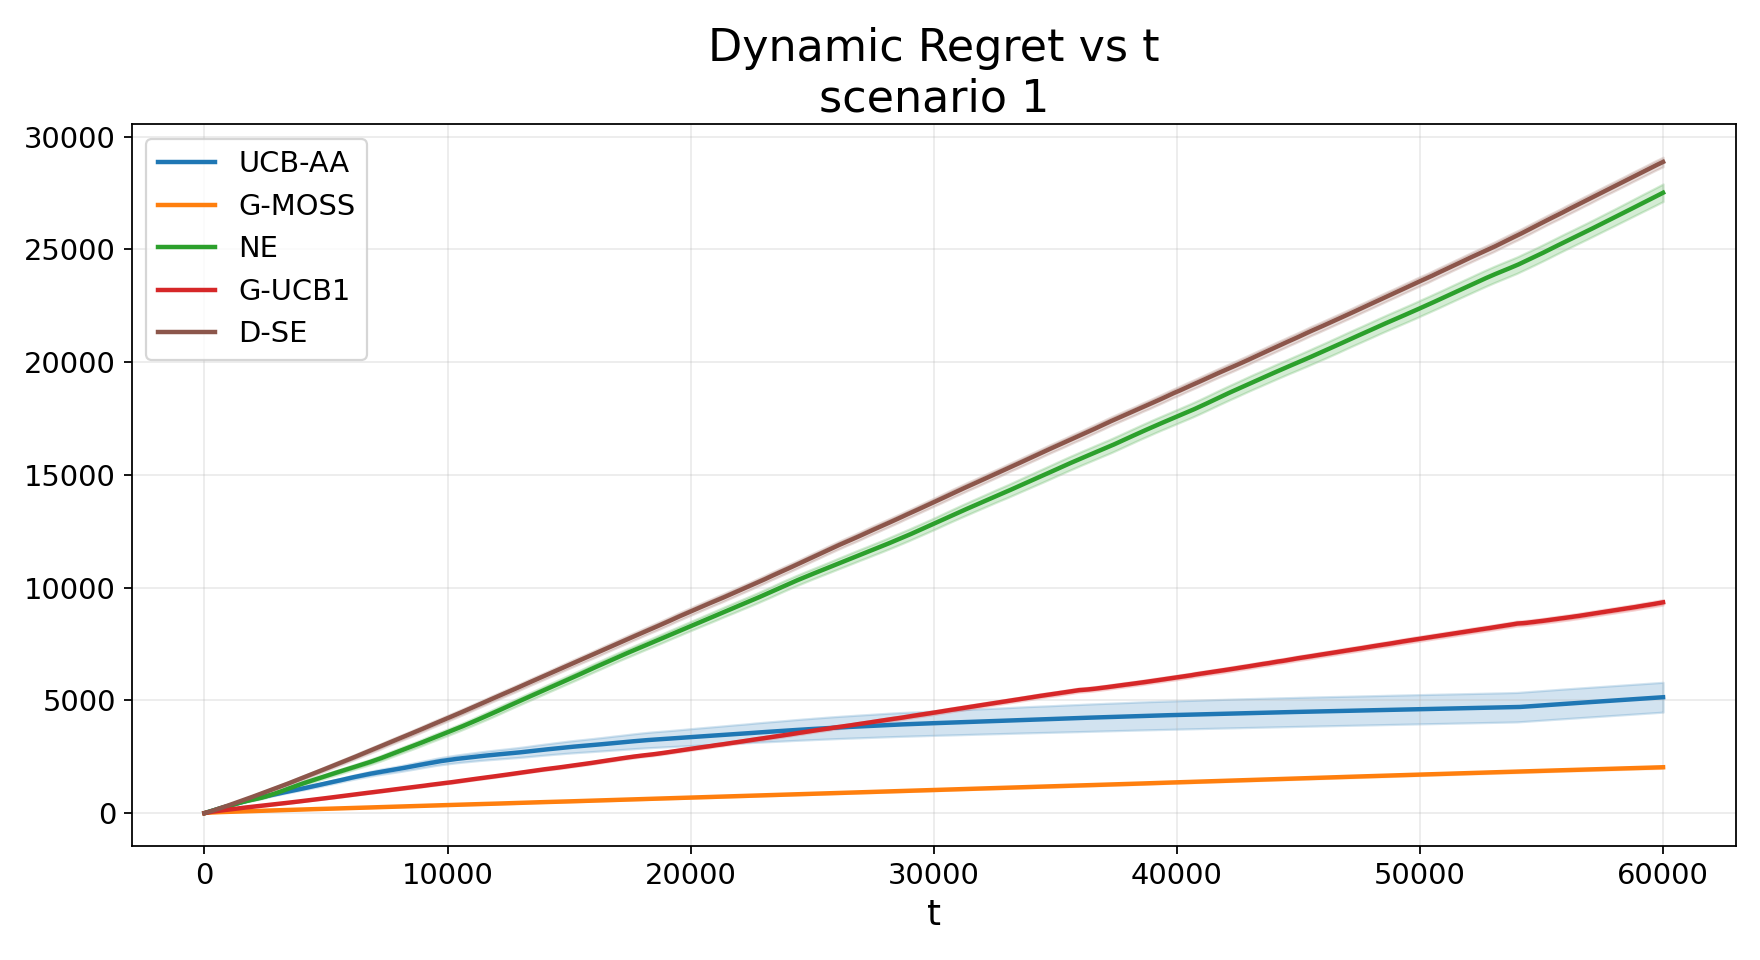
\includegraphics[width=0.9\textwidth]{scenario_C_dynamic_regret_vs_t.png}

    \smallskip
    \textit{(a) Cumulative dynamic regret (Scenario 1)}
    \vspace{8mm}

    \medskip
    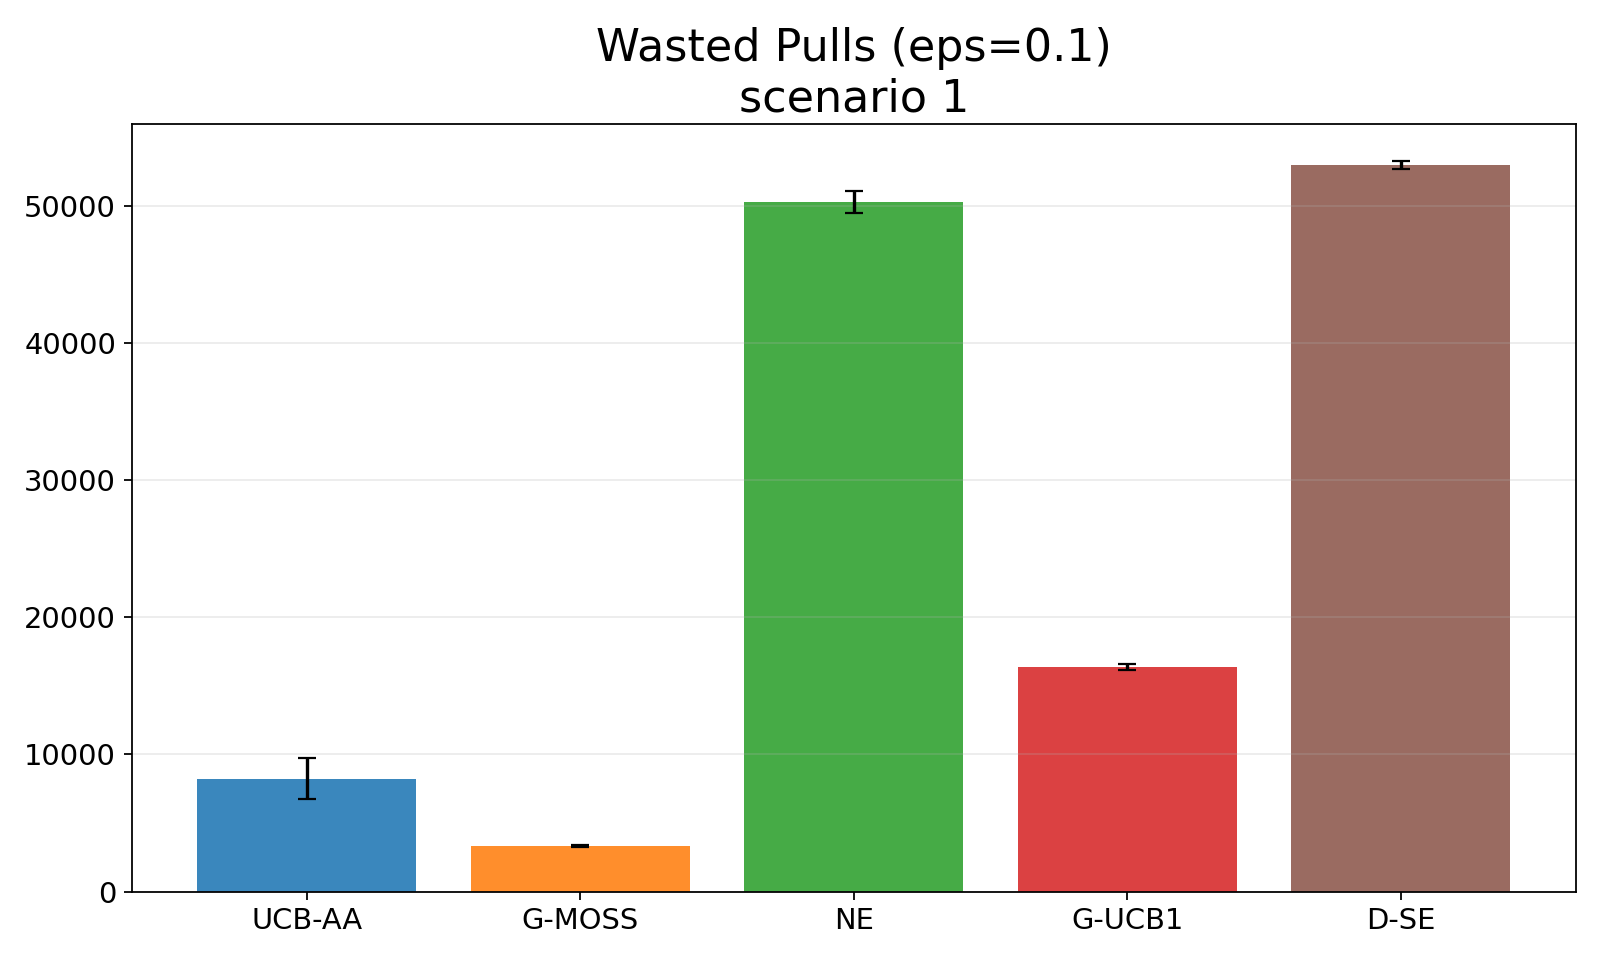
\includegraphics[width=0.9\textwidth]{scenario_C_wasted_pulls_eps_0_1.png}

    \smallskip
    \textit{(b) Wasted pulls (Scenario 1)}
    \caption{Experimental results for Scenario 1 (Progressive step-up arrivals). Panel (a) shows cumulative dynamic regret, and panel (b) compares wasted pulls ($W_T$) and the final number of active arms. Results are averaged over 100 independent runs.}
    \label{fig:scenario_a_results}
\end{figure}

\begin{figure}[htbp]
    \centering
    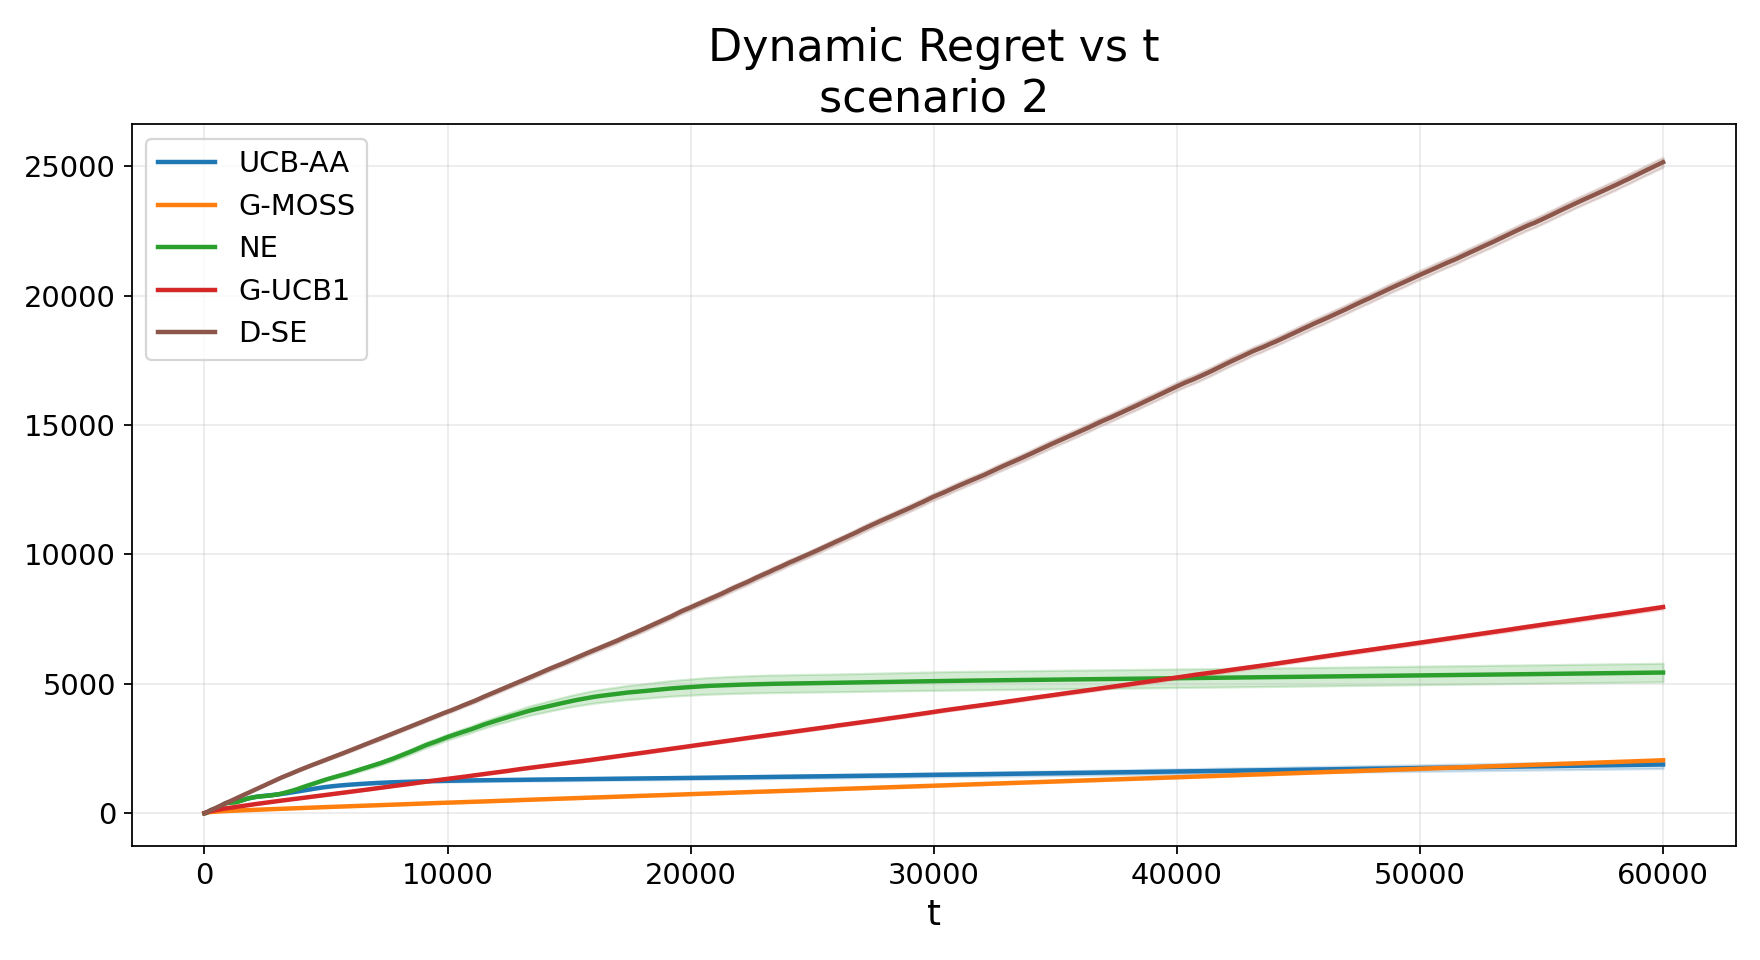
\includegraphics[width=0.9\textwidth]{scenario_E_dynamic_regret_vs_t.png}

    \smallskip
    \textit{(a) Cumulative dynamic regret (Scenario 2)}
    \vspace{8mm}

    \medskip
    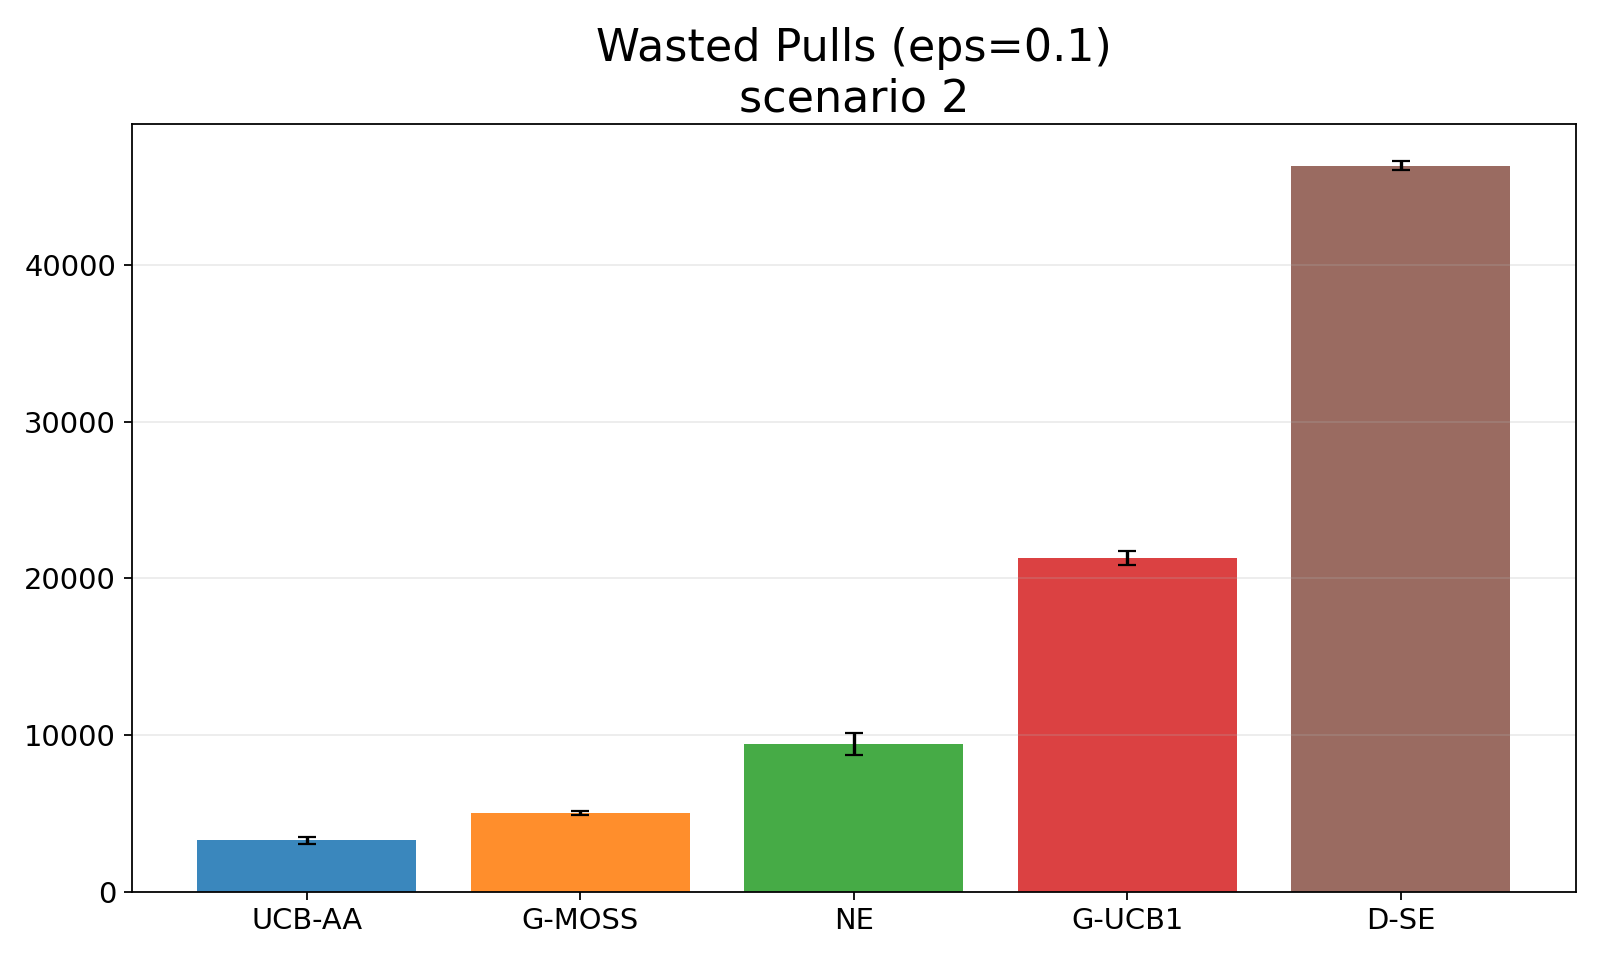
\includegraphics[width=0.9\textwidth]{scenario_E_wasted_pulls_eps_0_1.png}

    \smallskip
    \textit{(b) Wasted pulls (Scenario 2)}
    \caption{Experimental results for Scenario 2 (Near-tied top set). UCB-AA's explicit elimination mechanism maintains a compact decision space while achieving regret performance comparable to Growing MOSS.}

\end{figure}

\begin{figure}[htbp]
    \centering
    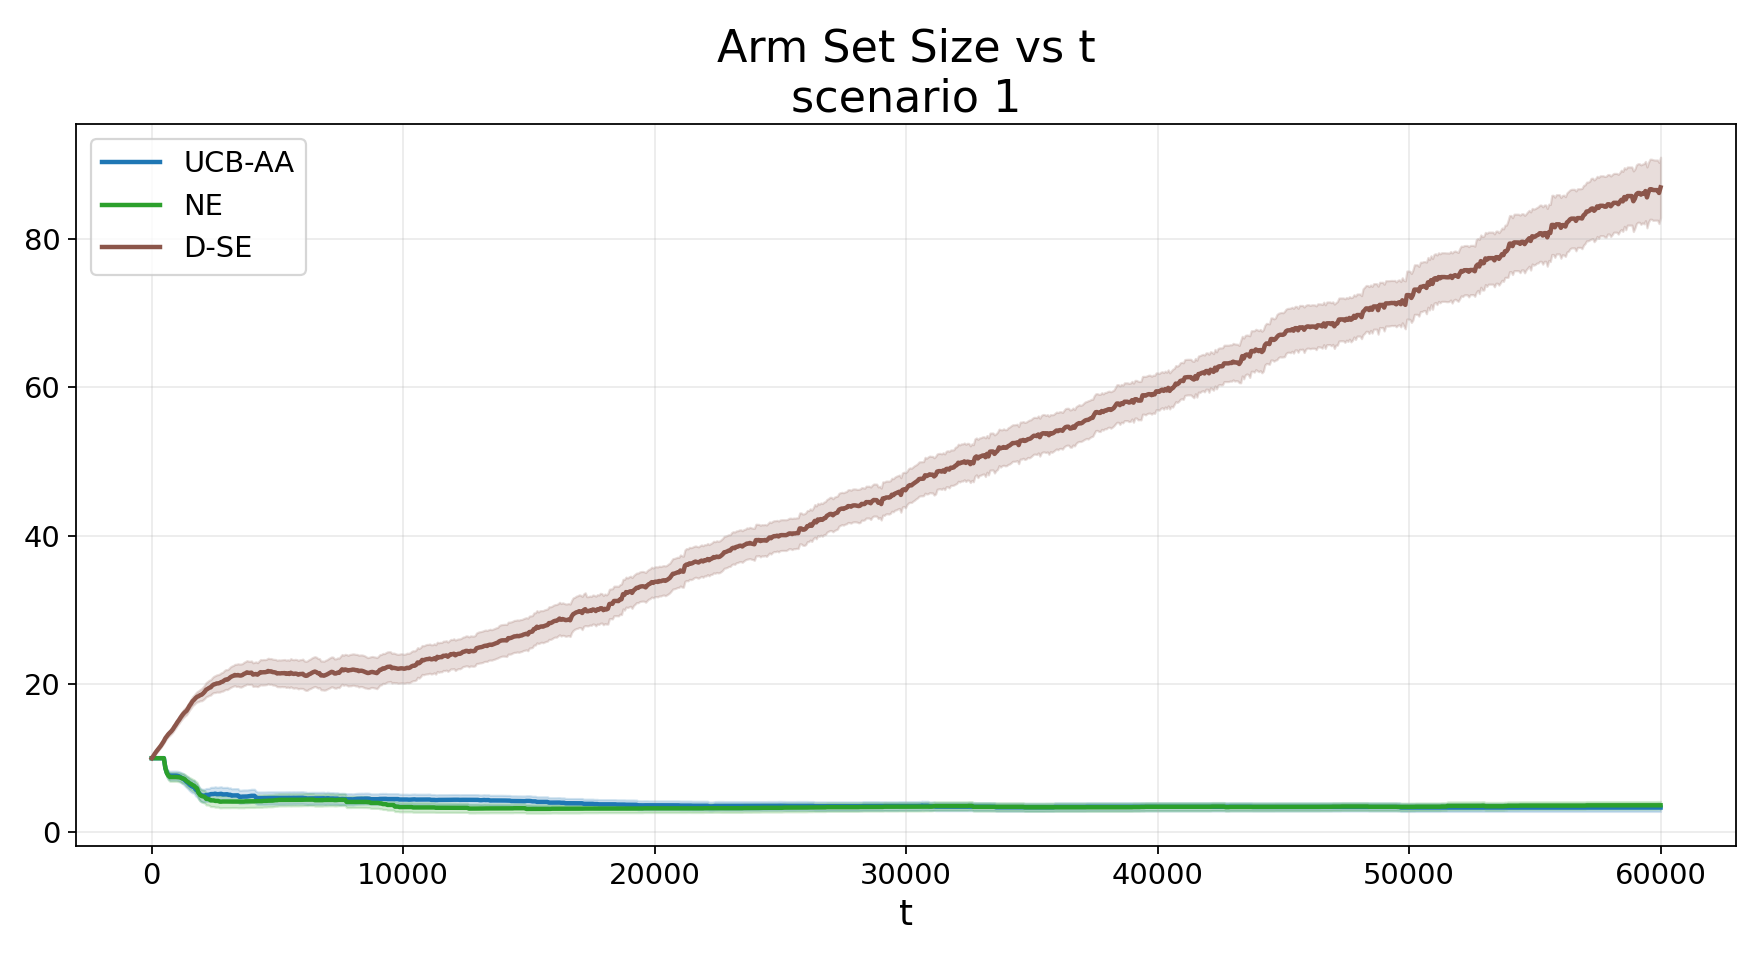
\includegraphics[width=0.9\textwidth]{scenario_C_arm_set_size_vs_t.png}

    \smallskip
    \textit{(a) Active arm size (Scenario 1)}
    \vspace{8mm}

    \medskip
    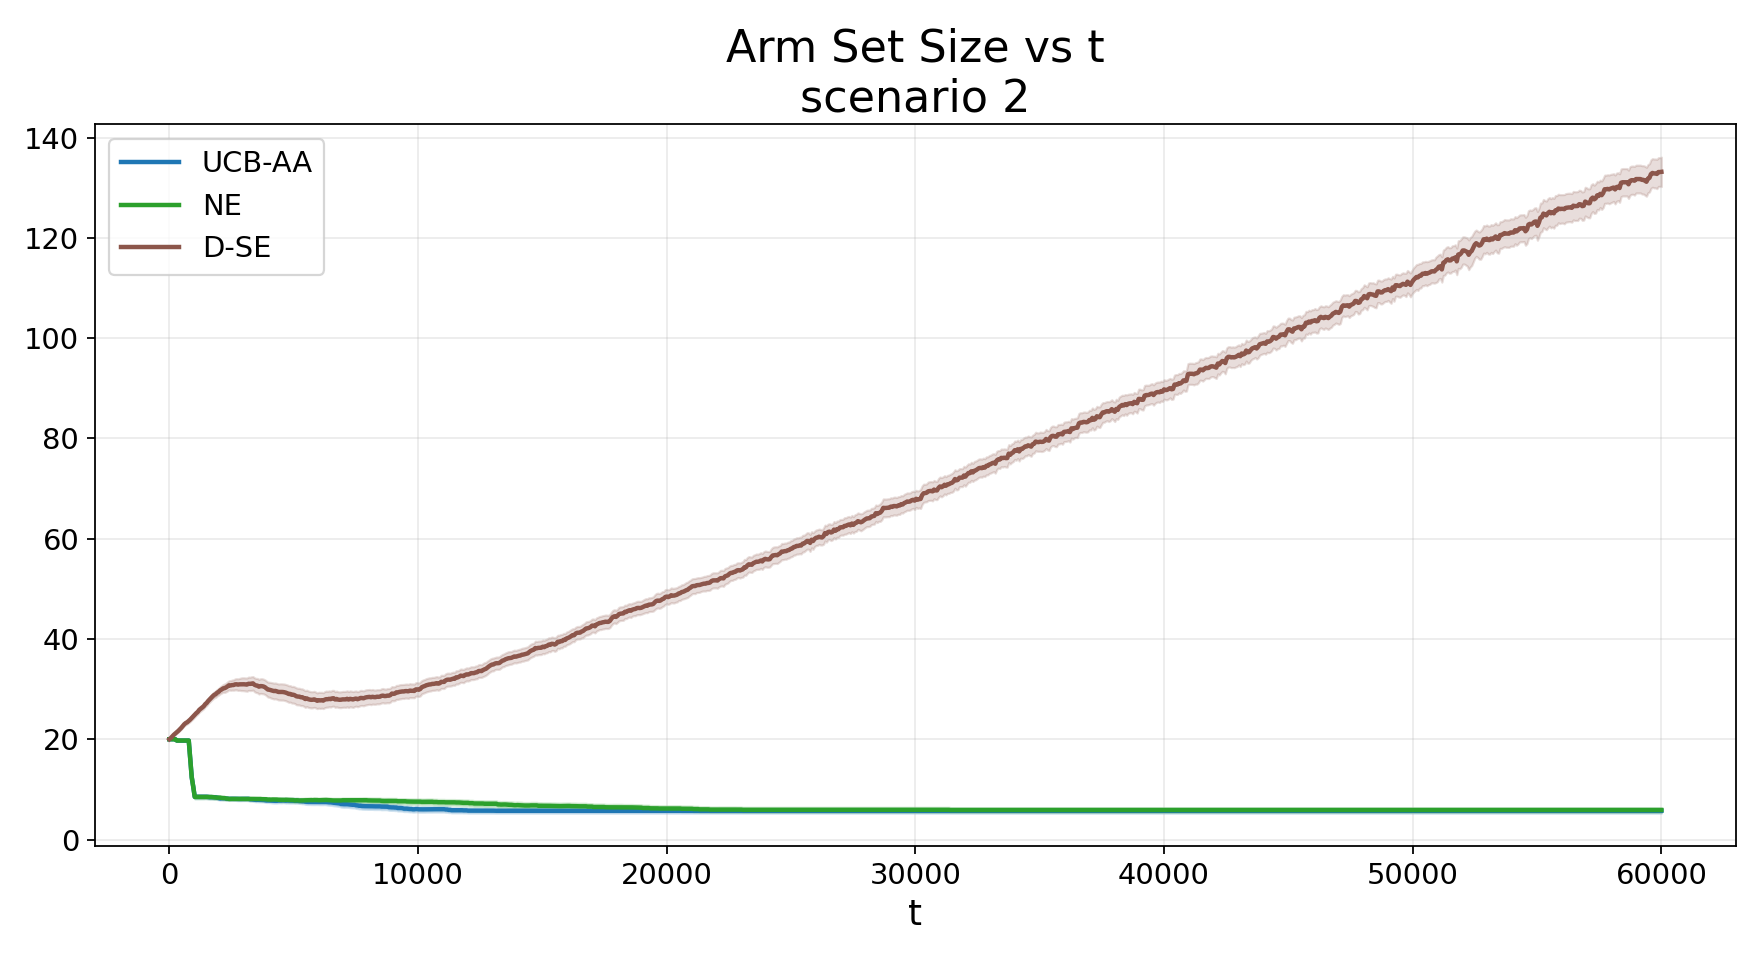
\includegraphics[width=0.9\textwidth]
    {scenario_E_arm_set_size_vs_t.png}

    \smallskip
    \textit{(b) Active arm size (Scenario 2)}
    \caption{Active arm size for two scenarios. UCB-AA's explicit elimination mechanism maintains a compact decision space while achieving regret performance comparable to Growing MOSS.}
\end{figure}

The simulation results show that UCB-AA substantially reduces the number of wasted pulls
($W_T$) relative to Growing UCB1 and the elimination-based baselines. The main reason is that
newly arriving arms are not allowed to compete immediately on equal footing with well-sampled
incumbents. Instead, UCB-AA uses a buffered pre-elimination step to screen out clearly inferior
late arrivals before full competition, thereby protecting the sampling budget of the currently
most competitive arms. By contrast, Growing UCB1 continues to allocate exploration to each new
arrival through its uncertainty bonus, while Naive Elimination and Dynamic SE treat new and old
arms too symmetrically at entry, leading to larger regret.

A second advantage of UCB-AA is that it maintains a compact active set whose members have
survived repeated statistical comparisons over time. Methods such as Growing UCB1 and Growing MOSS do not explicitly prune the arm
set once arms arrive, whereas UCB-AA actively shrinks its working pool $|\mathcal{C}_t|$ through
pre-elimination and formal elimination. As a result, UCB-AA not only controls regret well, but
also returns a smaller set of arms that have survived repeated statistical comparisons and are
therefore more likely to be genuinely competitive.

% At the same time, UCB-AA does not uniformly dominate Growing MOSS in cumulative dynamic regret
% ($R_T$); instead, their regret levels are often comparable. This reflects the cost of explicit
% hard elimination. In UCB-AA, an arm is removed only when its upper confidence bound falls below
% the largest lower confidence bound among the surviving arms,
% \(
% UCB_j < \max_i LCB_i.
% \)
% Because this rule requires strong evidence, UCB-AA may spend somewhat more samples on newly
% arrived borderline arms before discarding them. By contrast, Growing MOSS performs only a soft
% form of elimination: weak arms are downweighted when their indices fall behind, but they remain
% eligible for future sampling if uncertainty later widens. This distinction is important in the
% arriving-arm setting. Although soft elimination can reduce short-run exploration cost, explicit
% certification is often preferable in an expanding action space, because it prevents repeated
% revisits to clearly inferior arrivals and thereby mitigates the AID effect predicted
% by the theory.

At the same time, UCB-AA does not uniformly dominate Growing MOSS in cumulative dynamic regret
($R_T$); instead, their regret levels are often comparable, and Growing MOSS can be slightly
better in settings where many arms are near-tied. This reflects the cost of explicit hard
elimination. In UCB-AA, an arm is removed only when its upper confidence bound falls below
the largest lower confidence bound among the surviving arms,
\(
UCB_j < \max_i LCB_i.
\)
Because this rule requires strong evidence, UCB-AA may spend additional samples to certify that
a borderline arm is truly inferior before discarding it. By contrast, Growing MOSS performs only
a soft form of elimination: weak arms receive fewer pulls when their indices fall behind, but
they remain in the available set and can be sampled again if their uncertainty remains large.

This trade-off also indicates when hard elimination is useful. If the only objective is cumulative
regret over a moderate horizon and keeping all arrived arms active is essentially free, then soft
index-based methods such as Growing MOSS can be highly competitive. However, in many arriving-arm
applications, the active set itself is costly to maintain. Examples include recommendation systems
with continuously added items, adaptive A/B testing with many newly launched designs, biomedical
screening or dose-finding studies with costly or risky candidates, and sequential model or policy
selection where each surviving candidate requires repeated evaluation. In such settings, reducing
the active set is not merely a computational convenience; it is part of the statistical objective.
UCB-AA therefore trades a modest amount of additional exploration for certified pruning of clearly
inferior late arrivals, thereby controlling both wasted pulls and the operational burden created
by an expanding action space.



\section{Discussion}\label{sec:Discussion}


We studied stochastic multi-armed bandits with arriving arms, where the available action
set expands over time and the performance is measured against the best currently available arm. The distinct features of arrival information discrepancy (AID) and drifting benchmark (DB) depart from the classical fixed-oracle benchmark and creates two
coupled statistical challenges: repeated certification of newly arriving competitors and a moving target to catch up.

Our main contribution shows that these challenges can be handled in a structured way. The round-based reduction separates the principal certification burden from the additional delay induced by benchmark movement, while UCB-AA uses a pre-elimination stage to screen late arrivals before they enter full competition. Under suitable control of gap evolution, this yields sublinear regret together with a compact active set. The lower-bound regimes further clarify that the hardness of MAB-AA has multiple sources: the static regime recovers the classical logarithmic identification barrier, distractor arrivals induce cumulative certification costs, and near-tied improvements create a local-testing difficulty under a drifting benchmark.

Several extensions are natural. One direction is to incorporate contextual information or arm-level covariates when  available, which may improve reward via individualization as well as the screening efficiency for newly arriving arms. Another direction is to study settings with post-arrival reward drift, while retaining the central focus on how an expanding action set affects exploration and regret. Finally, the arriving-arm framework can be extended to settings involving delayed feedback, operational resource constraints, and arrival processes calibrated from real application data.

\printbibliography

% % The authors declare no conflicts of interest.

\newpage

\phantomsection\label{supplementary-material}
\bigskip


\clearpage
\appendix
\setcounter{page}{1}
\renewcommand{\thepage}{S-\arabic{page}}

\numberwithin{theorem}{section}
\numberwithin{lemma}{section}
\numberwithin{proposition}{section}
\numberwithin{corollary}{section}
\numberwithin{assumption}{section}
\numberwithin{definition}{section}
\numberwithin{example}{section}
\numberwithin{note}{section}

\begin{center}

{\large\bf Supplementary Material for \\ “Multi-Armed Bandits with Arriving Arms: Sequential Screening, Dynamic Regret, and Sublinear Guarantees”}

\if1\anon
Deqi Zheng\textsuperscript{1,*},
Xiaoyang Xu\textsuperscript{1,*},
and Yuhong Yang\textsuperscript{2,$\dagger$}\\[0.4em]

\textsuperscript{1}Qiuzhen College, Tsinghua University\\
\textsuperscript{2}Yau Mathematical Sciences Center, Tsinghua University\\[0.4em]
{\footnotesize
\textsuperscript{*}The first two authors contributed equally to this work.\\
\textsuperscript{$\dagger$}Corresponding author. Email: \texttt{yyangsc@mail.tsinghua.edu.cn}
}
\fi

\end{center}

This supplementary material is organized as follows.

\begin{itemize}
    \item \textbf{Section A} contains the proofs of the main theoretical results:
    \begin{itemize}
        \item \textbf{Section~\ref{sec: Auxiliary Lemmas}}: Present some auxiliary lemmas and necessary proofs;
        \item \textbf{Section~\ref{sec:Proof of thm:ucb-aa-upper}}: Proof of Theorem~\ref{thm:ucb-aa-upper};
        \item \textbf{Section~\ref{sec:Proof of cor:ucb_aa_simplified}}: Proof of Corollary~\ref{cor:ucb_aa_simplified};
        \item \textbf{Section~\ref{sec:Proof of prop:delay_cum}}: Proof of Proposition~\ref{prop:delay_cum};
        \item \textbf{Section~\ref{sec:Proof of cor:online_gap_independent}}: Analysis of Online UCB-AA and Proof of Corollary~\ref{cor:online_gap_independent};
        \item \textbf{Section~\ref{sec:Proof of thm:static-lb-local-quadratic}}: Proof of 
        Theorem~\ref{thm:static-lb-local-quadratic};
        \item  \textbf{Section~\ref{sec:Proof of thm:distractor-lb-local}}: Proof of Theorem~\ref{thm:distractor-lb-local};
        \item  \textbf{Section~\ref{sec:Proof of thm:prog-lb-general}}: Proof of Theorem~\ref{thm:prog-lb-general}.
    \end{itemize}
    
    \item \textbf{Section B} provides the analysis of four concrete cases:
    \begin{itemize}
        \item \textbf{Section~\ref{sec:Analysis of exp:static}}: Analysis of Example~\ref{exp:static};
        \item \textbf{Section~\ref{sec:Analysis of exp:distractors}}: Analysis of Example~\ref{exp:distractors};
        \item \textbf{Section~\ref{sec:Analysis of exp:monotone-near-tied-ladder}}: Analysis of Example~\ref{exp:monotone-near-tied-ladder};
        \item \textbf{Section~\ref{sec:The Case that Gaps Vary Dramatically}}: Analysis of UCB-AA in the Case that Gaps Vary Dramatically.
    \end{itemize}
    
    \item \textbf{Section C} presents the details of the numerical experiments, including the experimental design, environment parameters, implementation details, and pseudocodes for algorithms.
\end{itemize}

\section{Proofs}
\subsection{Auxiliary Lemmas}\label{sec: Auxiliary Lemmas}
%====================================================
%% Auxiliary Lemmas
%====================================================

We first collect several standard information-theoretic facts used in the lower-bound
arguments. Lemma~\ref{lem:binary-reduction} follows from the data-processing inequality for relative entropy
applied to the binary statistic \(\mathbf{1}_A\)
\parencite[see, e.g.,][]{coverThomas2006,lattimoreSzepesvari2020}.
Lemmas~\ref{lem:bernoulli-kl-lower} and \ref{lem:bernoulli-kl-upper} are elementary bounds for the Bernoulli KL divergence; in particular,
Lemma~\ref{lem:bernoulli-kl-upper} follows from the standard comparison \(D(P\|Q)\le \chi^2(P,Q)\) specialized
to Bernoulli laws \parencite[see, e.g.,][]{tsybakov2009,lattimoreSzepesvari2020}.
Lemma~\ref{lem:pinsker} is Pinsker's inequality \parencite{pinsker1964,tsybakov2009}. Lemma~\ref{lem:kl-chain-rule} is the
standard change-of-measure, or divergence-decomposition, identity for adaptively sampled
bandit observations \parencite[see, e.g., Lemma~1 of][]{KaufmannCappeGarivier2016};
see also \textcite[Chapter~15]{lattimoreSzepesvari2020}.

\begin{lemma}[Binary reduction for KL]
\label{lem:binary-reduction}
Let $P$ and $Q$ be two probability measures on the same measurable space, and
let $A$ be any measurable event. Then
\[
\mathrm{KL}(P,Q)\ge \mathrm{kl}(P(A),Q(A)),
\]
where
\[
\mathrm{kl}(p,q):=p\log\frac pq+(1-p)\log\frac{1-p}{1-q}
\]
denotes the Bernoulli Kullback--Leibler divergence.
\end{lemma}

\begin{proof}
Apply the data-processing inequality to the measurable map
$x\mapsto \mathbf 1_A(x)$, which sends the original experiment to a Bernoulli
experiment with success probabilities $P(A)$ and $Q(A)$.
\end{proof}

\begin{lemma}[A crude lower bound on Bernoulli KL]
\label{lem:bernoulli-kl-lower}
For any $p\in[0,1]$ and $q\in(0,1)$,
\[
\mathrm{kl}(p,q)\ge p\log\frac1q-\log 2.
\]
\end{lemma}

\begin{proof}
By definition,
\[
\mathrm{kl}(p,q)
=
p\log\frac1q+(1-p)\log\frac1{1-q}+p\log p+(1-p)\log(1-p).
\]
The second term on the right-hand side is nonnegative, while
\[
p\log p+(1-p)\log(1-p)\ge -\log 2.
\]
Combining the two bounds gives the claim.
\end{proof}

\begin{lemma}[Bernoulli KL upper bound]
\label{lem:bernoulli-kl-upper}
For any $p\in[0,1]$ and $q\in(0,1)$,
\[
\mathrm{kl}(p,q)\le \frac{(p-q)^2}{q(1-q)}.
\]
Consequently, if $p\in[0,1]$ and $q\in[\gamma,1-\gamma]$ for some
$\gamma\in(0,1/2]$, then
\[
\mathrm{kl}(p,q)\le \frac{1}{\gamma(1-\gamma)}(p-q)^2.
\]
\end{lemma}

\begin{proof}
For $p\in(0,1)$, the first inequality is standard. The boundary cases
$p=0$ and $p=1$ follow by continuity. The second inequality is immediate from
$q(1-q)\ge \gamma(1-\gamma)$.
\end{proof}

\begin{lemma}[Pinsker's inequality]
\label{lem:pinsker}
For any probability measures $P$ and $Q$,
\[
\mathrm{TV}(P,Q)\le \sqrt{\frac12 \mathrm{KL}(P,Q)}.
\]
\end{lemma}

\begin{lemma}[KL chain rule for adaptive sampling]
\label{lem:kl-chain-rule}
Let $\nu$ and $\nu'$ be two bandit instances, and let $\mathbb P_\nu$ and
$\mathbb P_{\nu'}$ denote the induced laws of the full history
\[
H_T := (I_1,X_1,\dots,I_T,X_T).
\]
Suppose that $\nu$ and $\nu'$ differ only in the reward law of arm $j$, whose
distributions are $P$ and $Q$ on $[0,1]$, respectively. Then
\[
\mathrm{KL}(\mathbb P_\nu,\mathbb P_{\nu'})
=
\mathbb E_\nu[N_j(T)]\,D(P\|Q),
\]
where
\[
N_j(T):=\sum_{t=1}^T \mathbf 1\{I_t=j\}.
\]
In particular, if $P=\mathrm{Bernoulli}(p)$ and
$Q=\mathrm{Bernoulli}(q)$, then
\[
\mathrm{KL}(\mathbb P_\nu,\mathbb P_{\nu'})
=
\mathbb E_\nu[N_j(T)]\,\mathrm{kl}(p,q).
\]
\end{lemma}
\begin{proof}
Let $K_t(\cdot\mid h_{t-1})$ denote the (possibly randomized) action kernel
used by the policy at time $t$, given past history $H_{t-1}=h_{t-1}$.
Since the policy is the same under $\nu$ and $\nu'$, the kernel $K_t$
is identical under the two instances. By the chain rule for KL divergence,
\[
\mathrm{KL}(\mathbb P_\nu,\mathbb P_{\nu'})
=
\sum_{t=1}^T
\mathbb E_\nu\!\left[
\mathrm{KL}\!\left(
\mathcal L((I_t,X_t)\mid H_{t-1})_\nu,\,
\mathcal L((I_t,X_t)\mid H_{t-1})_{\nu'}
\right)\right].
\]
Conditional on $H_{t-1}=h_{t-1}$, the joint law of $(I_t,X_t)$ under $\nu$
is given by
\[
K_t(di\mid h_{t-1})\,M_i(dx),
\]
where $M_i$ is the reward law of arm $i$ under $\nu$; under $\nu'$ the same
expression holds with $M_i'$ in place of $M_i$.
Since the two instances differ only on arm $j$, we have $M_i=M_i'$ for
$i\neq j$, while $M_j=P$ and $M_j'=Q$.
Therefore the conditional KL divergence equals
\[
\mathbf 1\{I_t=j\}\,D(P\|Q),
\]
and hence
\[
\mathrm{KL}(\mathbb P_\nu,\mathbb P_{\nu'})
=
\sum_{t=1}^T
\mathbb E_\nu\!\left[\mathbf 1\{I_t=j\}\,D(P\|Q)\right]
=
\mathbb E_\nu[N_j(T)]\,D(P\|Q).
\]
The Bernoulli specialization is immediate.
\end{proof}


\subsection{Proof of Theorem~\ref{thm:ucb-aa-upper}}
\label{sec:Proof of thm:ucb-aa-upper}
\begin{proof}[Proof of Theorem~\ref{thm:ucb-aa-upper}]
 We analyze the regret $\mathbb{E}(R^{(i)}(\pi)) $ which is generated by each suboptimal arm $i\in A'(\lambda)$ by dividing the entire space into three cases. Define the event 
\begin{align*}
    \tilde{E}_i&=\{ i\in A'(\lambda) \text{ has not been eliminated in or before $\overline{m}_i$-th elimination phase of round $m_i$ }  \}, \\
    \tilde{F}_i&=\{ *(m_i) \in B_{m_i}^{\overline{m}_i} \}.
\end{align*}

Here, if $\overline{m}_i\geq m_i-1$, then $\overline{m}_i$-th elimination phase is the formal elimination phase of round $m_i$; if $\overline{m}_i< m_i-1$, then $\overline{m}_i$-th elimination phase is in the pre-elimination phase. $*(m_i)\in B_{m_i}^{\overline{m}_i}$ means the optimal arm at round $m_i$ remains at the beginning of $\overline{m}_i$-th elimination phase.

Then, we divide the regret into three parts, 
\[\mathbb{E}(R^{(i)}(\pi)) = \underbrace{\mathbb{E}\left(R^{(i)}(\pi)\cdot I_{\tilde{E}_i\cap \tilde{F}_i}\right)}_{\text{case (a)}} + \underbrace{\mathbb{E}\left(R^{(i)}(\pi)\cdot I_{\tilde{E}_i^c}\right)}_{\text{case (b1)}} + \underbrace{\mathbb{E}\left(R^{(i)}(\pi)\cdot I_{\tilde{E}_i\cap\tilde{F}_i^c}\right)}_{\text{case (b2)}}.\]
Now, we calculate the upper bounds for the regret of these three parts, respectively.

\textbf{Case (a):} \textit{ If suboptimal arm $i\in A'(\lambda)$ was not eliminated in or before the $\overline{m}_i$-th elimination phase of round $m_i$, and $*(m_i)\in B_{m_i}^{\overline{m}_i}$. }

If $i\in G_1(\lambda)\cup G_2(\lambda)$, then $\overline{m}_i=\tilde{m}_i$. We have  \( \sqrt{\frac{\log(N \tilde{\Delta}_{\tilde{m}_i}^2)}{2n_{\tilde{m}_i}}} \leq \frac{1}{2}\tilde{\Delta}_{\tilde{m}_i} < \frac{1}{4}\Delta_i(m_i) \) by the definition of $\tilde{m}_i$, if \begin{align}
    \hat{r}_i(n_p) \leq r_i + \sqrt{\frac{\log(N \tilde{\Delta}_{p}^2)}{2n_{p}}} \label{suboptimal is bad A-3}
\end{align}
and  
\begin{align}
    \hat{r}_{*(m)}(n_p) \geq r_{*(m)} - \sqrt{\frac{\log(N \tilde{\Delta}_{p}^2)}{2n_{p}}} \label{optimal is good A-3}
\end{align}
hold for $m = m_i,\; p=\tilde{m}_i$, then we have:  
\begin{align*}
    \hat{r}_i(n_{\tilde{m}_i}) + \sqrt{\frac{\log(N \tilde{\Delta}_{\tilde{m}_i}^2)}{2n_{\tilde{m}_i}}} &\leq r_i + 2\sqrt{\frac{\log(N \tilde{\Delta}_{\tilde{m}_i}^2)}{2n_{\tilde{m}_i}}} < r_i + \Delta_i(m_i) - 2\sqrt{\frac{\log(N \tilde{\Delta}_{\tilde{m}_i}^2)}{2n_{\tilde{m}_i}}} \\
    &= r_{*(m_i)} - 2\sqrt{\frac{\log(N \tilde{\Delta}_{\tilde{m}_i}^2)}{2n_{\tilde{m}_i}}} \leq \hat{r}_{*(m_i)}(n_{\tilde{m}_i}) - \sqrt{\frac{\log(N \tilde{\Delta}_{\tilde{m}_i}^2)}{2n_{\tilde{m}_i}}}.
\end{align*}
Further, by the assumption that arm $i$ and $*(m_i)$ coexist and the elimination rule, \( i \) will be eliminated, and $i$ is pulled no more than $n_{\tilde{m}_i}$ times. Besides, using the Chernoff-Hoeffding bound, we have for $p=0,1,\cdots$ and $m=0,1\cdots$:
\begin{align}
    \mathbb{P}\left( \hat{r}_i(n_p) > r_i + \sqrt{\frac{\log(N \tilde{\Delta}_{p}^2)}{2n_{p}}} \right)    \leq \frac{1}{N \tilde{\Delta}_{p}^2}
    \label{suboptimal is good A-3}
\end{align}
\begin{align}
    \mathbb{P}\left( \hat{r}_{*(m)}(n_p) < r_{*(m)} - \sqrt{\frac{\log(N \tilde{\Delta}_{p}^2)}{2n_{p}}} \right) \leq \frac{1}{N \tilde{\Delta}_{p}^2} 
    \label{optimal is bad A-3}
\end{align}
Take $p=\tilde{m}_i,\; m=m_i$, so the upper bound of the probability that arm \( i \) is not eliminated in or before the $\overline{m}_i$-th elimination phase of round $m_i$ is $\frac{2}{N \tilde{\Delta}_{\tilde{m}_i}^2}$.

If $i\in G_3(\lambda)$, then $\overline{m}_i=m_i-1$ and $m_i>t_i$, which means that the optimal arm $*(m_i)$ arrives at the beginning of round $m_i$, i.e. $t_{*(m_i)}=m_i$, while arm $i$ is already present before round $m_i$. Note that $\Delta_i(m_i)=r_{*(m_i)}-r_i$. According to the workflow of UCB-AA, the suboptimal arm $i$ is therefore expected to be eliminated during the $\overline{m}_i$-th elimination phase of round $m_i$. By the definition of $\tilde{m}_i$, if
\begin{align}
    \hat{r}_i(n_{m_i-1}) \leq r_i - \sqrt{\frac{\log(N \tilde{\Delta}_{m_i-1}^2)}{2n_{m_i-1}}}+\tilde{\Delta}_{\tilde{m}_i} \label{eq: suboptimal is bad A-3 G-3}
\end{align}
and  
\begin{align}
    \hat{r}_{*(m_i)}(n_{m_i-1}) \geq r_{*(m_i)} + \sqrt{\frac{\log(N \tilde{\Delta}_{m_i-1}^2)}{2n_{m_i-1}}} -\tilde{\Delta}_{\tilde{m}_i}
    \label{eq: optimal is good A-3 G-3}
\end{align}
hold, then we have:  
\begin{align*}
    \hat{r}_i(n_{m_i-1}) + \sqrt{\frac{\log(N \tilde{\Delta}_{m_i-1}^2)}{2n_{m_i-1}}} &\leq r_i + \tilde{\Delta}_{\tilde{m}_i}\\
   \left(\tilde{\Delta}_{\tilde{m}_i}<\frac{1}{2}\Delta_i(m_i)\right) &< r_{*(m_i)} -\tilde{\Delta}_{\tilde{m}_i} \leq \hat{r}_{*(m_i)}(n_{m_i-1}) - \sqrt{\frac{\log(N \tilde{\Delta}_{m_i-1}^2)}{2n_{m_i-1}}}.
\end{align*}
By the elimination rule, \( i \) will be eliminated by the optimal arm $*(m_i)$. Again, using the Chernoff-Hoeffding bound, we have:
\begin{align}
   & \mathbb{P}\left( \hat{r}_i(n_{m_i-1})>r_i - \sqrt{\frac{\log(N \tilde{\Delta}_{m_i-1}^2)}{2n_{m_i-1}}}+\tilde{\Delta}_{\tilde{m}_i} \right) \notag\\   
   \leq &\exp\left(-2n_{m_i-1}\left(\tilde{\Delta}_{\tilde{m}_i} - \sqrt{\frac{\log(N \tilde{\Delta}_{m_i-1}^2)}{2n_{m_i-1}}}\right)^2\right)\leq \frac{1}{N\tilde{\Delta}_{\tilde{m}_i}^2}.
    \label{eq: suboptimal is good A-3 G-3}
\end{align}
The last inequality of \eqref{eq: suboptimal is good A-3 G-3} comes from the fact that $n_{\tilde{m}_i}\leq n_{m_i-1}$ and
\[\sqrt{\frac{\log(N \tilde{\Delta}_{m_i-1}^2)}{2n_{m_i-1}}}\leq \frac{1}{2}\tilde{\Delta}_{m_i-1}\leq \frac{1}{2}\tilde{\Delta}_{\tilde{m}_i},\quad \sqrt{\frac{\log(N \tilde{\Delta}_{\tilde{m}_i}^2)}{2n_{\tilde{m}_i}}}\leq \frac{1}{2}\tilde{\Delta}_{\tilde{m}_i}.\]

Similarly, we can conclude that
\begin{align}
    \mathbb{P}\left( \hat{r}_i(n_{m_i-1})>r_i - \sqrt{\frac{\log(N \tilde{\Delta}_{m_i-1}^2)}{2n_{m_i-1}}}+\tilde{\Delta}_{\tilde{m}_i} \right) 
   \leq \frac{1}{N\tilde{\Delta}_{\tilde{m}_i}^2}.
    \label{eq: optimal is bad A-3 G-3}
\end{align}

Thus, the regret contributed by arm $i$, conditioned on case (a), is upper bounded by
\[
R_i \coloneqq n_{t_i}\Delta_i(t_i) + \sum_{m = t_i + 1}^{M} (n_m - n_{m-1})\Delta_i(m),
\]
and the corresponding total expected regret contributed by each suboptimal arm $i\in A'(\lambda)$ in case (a) is upper-bounded by:
\[\sum_{i\in A'(\lambda)}\frac{2}{N \tilde{\Delta}_{\tilde{m}_i}^2}\cdot\left[n_{t_i}\Delta_i(t_i) + \sum_{m = t_i + 1}^{M} (n_m - n_{m-1})\Delta_i(m)\right]=\sum_{i\in A'(\lambda)}\frac{2R_i}{N\tilde{\Delta}_{\tilde{m}_i}^2}.\]

\textbf{Case (b):} \textit{For a suboptimal arm \( i \in A'(\lambda)\), either it is eliminated in or before the $\overline{m}_i$-th elimination phase of round $m_i$, or \( *(m_i) \notin B_{m_i}^{\overline{m}_i} \) (i.e., the optimal arm of round \( m_i \) is eliminated in the $\overline{m}_i$-th elimination phase of round $m_i$ or earlier).  }

We divide it into two smaller cases:

\textbf{Case (b1):}\textit{ $i$ is eliminated in or before the $\overline{m}_i$-th elimination phase of round $m_i$.  }

If $i\in G_1(\lambda)$, then $m_i=t_i$, and $\overline{m}_i=\tilde{m}_i$. In this case, arm $i$ is eliminated in the $\tilde{m}_i$-th elimination phase of round $m_i$. Therefore, the random regret contributed by arm $i$ is upper bounded by
\[\tilde{S}_i\coloneqq n_{\tilde{m}_i}\cdot \Delta_i(t_i),\quad i\in G_1(\lambda).\]

If $i\in G_2(\lambda)$, then $m_i>t_i$ and $\overline{m}_i=\tilde{m}_i$, and the total number of times arm \( i \) can be pulled does not exceed $n_{\tilde{m}_i}$. Hence, the random regret of arm $i$ is upper bounded by
\[\tilde{S}_i\coloneqq n_{t_i}\Delta_i(t_i) + \sum_{m = t_i + 1}^{\overline{m}_i} (n_m - n_{m-1})\Delta_i(m), \quad i\in G_2(\lambda).\]

If $i\in G_3(\lambda)$, then $m_i>t_i$ and $\overline{m}_i=m_i-1$, arm $i$ is eliminated in or before the $\overline{m}_i$-th elimination phase of round $m_i$. By the definition of the algorithm, arm $i$ has already been pulled $n_{m_i-1}$ times in total. Thus, the corresponding upper bound on the random regret of arm $i$ is
\[\tilde{S}_i\coloneqq n_{t_i}\Delta_i(t_i)+\sum_{m=t_i+1}^{\overline{m}_i}(n_m-n_{m-1})\Delta_i(m),\quad i\in G_3(\lambda).\]

Therefore, the corresponding total expected regret in case (b1) is upper bounded by 
\[\sum_{i \in A'(\lambda)} \tilde{S}_i.\]

\textbf{Case (b2):}\textit{ If suboptimal arm \( i \in A'(\lambda) \) was not eliminated in or before the $\overline{m}_{i}$-th elimination phase of round $m_i$, and \( *(m_i) \notin B_{m_i}^{\overline{m}_i} \). }  

If $i\in G_2(\lambda)$, then $\overline{m}_i=\tilde{m}_i=m_i$. Under the assumption of case (b2), $*(m_i)$ must have been eliminated in round \( t_{*(m_i)} \leq m_* \leq m_i \) by some suboptimal arm \( j \). Note that if \eqref{suboptimal is bad A-3} and \eqref{optimal is good A-3} hold at \(p= m_{**} \) for $j$ and $m=m_i$ respectively, then \( *(m_i) \) will not be eliminated by \( j \) in the $m_{**}$-th elimination phase of round $m_*$, here $t_{*(m_i)}\leq m_*\leq m_i$. Therefore, the upper bound of the probability that \( *(m_i) \) is eliminated by \( j \) in the $m_{**}$-th elimination phase of round $m_*$ is \( \frac{2}{N \tilde{\Delta}_{m_{**}}^2} \). We have \( \Delta_j(M) > \Delta_{*(m_i)}(M) \geq 0 \) and \( t_j \leq m_* \leq m_i \). 

On the other hand, we observe from the definitions that all possible elimination phases in which the optimal arm $*(m_i)$ is eliminated in round $ t_{*(m_i)} \leq m_* \leq m_i $ are as follows:
\begin{align*}
    J_{m_*}:&=\{m_{**}:\text{$*(m_i)$ can be eliminated in the } m_{**} \text{-th elimination phase of round $m_*$}\}\\
    &=\begin{cases}
    \{0,1,\cdots, m_*\},& m_*=t_{*(m_i)};\\
    \{m_*-1,\, m_*\}, &t_{*(m_i)}<m_*\leq m_i.
\end{cases}
\end{align*}

Thus, we have: 
\begin{align}
&\;\mathbb{P}\left(\tilde{E}_i\cap\tilde{F}_i^c\right)\notag\\
    \leq &\;\mathbb{P}\left(*(m_i) \text{ is eliminated by some suboptimal arm } j \text{ in some round } m_*,\; t_{*(m_i)} \leq m_* \leq m_i\right)\notag\\
   = &\sum_{m_* = t_{*(m_i)}}^{m_i} \mathbb{P}\left(*(m_i) \text{ is eliminated by some suboptimal arm } j \text{ in round } m_*\right) \notag\\
\leq & \sum_{m_* = t_{*(m_i)}}^{m_i} \sum_{\substack{j :\,t_j\leq m_*\\j\neq *(m_i)}}\sum_{m_{**}\in J_{m_*}} \!\!\mathbb{P}\left(*(m_i) \text{ is eliminated by } j \text{ in $m_{**}$-th elimination phase of round } m_*\right) \notag\\
\leq & \sum_{m_* = t_{*(m_i)}}^{m_i}  \sum_{\substack{j :\,t_j\leq m_*\\j\neq *(m_i)}} \sum_{m_{**}=0}^{m_*}\frac{2}{N \tilde{\Delta}_{m_{**}}^2}\leq \sum_{m_* = t_{*(m_i)}}^{m_i}  \sum_{\substack{j :\,t_j\leq m_*\\j\neq *(m_i)}} \frac{3}{N \tilde{\Delta}_{m_*}^2}\leq\sum_{m_* = t_{*(m_i)}}^{m_i}   \frac{3\left(K(m_i)-1\right)}{N \tilde{\Delta}_{m_*}^2}\notag\\
<& \;\frac{3\left(K(m_i)-1\right)}{N } \sum_{m_* = 0}^{m_i}   \frac{1}{ \tilde{\Delta}_{m_*}^2} < \;\frac{3\left(K(m_i)-1\right)}{N}\cdot \frac{4}{3}\cdot4^{m_i}=\frac{4\left(K(m_i)-1\right)}{N\tilde{\Delta}_{m_i}^2}\notag\\
=&\frac{4\left(K(m_i)-1\right)}{N\tilde{\Delta}_{\tilde{m}_i}^2}, \quad i\in G_2(\lambda).
\label{eq: UCB-A3 G-2 b2}
\end{align}

If $i\in G_1(\lambda)$, then $t_i=m_i$ and $\overline{m}_i=\tilde{m}_i$. In this case, we further distinguish whether the optimal arm $*(m_i)$ arrives simultaneously with arm $i$; that is, whether $t_{*(m_i)}=t_i=m_i$.
\begin{itemize}
    \item If $t_{*(m_i)}=t_i=m_i$, then we have
    \begin{align*}
        &\mathbb{P}\left(\tilde{E}_i\cap\tilde{F}_i^c\right)\\
        \!\!\!\!\!\!\!\!\!\leq \;&\mathbb{P}\left(*(m_i) \text{ is eliminated by some arm } j \text{ in or before $\tilde{m}_i$-th elimination phase in round } m_i\right) \\
        \leq \;& \sum_{\substack{j :\,t_j\leq m_i\\j\neq *(m_i)}}\sum_{m_{*}=0}^{\tilde{m}_i}\frac{2}{N \tilde{\Delta}_{m_{*}}^2}<\frac{4\left(K(m_i)-1\right)}{N\tilde{\Delta}_{\tilde{m}_i}^2}.
    \end{align*}
    \item If $t_{*(m_i)}<t_i=m_i$, by the definition of the UCB-AA algorithm, we know the optimal arm $*(m_i)$ must have been eliminated before the beginning of round $m_i$. We make the following partition:
\begin{align}
\mathbb{P}\left(\tilde{E}_i\cap\tilde{F}_i^c\right)=&\mathbb{P}\left(\tilde{E}_i\cap\tilde{F}_i^c\cap\{\text{$*(m_i)$ is eliminated in or before round }\tilde{m}_i\}\right)\notag\\
+&\mathbb{P}\left(\tilde{E}_i\cap\tilde{F}_i^c\cap\{\text{$*(m_i)$ is eliminated after round }\tilde{m}_i\}\right).
\label{eq: partition UCB-A3 G-1 b2}
\end{align}
We analyze these two items separately. Without loss of generality, we assume $t_{*(m_i)}\leq \tilde{m}_i$; otherwise, the first term in \eqref{eq: partition UCB-A3 G-1 b2} vanishes. Similar to the method used in \eqref{eq: UCB-A3 G-2 b2}, we obtain an upper bound of the first term:
\begin{align}
    &\mathbb{P}\left(\tilde{E}_i\cap\tilde{F}_i^c\cap\{\text{$*(m_i)$ is eliminated in or before round }\tilde{m}_i\}\right)\notag\\
\leq &\sum _{m_*=t_{*(m_i)}}^{\tilde{m}_i} \mathbb{P}\left(*(m_i) \text{ is eliminated by some suboptimal arm } j \text{ in round } m_*\right)\notag \\
\leq & \sum_{m_* = t_{*(m_i)}}^{\tilde{m}_i} \sum_{\substack{j :\,t_j\leq m_*\\j\neq *(m_i)}}\sum_{m_{**}\in J_{m_*}} \frac{2}{N \tilde{\Delta}_{m_{**}}^2}<\frac{4\left(K(m_i)-1\right)}{N\tilde{\Delta}_{\tilde{m}_i}^2}.
\label{eq: UCB-A3 G-1 b2 first term}
\end{align}
For the second term, we find that if $*(m_i)$ is eliminated after round $\tilde{m}_i$, then by the definition of the UCB-AA algorithm, the empirical average reward obtained from pulling $*(m_i)$ for $n_{\tilde{m}_i}$ times has already been recorded. Thus, we have:
\begin{align}
    &\;\mathbb{P}\left(\tilde{E}_i\cap\tilde{F}_i^c\cap\{\text{$*(m_i)$ is eliminated after round }\tilde{m}_i\}\right)\notag\\
\leq &\;\mathbb{P}\left(\hat{r}_i(n_{\tilde{m}_i}) + \sqrt{\frac{\log(N \tilde{\Delta}_{\tilde{m}_i}^2)}{2n_{\tilde{m}_i}}} >\hat{r}_{*(m_i)}(n_{\tilde{m}_i}) - \sqrt{\frac{\log(N \tilde{\Delta}_{\tilde{m}_i}^2)}{2n_{\tilde{m}_i}}}\right)\leq \frac{2}{N\tilde{\Delta}_{\tilde{m}_i}^2}.
\label{eq: UCB-A3 G-1 b2 second term}
\end{align}
Substituting \eqref{eq: UCB-A3 G-1 b2 first term} and \eqref{eq: UCB-A3 G-1 b2 second term} into \eqref{eq: partition UCB-A3 G-1 b2}, we can get:
\begin{align}
    \mathbb{P}\left(\tilde{E}_i\cap\tilde{F}_i^c\right)\leq \frac{4K(m_i)-2}{N\tilde{\Delta}_{\tilde{m}_i}^2},\quad i\in G_1(\lambda).
    \label{eq: UCB-A3 G-1 b2}
\end{align}
\end{itemize}

If $i\in G_3(\lambda)$, then $t_i<m_i=t_{*(m_i)},\; \tilde{m}_i<m_i$, and $\overline{m}_i=m_i-1$. Thus, by the definition of the UCB-AA algorithm and $\tilde{F}_i^c$, $*(m_i)$ have been eliminated before the beginning of the $(m_i-1)$-th elimination phase of round $m_i$. By $\tilde{m}_i<m_i$, we have $*(m_i)\neq *(m_i-1)$. Recall from the definitions of $m_i$ and $\tilde{m}_i$, we have:
\[r_{*(m_i)}-r_{*(m_i-1)}>2\left(\tilde{\Delta}_{\tilde{m}_i}-\tilde{\Delta}_{m_i-1}\right)\geq 0.\]

We further distinguish whether $\tilde{m}_i\geq m_i-2$.
\begin{itemize}
    \item If $\tilde{m}_i\geq m_i-2$, then
    \begin{align}
\mathbb{P}\left(\tilde{E}_i\cap\tilde{F}_i^c\right)&\leq  \sum_{m_*=0}^{m_i-2}\mathbb{P} \left(\text{$*(m_i)$ is eliminated in $m_*$-th elimination phase of round }m_i\right)\notag\\
&\leq \sum_{m_*=0}^{m_i-2}\sum_{\substack{j :\,t_j\leq m_*\\j\neq *(m_i)}}\frac{2}{N\tilde{\Delta}_{m_*}^2}\leq \sum_{m_*=0}^{m_i-2}\frac{2\left(K(m_i)-1\right)}{N\tilde{\Delta}_{m_*}^2}<\frac{4\left(K(m_i)-1\right)}{N\tilde{\Delta}_{\tilde{m}_i}^2}.
\label{eq: A-3 G-3 b2 upper bound, when tilde m big}
\end{align}
    \item If $\tilde{m}_i< m_i-2$, we have the following partition:
\begin{align}
&\mathbb{P}\left(\tilde{E}_i\cap\tilde{F}_i^c\right)\notag \\
   & \!\!\!\!\!\!\!\!\!=\sum_{m_*=0}^{m_i-2}\!\mathbb{P}\! \left(\tilde{E}_i\cap\left\{\text{$*(m_i)$ is eliminated in $m_*$-th elimination phase of round }m_i\right\}\right)\notag \\
    & \!\!\!\!\!\!\!\!\!\leq\!\sum_{m_*=0}^{m_i-2} \!\mathbb{P}\!\left(\text{$*(m_i)$ is eliminated in $m_*$-th elimination phase } \text{by some }j\in A(m_i-1)\right)\notag\\
    &\!\!\!\!\!\! \!\!\!+\mathbb{P}\left(\tilde{E}_i\cap\left\{\text{$*(m_i)$ is eliminated after the $\tilde{m}_i$-th elimination phase } \text{by some }j\in A_{m_i}\right\}\right)\notag\\
    & \!\!\!\!\!\! \!\!\!+\!\sum_{m_*=0}^{\tilde{m}_i}\mathbb{P}\left(\text{$*(m_i)$ is eliminated in the $m_*$-th elimination phase } \text{by some }j\in A_{m_i}\right).
    \label{eq: UCB-A3 G-3 b2 partition}
\end{align}
   
    For the first summation term in \eqref{eq: UCB-A3 G-3 b2 partition}, we know for each arm $j\in A(m_i-1)$, the suboptimal gap of $j$ satisfies:
    \begin{align}
        \Delta_j(m_i)\geq r_{*(m_i)}-r_{*(m_i-1)}>\underbrace{2\left(\tilde{\Delta}_{\tilde{m}_i}-\tilde{\Delta}_{m_i-1}\right)}_{\text{defined as }\Delta}\geq \frac{3}{2}\tilde{\Delta}_{\tilde{m}_i}.
        \label{eq: Delta's lower bound A-3 G-3 b-2}
    \end{align}
    If
\begin{align}
    \hat{r}_j(n_{m_*}) \leq r_j +\frac{1}{2}\Delta +\sqrt{\frac{\log(N \tilde{\Delta}_{m_*}^2)}{2n_{m_*}}} \label{eq: suboptimal is bad A-3 G-3 b2}
\end{align}
and  
\begin{align}
    \hat{r}_{*(m_i)}(n_{m_*}) \geq r_{*(m_i)} -\frac{1}{2}\Delta- \sqrt{\frac{\log(N \tilde{\Delta}_{m_*}^2)}{2n_{m_*}}} 
    \label{eq: optimal is good A-3 G-3 b2}
\end{align}
hold, then we have:  
\begin{align*}
    \hat{r}_j(n_{m_*}) - \sqrt{\frac{\log(N \tilde{\Delta}_{m_*}^2)}{2n_{m_*}}} &\leq r_j + \frac{1}{2}\Delta< r_{*(m_i)} -\frac{1}{2}\Delta \leq \hat{r}_{*(m_i)}(n_{m_*}) + \sqrt{\frac{\log(N \tilde{\Delta}_{m_*}^2)}{2n_{m_*}}}.
\end{align*}
By the elimination rule, \( *(m_i) \) will be eliminated by the suboptimal arm $j$. Using the Chernoff-Hoeffding bound, we have
\begin{align*}
\!\!\!\!\!\!\!\!\!\!\!\!\!\mathbb{P}\left(\hat{r}_j(n_{m_*}) > r_j +\frac{1}{2}\Delta +\sqrt{\frac{\log(N \tilde{\Delta}_{m_*}^2)}{2n_{m_*}}}\right)\leq \exp \left(-2n_{m_*}\cdot \left(\frac{1}{2}\Delta +\sqrt{\frac{\log(N \tilde{\Delta}_{m_*}^2)}{2n_{m_*}}}\right)^2\right).
\end{align*}
If $m_*\leq \tilde{m}_i$, it is not hard to find
\begin{align*}
    \mathbb{P}\left(\hat{r}_j(n_{m_*}) > r_j +\frac{1}{2}\Delta +\sqrt{\frac{\log(N \tilde{\Delta}_{m_*}^2)}{2n_{m_*}}}\right)\leq \frac{1}{N\tilde{\Delta}_{m_*}^2}.
\end{align*}
If $\tilde{m}_i<m_*\leq m_i-2$, we first show 
\begin{align}
    n_{m_*}\geq \frac{5}{2}n_{m_*-1}>2n_{m_*-1},\quad \forall\; m_*\leq M-2.
    \label{eq: n_m doubles}
\end{align}
By the construction of the UCB-AA algorithm, $\{n_m\}_{m=0}^{M}$ is an increasing sequence, which means that
\begin{align*}
    2\cdot 4^{m+1}\cdot \log\left(\frac{N}{4^{m+1}}\right)&\geq 2\cdot 4^{m}\cdot \log\left(\frac{N}{4^{m}}\right),\quad 0\leq m\leq M-1\\
    \iff 4\log N -4(m+1)\log 4&\geq \log N - m\log 4 \; \Rightarrow\; N\geq 4^{M+\frac{1}{3}}.
\end{align*}
We know that when $n_*\leq M-2$,
\begin{align*}
    n_{m_*}\geq \frac{5}{2}n_{m_*-1}\iff  \log N \geq \left(m_*+\frac{5}{3}\right)\log 4.
\end{align*}
Hence, \eqref{eq: n_m doubles} is correct. Therefore, when $\tilde{m}_i<m_*\leq m_i-2$, 
\begin{align}
    \exp \left(-2n_{m_*}\cdot \left(\frac{1}{2}\Delta +\sqrt{\frac{\log(N \tilde{\Delta}_{m_*}^2)}{2n_{m_*}}}\right)^2\right)&\leq \exp \left(-2^{m_*-\tilde{m}_i+1}n_{\tilde{m}_i}\cdot \frac{1}{4}\Delta ^2\right)\notag \\
    (\text{by } \eqref{eq: Delta's lower bound A-3 G-3 b-2})
    \leq \exp \left(-2^{m_*-\tilde{m}_i}n_{\tilde{m}_i}\cdot \tilde{\Delta}_{\tilde{m}_i}^2\right)&\leq \left(\frac{1}{N\tilde{\Delta}_{\tilde{m}_i}^2}\right)^{2^{m_*-\tilde{m}_i+1}}.
    \label{eq: Big m* the probability upper bound}
\end{align}
The last inequality of \eqref{eq: Big m* the probability upper bound} comes from the fact that $\sqrt{\frac{\log(N \tilde{\Delta}_{\tilde{m}_i}^2)}{2n_{\tilde{m}_i}}}\leq \frac{1}{2}\tilde{\Delta}_{\tilde{m}_i}$. Thus, we have
\begin{align}
\!\!\!\!\!\!\!\!\!\!\!\!\mathbb{P}\left(\hat{r}_j(n_{m_*}) > r_j +\frac{1}{2}\Delta +\sqrt{\frac{\log(N \tilde{\Delta}_{m_*}^2)}{2n_{m_*}}}\right)\leq 
\begin{cases}
    \frac{1}{N\tilde{\Delta}_{m_*}^2}, & m_* \leq \tilde{m}_i;\\
    \left(\frac{1}{N\tilde{\Delta}_{\tilde{m}_i}^2}\right)^{2^{m_*-\tilde{m}_i+1}}, & m_*>\tilde{m}_i.
\end{cases}
\label{eq: A-3 G-3 b2 concentration bound 1}
\end{align}
With the same approach, we have 
\begin{align}
\mathbb{P}\Bigl(\hat{r}_{*(m_i)}(n_{m_*}) < r_{*(m_i)} - \tfrac{1}{2}\Delta - \sqrt{\tfrac{\log(N\tilde{\Delta}_{m_*}^2)}{2n_{m_*}}}\Bigr)
\le
\begin{cases}
    \frac{1}{N\tilde{\Delta}_{m_*}^2}, & m_* \le \tilde{m}_i,\\
    \left(\frac{1}{N\tilde{\Delta}_{\tilde{m}_i}^2}\right)^{2^{m_* - \tilde{m}_i + 1}}, & m_* > \tilde{m}_i.
\end{cases}
\label{eq: A-3 G-3 b2 concentration bound 2}
\end{align}
Substituting \eqref{eq: A-3 G-3 b2 concentration bound 1} and \eqref{eq: A-3 G-3 b2 concentration bound 2} into the first term of \eqref{eq: UCB-A3 G-3 b2 partition}, we have 
\begin{align}
    &\;\mathbb{P}\left(\text{$*(m_i)$ is eliminated in the $m_*$-th elimination phase } \text{by some }j\in A(m_i-1)\right)\notag \\
    \leq & \;\begin{cases}
    \frac{2K(m_i-1)}{N\tilde{\Delta}_{m_*}^2}, & m_* \leq \tilde{m}_i;\\
    2K(m_i-1)\cdot \left(\frac{1}{N\tilde{\Delta}_{\tilde{m}_i}^2}\right)^{2^{m_*-\tilde{m}_i+1}}, & m_*>\tilde{m}_i.
\end{cases}
\label{eq: UCB-A3 G-3 b2 partition term 1}
\end{align}

For the second term in \eqref{eq: UCB-A3 G-3 b2 partition}, define
\begin{align*}
    \Delta_*\coloneqq2\left(\sqrt{\frac{\log(N\tilde{\Delta}_{\tilde{m}_i}^2)}{2n_{m_i-1}}}+\sqrt{\frac{\log(N\tilde{\Delta}_{m_i-1}^2)}{2n_{m_i-1}}}\right).
\end{align*}
Next, we consider whether there exists an arm with mean reward greater than $r_i+\Delta_*$ at the start of the $m_i-1$-th elimination phase of round $m_i$. Define the event of existence as $\mathcal{A}$. We further have a partition of the original term:
\begin{align*}
    &\mathbb{P}\left(\tilde{E}_i\cap\left\{\text{$*(m_i)$ is eliminated after the $\tilde{m}_i$-th elimination phase } \text{by some }j\in A_{m_i}\right\}\right)\\
\leq &\mathbb{P}\left(\tilde{E}_i\cap\mathcal{A}^c\cap\left\{\text{$*(m_i)$ is eliminated after $\tilde{m}_i$-th elimination phase } \text{by some }j\in A_{m_i}\right\}\right)\\
+& \mathbb{P}\left(\tilde{E}_i\cap\mathcal{A}\right).
\end{align*}
If event $\tilde{E}_i\cap\mathcal{A}$ happens, take arm $*_0$ such that $r_{*_0}\geq r_i+\Delta_*$, then if
\begin{align*}
    \hat{r}_i(n_{m_i-1}) \leq r_i +\frac{1}{2}\Delta_* -\sqrt{\frac{\log(N \tilde{\Delta}_{m_i-1}^2)}{2n_{m_i-1}}} 
\end{align*}
and  
\begin{align*}
    \hat{r}_{*_0}(n_{m_i-1}) \geq r_{*_0} -\frac{1}{2}\Delta_*+\sqrt{\frac{\log(N \tilde{\Delta}_{m_i-1}^2)}{2n_{m_i-1}}} 
\end{align*}
hold, then by the elimination rule, $i$ will be eliminated by arm $*_0$. By Chernoff-Hoeffding bound, we have
\begin{align*}
\mathbb{P}\left(\hat{r}_i(n_{m_i-1}) > r_i +\frac{1}{2}\Delta_* -\sqrt{\frac{\log(N \tilde{\Delta}_{m_i-1}^2)}{2n_{m_i-1}}}\right)\leq \frac{1}{N\tilde{\Delta}_{\tilde{m}_i}^2},
\end{align*}
\begin{align*}
\mathbb{P}\left(\hat{r}_{*_0}(n_{m_i-1}) < r_{*_0} -\frac{1}{2}\Delta_*+\sqrt{\frac{\log(N \tilde{\Delta}_{m_i-1}^2)}{2n_{m_i-1}}} \right)\leq \frac{1}{N\tilde{\Delta}_{\tilde{m}_i}^2}.
\end{align*}
Thus, we have
\begin{align*}
    \mathbb{P}\left(\tilde{E}_i\cap\mathcal{A}\right)\leq \frac{2}{N\tilde{\Delta}_{\tilde{m}_i}^2}.
\end{align*}

If event $\tilde{E}_i\cap\mathcal{A}^c$ happens and $*(m_i)$ is eliminated after $\tilde{m}_i$-th elimination phase by some $j\in A_{m_i}$, we consider the arm with the highest mean reward at the end of the $m_*$th elimination phase, here $\tilde{m}_i\leq m_*\leq m_i-2$. Assuming there have been $s+1$ distinct optimal arms with strictly decreasing mean reward during this period, from first to last, we denote them as $*_1=*(m_i),*_2,\cdots, *_{s+1}$, where $r_{*_1}>r_{*_2}>\cdots> r_{*_{s+1}}$ and $r_{*_{s+1}}\leq r_i+\Delta_*$. Note that by \eqref{eq: n_m doubles},
\begin{align*}
    \Delta_*\leq2\left(\sqrt{\frac{n_{\tilde{m}_i}}{n_{m_i-1}}}\tilde{\Delta}_{\tilde{m}_i}+\tilde{\Delta}_{m_i-1}\right)\leq \frac{13}{10}\tilde{\Delta}_{\tilde{m}_i}< \Delta,
\end{align*}
so it is not hard to find that $1\leq s\leq m_i-\tilde{m}_i-2$. We denote $*_k\;(1\leq k\leq s)$ is eliminated at the $m^k$-th elimination phase of round $m_i$, and $\Delta^k$ as the suboptimal gap between $*_k$ and the arm which eliminates it, denoted as $*^k$, we find that:
\[\Delta^k\geq r_{*_{k}}-r_{*_{k+1}}>0,\quad \sum _{k=1}^{s-1}\Delta^k\geq r_{*(m_i)}-r_{*_s}\geq \Delta-\Delta_*.\]
Note if
\begin{align*}
    \hat{r}_{*^k}(n_{m^k}) \leq r_i +\frac{1}{2}\Delta^k +\sqrt{\frac{\log(N \tilde{\Delta}_{m^k}^2)}{2n_{m^k}}} 
\end{align*}
and  
\begin{align*}
    \hat{r}_{*_k}(n_{m^k}) \geq r_{*_k} -\frac{1}{2}\Delta^k-\sqrt{\frac{\log(N \tilde{\Delta}_{m^k}^2)}{2n_{m^k}}} 
\end{align*}
hold, then by the elimination rule, $*_k$ will not be eliminated by arm $*^k$. By Chernoff-Hoeffding bound, we have
\begin{align*}
\mathbb{P}\left(\text{$*_k$ is eliminated by $*^k$} \right)\leq 2\exp\left(-2n_{m^k}\left(\frac{1}{2}\Delta^k +\sqrt{\frac{\log(N \tilde{\Delta}_{m^k}^2)}{2n_{m^k}}}\right)^2\right).
\end{align*}

Based on the above results, we find
\begin{align}
&\mathbb{P}\left(\tilde{E}_i\cap\mathcal{A}^c\cap\left\{\text{$*(m_i)$ is eliminated after $\tilde{m}_i$-th elimination phase } \text{by some }j\in A_{m_i}\right\}\right)\notag\\
    \leq &\mathbb{P}\left(\cap_{k=1}^{s} \left\{\text{$*_k$ is eliminated by $*^k$}\right\} \right)\notag\\
    \leq &\max_{\substack{1\leq s\leq m_i-\tilde{m}_i-2\\\tilde{m}_i+1\leq m^1<\cdots <m^{s}\leq m_i-2\\ \sum _{k=1}^{s}\Delta^k\geq \Delta-\Delta_*,\; \Delta^k>0}}\;\;\min_{1\leq k\leq s}\;2\exp\left(-2n_{m^k}\left(\frac{1}{2}\Delta^k +\sqrt{\frac{\log(N \tilde{\Delta}_{m^k}^2)}{2n_{m^k}}}\right)^2\right)\notag\\
    \leq & \max_{\substack{1\leq s\leq m_i-\tilde{m}_i-2\\\tilde{m}_i+1\leq m^1<\cdots <m^{s}\leq m_i-2\\ \sum _{k=1}^{s}\Delta^k= \Delta-\Delta_*,\; \Delta^k>0}}\;\;\min_{1\leq k\leq s}\;\frac{2}{N\tilde{\Delta}_{m^k}^2}\exp\left(-2n_{m^k}\cdot \left(\frac{1}{2}\Delta^{k}\right)^2\right).
    \label{eq: A-3 G-3 b2 optimization problem}
\end{align}
By \eqref{eq: n_m doubles}, we deduce that
\begin{align*}
    \frac{2}{N\tilde{\Delta}_{m^k}^2}\exp\left(-2n_{m^k}\cdot \left(\frac{1}{2}\Delta^{k}\right)^2\right)\leq \frac{2}{N\tilde{\Delta}_{m^k}^2}\exp\left(-2n_{\tilde{m}_i}\cdot \left(\frac{5}{2}\right)^{m^k-\tilde{m}_i}\cdot \left(\frac{1}{2}\Delta^{k}\right)^2\right).
\end{align*}

Denote $p_k\coloneqq m^k-\tilde{m}_i$, we have
\begin{align}
&\mathbb{P}\left(\tilde{E}_i\cap\mathcal{A}^c\cap\left\{\text{$*(m_i)$ is eliminated after $\tilde{m}_i$-th elimination phase } \text{by some }j\in A_{m_i}\right\}\right)\notag\\
    \leq &\max_{\substack{1\leq p_1<\cdots <p_{s}\leq m_i-\tilde{m}_i-2\\ \sum _{k=1}^{s}\Delta^k= \Delta-\Delta_*,\; \Delta^k>0}}\;\;\min_{1\leq k\leq s}\;\frac{2\cdot 4^{p_k}}{N\tilde{\Delta}_{\tilde{m}_i}^2}\exp\left(-2n_{\tilde{m}_i}\cdot \left(\frac{5}{2}\right)^{p_k}\cdot \left(\frac{1}{2}\Delta^{k}\right)^2\right).
    \label{eq: A-3 G-3 b2 optimization new}
\end{align}

By \eqref{eq: n_m doubles}, we know
\begin{align*}
    \frac{1}{2}\sum _{k=1}^{s}\Delta^k&=\frac{1}{2} \left(\Delta-\Delta_*\right)\geq \left(1-\left(\frac{2}{5}\right)^{\frac{m_i-1-\tilde{m}_i}{2}}\right)\tilde{\Delta}_{\tilde{m}_i}-\tilde{\Delta}_{m_i-2}.
\end{align*}
Below, we will discuss the values of $\tilde{m}_i$ case by case.
\begin{itemize}
    \item If  $\tilde{m}_i=m_i-3$, then $p_1=1$, $\Delta^1\geq \frac{1}{5}\tilde{\Delta}_{\tilde{m}_i}$. At this point, we know that the probability in \eqref{eq: A-3 G-3 b2 optimization new} is upper bounded by
    \begin{align*}
        \frac{2\cdot 4}{N\tilde{\Delta}_{\tilde{m}_i}^2}\exp\left(-\frac{1}{20}n_{\tilde{m}_i}\cdot \tilde{\Delta}_{\tilde{m}_i}^2\right)\leq \frac{8}{N\tilde{\Delta}_{\tilde{m}_i}^2}.
    \end{align*}
    \item If $\tilde{m}_i=m_i-4$, then if $p_1=1$, then we also deduce that the probability in \eqref{eq: A-3 G-3 b2 optimization new} is upper bounded by $\frac{8}{N\tilde{\Delta}_{\tilde{m}_i}^2}$; if $p_1=2$, then $\Delta^1\geq \sqrt{\frac{4}{5}}\tilde{\Delta}_{\tilde{m}_i}$, so the probability in \eqref{eq: A-3 G-3 b2 optimization new} is upper bounded by
\begin{align*}
        \frac{2\cdot 16}{N\tilde{\Delta}_{\tilde{m}_i}^2}\exp\left(-2n_{\tilde{m}_i}\cdot \frac{25}{4}\cdot \frac{1}{5}\tilde{\Delta}_{\tilde{m}_i}^2\right)\leq \frac{32}{N\tilde{\Delta}_{\tilde{m}_i}^2}\cdot \frac{1}{N\tilde{\Delta}_{\tilde{m}_i}^2}\leq \frac{2}{N\tilde{\Delta}_{\tilde{m}_i}^2},
    \end{align*}
    the last inequality comes from $ N\tilde{\Delta}_{\tilde{m}_i}^2\geq 4^{M+\frac{1}{3}-(M-2)}>16$.
\item If $\tilde{m}_i\leq m_i-5$, then we have
\begin{align*}
    (\Delta-\Delta_*)=\frac{1}{2}\sum _{k=1}^{s}\Delta^k\geq \left(1-\left(\frac{2}{5}\right)^{2}-\frac{1}{8}\right)\tilde{\Delta}_{\tilde{m}_i}\geq \frac{1}{\sqrt{2}}\tilde{\Delta}_{\tilde{m}_i}.
\end{align*}
If we let $\frac{1}{2}\Delta^k=\lambda_k(\Delta-\Delta_*),\; \lambda_k>0$, then we know that \eqref{eq: A-3 G-3 b2 optimization new} can be transformed into the following form:
 \begin{align}
&\!\!\!\!\!\!\!\!\!\!\!\!\!\!\!\!\;\;\;\;\;\mathbb{P}\left(\tilde{E}_i\cap\mathcal{A}^c\cap\left\{\text{$*(m_i)$ is eliminated after $\tilde{m}_i$-th elimination phase } \text{by some }j\in A_{m_i}\right\}\right)\notag\\
    &\!\!\!\!\!\!\!\!\!\!\!\!\!\!\!\!\leq \max_{\substack{1\leq p_1<\cdots <p_{s}\leq m_i-\tilde{m}_i-2\\ \sum _{k=1}^{s}\lambda_k= 1,\; \lambda_k>0}}\;\;\min_{1\leq k\leq s}\;\frac{2\cdot 4^{p_k}}{N\tilde{\Delta}_{\tilde{m}_i}^2}\exp\left(-2n_{\tilde{m}_i}\cdot \left(\frac{5}{2}\right)^{p_k}\cdot \lambda_k^2(\Delta-\Delta_*)^2\right)\notag\\
   & \!\!\!\!\!\!\!\!\!\!\!\!\!\!\!\!\leq \frac{2}{N\tilde{\Delta}_{\tilde{m}_i}^2}\max_{\substack{1\leq p_1<\cdots <p_{s}\leq m_i-\tilde{m}_i-2\\ \sum _{k=1}^{s}\lambda_k= 1,\; \lambda_k>0}}\;\;\min_{1\leq k\leq s}\;\exp\left(\left(p_k-\frac{8\lambda_k^2}{3}\cdot \left(\frac{5}{2}\right)^{p_k}\right)\log 4\right).
    \label{eq: A-3 G-3 b2 optimization newest}
\end{align}
Next, we establish a lemma to estimate the above term:
\begin{lemma}
\label{Lemma 1}    
Let \( n \geq 3 \) be an arbitrary integer. For any integers \( 1 \leq p_1 < \dots < p_s \leq n \) (where \( 1 \leq s \leq n \)) and any positive numbers \( \lambda_1, \dots, \lambda_s > 0 \) satisfying \( \sum_{k=1}^s \lambda_k = 1 \), define
\[
\Psi(p_{1:s}, \lambda_{1:s}) \coloneqq \min_{1 \leq k \leq s} \exp\left( \left( p_k - \frac{8}{3} \left( \frac{5}{2} \right)^{p_k} \lambda_k^2 \right) \log 4 \right).
\]
Then for all \( n \geq 3 \),
\[
\max_{\substack{1 \leq p_1 < \dots < p_s \leq n \\ \sum _{k=1}^{s}\lambda_k= 1,\; \lambda_k>0}} \Psi(p_{1:s}, \lambda_{1:s}) \leq 10.
\]
\end{lemma}
\begin{proof}[Proof of Lemma~\ref{Lemma 1}]
    We focus on the logarithmic scale (equivalently, the exponent in the exponential expression), which constitutes the main object of interest. For notational simplicity, we absorb all constants into a single coefficient and define
\[
S_p(\lambda) = p - \frac{8}{3} \left( \frac{5}{2} \right)^p \lambda^2.
\]
Given an index set \( p_{1:s} \) and parameters \( \lambda_{1:s} \), our objective is to characterize
\[
\min_{1 \leq k \leq s} S_{p_k}(\lambda_k).
\]
Since the global objective is to take the supremum over all possible index sets and admissible $\lambda$, it suffices to show that for any such choice, the above minimum is uniformly bounded from above by some constant $t$ that is independent of $n$. To this end, we reformulate the problem as a \textbf{feasibility problem} for a given real number \( t \). Specifically, we ask whether there exists a collection of positive weights \( \{\lambda_k\}_{k=1}^s \), satisfying \( \sum_{k=1}^s \lambda_k = 1 \), such that
\[
S_{p_k}(\lambda_k) \geq t ,\quad \forall\, 1\leq k\leq s,
\]
or equivalently,
\[
p_k - \frac{8}{3} \left( \frac{5}{2} \right)^{p_k} \lambda_k^2 \geq t.
\]

Rearranging yields the necessary condition
\[
\lambda_k^2 \leq \frac{3}{8} \cdot \frac{p_k - t}{\left( \frac{5}{2} \right)^{p_k}}, \quad \forall\, 1\leq k\leq s.
\]
In particular, if \( p_k \leq t \), the above inequality forces \( \lambda_k = 0 \). For indices satisfying \( p_k > t \), we may define the upper bound
\[
U_p(t) \coloneqq \sqrt{\frac{3}{8}} \sqrt{p - t} \left( \frac{5}{2} \right)^{-p/2}.
\]

Hence, for a given index set \( p_{1:s} \) (restricted to those \( p_k > t \)), a necessary and sufficient condition for the existence of a feasible \( \lambda \) with \( \sum_k \lambda_k = 1 \) is
\[
\sum_{k=1}^s \lambda_k \leq \sum_{k=1}^s U_{p_k}(t).
\]
In particular, feasibility requires
\[
\sum_{k=1}^s U_{p_k}(t) \geq 1.
\]
We now take the supremum over all possible index sets. For a fixed \( t \), regardless of the choice of the finite index set \( \{p_k : p_k > t\} \), the total ``capacity'' is upper bounded by
\[
F_\infty(t) \coloneqq \sum_{p = \lfloor t \rfloor + 1}^\infty U_p(t),
\]
since the sum over any finite subset cannot exceed the sum over the entire tail. Consequently, if \( F_\infty(t) < 1 \), then no feasible \( \lambda \) satisfying \( \sum_k \lambda_k = 1 \) exists for any finite \( n \) or any index set, and thus \( t \) is infeasible. It follows that the maximal feasible value \( t^* \) satisfies
\[
t^* \leq t_\infty,
\]
where \( t_\infty \) is the unique solution to \( F_\infty(t_\infty) = 1 \). In what follows, we construct an explicit upper bound \( t_0 \) such that \( t_\infty \leq t_0 \). Let
\[
r \coloneqq \left( \frac{5}{2} \right)^{-1/2} = \sqrt{\frac{2}{5}} \in (0,1).
\]

Then
\[
F_\infty(t) = \sqrt{\frac{3}{8}} \sum_{m=1}^\infty \sqrt{m} \left( \frac{5}{2} \right)^{-(t+m)/2} = \sqrt{\frac{3}{8}} r^t \sum_{m=1}^\infty \sqrt{m} r^m.
\]

Thus, it remains to bound the tail sum \( \sum_{m \geq 1} \sqrt{m} r^m \).

Define \( f(x) \coloneqq \sqrt{x} r^x \) for \( x \geq 1 \). Since \( f \) is positive, integrable, and monotonically decreasing on \( [1, \infty) \), a standard comparison argument yields
\[
\sum_{m=1}^\infty \sqrt{m} r^m \leq r + \int_1^\infty \sqrt{x} r^x dx.
\]
Let \( \alpha \coloneqq -\ln r > 0 \). Then
\[
\int_1^\infty \sqrt{x} r^x dx = \int_1^\infty x^{1/2} e^{-\alpha x} dx \leq \int_0^\infty x^{1/2} e^{-\alpha x} dx = \frac{\Gamma(3/2)}{\alpha^{3/2}} = \frac{\sqrt{\pi}/2}{\alpha^{3/2}}.
\]
Define the constants (independent of \( n \) and \( t \))
\[
S \coloneqq r + \frac{\sqrt{\pi}/2}{(-\ln r)^{3/2}}, \quad C_1 \coloneqq \sqrt{\frac{3}{8}} S.
\]
Then for all \( t \),
\[
F_\infty(t) \leq C_1 r^t.
\]
Now let \( t_0 \) be the solution to \( C_1 r^{t_0} = 1 \) (which exists and is unique, since \( r \in (0,1) \)). Then for all \( t \geq t_0 \), \( F_\infty(t) \leq 1 \), so \( t_\infty \leq t_0 \). Finally, for all \( n \) and all index choices,
\[
\min_{1 \leq k \leq s} S_{p_k}(\lambda_k) \leq t_0,
\]
and thus the maximum possible value of the original exponential expression is bounded above by \( 4^{t_0} \), by calculations, we have
\[
\max_{\substack{1 \leq p_1 < \dots < p_s \leq n \\ \lambda_k > 0,\ \sum \lambda_k = 1}} \Psi(p_{1:s}, \lambda_{1:s}) \leq 4^{t_0}<10.
\]\end{proof}
With Lemma~\ref{Lemma 1}, we find that for all $\tilde{m}_i\leq m_i-3$, 
\begin{align}
&\!\!\!\!\!\!\!\!\!\!\!\!\!\!\!\!\;\;\;\;\;\mathbb{P}\left(\tilde{E}_i\cap\mathcal{A}^c\cap\left\{\text{$*(m_i)$ is eliminated after $\tilde{m}_i$-th elimination phase } \text{by some }j\in A_{m_i}\right\}\right)\notag\\
   & \!\!\!\!\!\!\!\!\!\!\!\!\!\!\!\!\leq \frac{20}{N\tilde{\Delta}_{\tilde{m}_i}^2}.
    \label{eq: UCB-A3 G-3 b2 partition term 2}
\end{align}
\end{itemize}
 For the third summation term in \eqref{eq: UCB-A3 G-3 b2 partition}:
\begin{align}
    &\sum_{m_*=0}^{\tilde{m}_i} \!\mathbb{P}\!\left(\text{$*(m_i)$ is eliminated in $m_*$-th elimination phase } \text{by some }j\in A_{m_i}\right)\notag\\
    \leq &\sum_{m_*=0}^{\tilde{m}_i}\sum_{\substack{j \in A_{m_i}\\j\neq *(m_i)}}\frac{2}{N\tilde{\Delta}_{m_*}^2}\leq \frac{4(K(m_i)-K(m_i-1)-1)}{N\tilde{\Delta}_{\tilde{m}_i}^2}.
    \label{eq: UCB-A3 G-3 b2 partition term 3}
\end{align}
Combining \eqref{eq: UCB-A3 G-3 b2 partition term 1}, \eqref{eq: UCB-A3 G-3 b2 partition term 2} and \eqref{eq: UCB-A3 G-3 b2 partition term 3}, we have:
\begin{align}
   \mathbb{P}\left(\tilde{E}_i\cap\tilde{F}_i^c\right)\leq &\sum_{m_*=0}^{\tilde{m}_i} \frac{2K(m_i-1)}{N\tilde{\Delta}_{m_*}^2}+\frac{4(K(m_i)-K(m_i-1)-1)}{N\tilde{\Delta}_{\tilde{m}_i}^2}\notag \\
   &+\sum_{m_*=\tilde{m}_i+1}^{m_i-2}\frac{2K(m_i-1)}{\left(N\tilde{\Delta}_{\tilde{m}_i}^2\right)^{2^{m_*-\tilde{m}_i+1}}}+\frac{20}{N\tilde{\Delta}_{\tilde{m}_i}^2} \leq \frac{4\left(K(m_i)+4\right)}{N\tilde{\Delta}_{\tilde{m}_i}^2}.
   \label{eq: A-3 G-3 b2 upper bound, when tilde m small}
\end{align}


\end{itemize}
The second-to-last inequality of \eqref{eq: A-3 G-3 b2 upper bound, when tilde m small} comes from the fact below:
\begin{align*}
 N\tilde{\Delta}_{\tilde{m}_i}^2>16,\quad   \frac{2K(m_i-1)}{\left(N\tilde{\Delta}_{\tilde{m}_i}^2\right)^{2^{m_*-\tilde{m}_i+1}}}\leq 2K(m_i-1)\cdot \left(\frac{1}{N\tilde{\Delta}_{\tilde{m}_i}^2} \right)^{m_*-\tilde{m}_i+1}.
\end{align*}

In case (b2), the random regret generated by arm \( i \) does not exceed $R_i$. Summing over all $i\in A'(\lambda)$, we find the corresponding total expected regret in case (b2) is upper bounded by
\[\sum_{i \in A'(\lambda)} \frac{4\left(K(m_i)+5\right)\cdot R_i}{N\tilde{\Delta}_{\tilde{m}_i}^2}.\]

For all arms not belonging to \( A'(\lambda) \), the total regret provided by this part can be easily upper-bounded as 
\[ T\max_{i:\Delta_i(M)\leq \lambda}  \Delta_i(M). \] 

Therefore, the upper bound of the regret is: 
\begin{align*}
    \sum_{\substack{i: \Delta_i(M) \geq \lambda}} \left[ \tilde{S}_i+\frac{4\left(K(m_i)+5\right)\cdot R_i}{N\tilde{\Delta}_{\tilde{m}_i}^2}\right] +T\max_{i:\Delta_i(M)\leq \lambda}  \Delta_i(M).
\end{align*}
The result follows. 
\end{proof}

\subsection{Proof of Corollary~\ref{cor:ucb_aa_simplified}}
\label{sec:Proof of cor:ucb_aa_simplified}
\begin{proof}[Proof of Corollary~\ref{cor:ucb_aa_simplified}]
By definition of $\tilde{m}_i$, we have:
\[  \tilde{\Delta}_{\tilde{m}_i} \leq \frac{1}{2}\Delta_i(m_i)\leq \tilde{\Delta}_{\tilde{m}_i-1}=2 \tilde{\Delta}_{\tilde{m}_i}.\]


For suboptimal arm $i\in G_1(\lambda)\cup G_2(\lambda)$, we have:
\begin{align*}
   \tilde{S}_i &\leq n_{\tilde{m}_i}\Delta_i(m_i)\leq 
4 \left\lceil \frac{2\log(N \tilde{\Delta}_{\tilde{m}_i}^2)}{\tilde{\Delta}_{\tilde{m}_i}^2} \right\rceil \tilde{\Delta}_{\tilde{m}_i} \leq \frac{8\log(N \tilde{\Delta}_{\tilde{m}_i}^2)}{\tilde{\Delta}_{\tilde{m}_i}} +4\tilde{\Delta}_{\tilde{m}_i} \\
& \le \frac{32\log(N \Delta_i(m_i)^2)}{\Delta_i(m_i)} +4\Delta_i(m_i)
\le  \frac{32 \tilde{C}\log(N \Delta_i(M)^2)}{\Delta_i(M)} +4\Delta_i(M).
\end{align*}
Since function $\frac{\log (Ns^2)}{s}$ is decreasing in $s$ for $\frac{1}{2^M}\leq s\leq 1$, and $\frac{\log (Ns^2)}{s}\geq \log N>1$ when $N>e^2\cdot4^M$, we can bound $S_i$:
$$\tilde{S}_i\leq  \frac{36\tilde{C}\log(N \lambda^2)}{\lambda} , \quad \quad  i\in G_1(\lambda)\cup G_2(\lambda)$$
For suboptimal arm $i\in G_3(\lambda)$, we have:
\begin{align*}
     \tilde{S}_i &\leq n_{m_i-1}\Delta_i(m_i-1)\leq 2\tilde{\Delta}_{m_i-1} \left\lceil \frac{2\log(N \tilde{\Delta}_{m_i-1}^2)}{\tilde{\Delta}_{m_i-1}^2} \right\rceil  \leq \frac{4\log(N \tilde{\Delta}_{m_i-1}^2)}{\tilde{\Delta}_{m_i-1}}+2\tilde{\Delta}_{m_i-1} \\
     &\le \frac{4\log(N \tilde{\Delta}_{m_i-1}^2)}{\tilde{\Delta}_{m_i-1}}+2\tilde{\Delta}_{m_i-1}
     = \frac{2\log(4N \tilde{\Delta}_{m_i}^2)}{\tilde{\Delta}_{m_i}}+4\tilde{\Delta}_{m_i} 
     \le \frac{8\log(N \tilde{\Delta}_{m_i}^2)}{\tilde{\Delta}_{m_i}}+4\tilde{\Delta}_{m_i}\\ 
     &\le \frac{32\log(N \Delta_i(m_i)^2)}{\Delta_i(m_i)} +4\Delta_i(m_i)
\le  \frac{32 \tilde{C}\log(N \Delta_i(M)^2)}{\Delta_i(M)} +4\Delta_i(M).
\end{align*}

 Similar to before, we can obtain:
 $$\tilde{S}_i\leq  \frac{36\tilde{C}\log(N \lambda^2)}{\lambda} , \quad \quad   i\in G_3(\lambda)$$
 Thus, for all arm $i\in A'(\lambda)=\{i\in A(M):\Delta_i(M)>\lambda\}$, 
 $$\tilde{S}_i\leq  \frac{36\tilde{C}\log(N \lambda^2)}{\lambda}.$$
 Besides, 
\begin{align*}
    \frac{K(m_i)\cdot R_i}{N \tilde{\Delta}_{\tilde{m}_i}^2}&\leq  \frac{16K(m_i)\cdot n_M\Delta_i(M)}{N \Delta_i(m_i)^2}\leq \frac{16\tilde{C}^2K(m_i)\cdot n_M}{N\Delta_i(M)}\leq \frac{16\tilde{C}^2K(M)\cdot n_M}{N\lambda}.
\end{align*}
 Based on the inequalities given earlier, we have a simplified upper bound of Theorem~\ref{thm:ucb-aa-upper}:
\begin{align*}
\mathbb{E}R_M(\pi)&\leq \sum_{\substack{i: \Delta_i(M) \geq \lambda}} \left[ \tilde{S}_i+\frac{4\left(K(m_i)+5\right)\cdot R_i}{N\tilde{\Delta}_{\tilde{m}_i}^2}\right] +T\max_{i:\Delta_i(M)\leq \lambda}  \Delta_i(M)\\
&\leq\frac{684\tilde{C}^2K^2(M) n_M}{N\lambda}+\frac{36\tilde{C}K(M)\log(N \lambda^2)}{\lambda}+\lambda T.
\end{align*}
We take parameter $N=10 K(M)\cdot n_M $ and an approximation of $\lambda$:
\[\lambda \approx 10\sqrt{\frac{K\log (K)+K}{T}}\geq 10\sqrt{\frac{\log (K)+1}{n_M}}>\frac{1}{2^M},\]
Then, three parts of the upper bound coincide with $\Theta \left(\sqrt{K\log K\cdot T}\right)$.

\end{proof}

\subsection{Proof of Proposition~\ref{prop:delay_cum}}
\label{sec:Proof of prop:delay_cum}

\begin{proof}[Proof of Proposition~\ref{prop:delay_cum}]
By definition,
\begin{equation}\label{eq:delayDm-upper}
D_M
=
\sum_{k=0}^{M}H_k,
\qquad
H_k:=L_k\rho_k\delta_k .
\end{equation}

Fix $k\le M-1$ such that $\rho_k\delta_k>\lambda$. By the definition of $m_{*(k)}$, for every
$\ell=k+1,\dots,m_{*(k)}-1$,
\[
\Delta_{*(k)}(\ell)\le 2\tilde{\Delta}_\ell.
\]
Hence, the good-event accounting in Section~\ref{sec: Upper Bound for the Roundwise Regret} yields
\[
\tilde S_{*(k)}
\ge
\sum_{\ell=k+1}^{m_{*(k)}-1}(n_\ell-n_{\ell-1})\Delta_{*(k)}(\ell).
\]
Using
\[
\Delta_{*(k)}(\ell)=\sum_{i=k}^{\ell-1}\delta_i
\]
and exchanging the order of summation, we obtain
\begin{align}
\tilde S_{*(k)}
&\ge
\sum_{\ell=k+1}^{m_{*(k)}-1}(n_\ell-n_{\ell-1})
\sum_{i=k}^{\ell-1}\delta_i \nonumber\\
&=
\sum_{i=k}^{m_{*(k)}-2}\delta_i
\sum_{\ell=i+1}^{m_{*(k)}-1}(n_\ell-n_{\ell-1}) \nonumber\\
&=
\sum_{i=k}^{m_{*(k)}-2}\delta_i\,(n_{m_{*(k)}-1}-n_i) \nonumber\\
&\ge
\frac12\,n_{m_{*(k)}-1}\sum_{i=k}^{m_{*(k)}-2}\delta_i
=
\frac12\,\Delta_{*(k)}(m_{*(k)}-1)n_{m_{*(k)}-1},
\label{eq:Stilde-bm-lower}
\end{align}
where the last inequality uses the doubling property of $\{n_m\}$ established in the proof of
Theorem~\ref{thm:ucb-aa-upper}. Moreover, the monotonicity of $\{n_m\}_{m=0}^M$ implies $N\ge 4^{M+\frac13}$. Therefore,
\[
\frac{\log(N\tilde{\Delta}_k^2)}{\tilde{\Delta}_k^2}
\ge
\log N
\ge
\Bigl(M+\tfrac13\Bigr)\log 4
>1,
\]
and hence
\[
n_k
=
\left\lceil
\frac{2\log(N\tilde{\Delta}_k^2)}{\tilde{\Delta}_k^2}
\right\rceil
\le
\frac{3\log(N\tilde{\Delta}_k^2)}{\tilde{\Delta}_k^2}.
\]
Also, by the definition of $m_{*(k)}$,
\[
\tilde{\Delta}_{m_{*(k)}-1}
=
2\tilde{\Delta}_{m_{*(k)}}
<
\Delta_{*(k)}\bigl(m_{*(k)}\bigr),
\]
so
\[
n_{m_{*(k)}-1}
=
\left\lceil
\frac{2\log(N\tilde{\Delta}_{m_{*(k)}-1}^2)}
{\tilde{\Delta}_{m_{*(k)}-1}^2}
\right\rceil
\ge
\frac{2\log(N\tilde{\Delta}_{m_{*(k)}-1}^2)}
{\Delta_{*(k)}(m_{*(k)})^2}.
\]

If \eqref{eq:delay-cond-2} holds, then by the doubling property again,
\[
n_{m_{*(k)}-1}\ge 2^{\,m_{*(k)}-k-1}n_k,
\]
and therefore \eqref{eq:Stilde-bm-lower} gives
\[
\tilde S_{*(k)}
\ge
2^{\,m_{*(k)}-k-2}\Delta_{*(k)}(m_{*(k)}-1)n_k
\ge
\rho_k K(k)n_k\delta_k.
\]
Since $L_k\le K(k)n_k$, it follows that
\[
\tilde S_{*(k)}\ge \rho_k K(k)n_k\delta_k\ge H_k.
\]

If instead \eqref{eq:delay-cond-1} holds, then
\[
\frac{\log(N\tilde{\Delta}_{m_{*(k)}-1}^2)}
{\log(N\tilde{\Delta}_k^2)}
=
\frac{\log N-(m_{*(k)}-1)\log 4}{\log N-k\log 4}
\ge
\frac{M-m_{*(k)}+1}{M-k+1}.
\]
Combining this with \eqref{eq:delay-cond-1} and the bound
\[
\delta_k\le \Delta_{*(k)}(m_{*(k)}-1),
\]
we obtain
\[
\Delta_{*(k)}(m_{*(k)}-1)
\frac{\log(N\tilde{\Delta}_{m_{*(k)}-1}^2)}
{\Delta_{*(k)}(m_{*(k)})^2}
\ge
3\rho_k K(k)\,
\frac{\log(N\tilde{\Delta}_k^2)}{\tilde{\Delta}_k^2}\,\delta_k.
\]
Substituting this bound into \eqref{eq:Stilde-bm-lower} yields
\[
\tilde S_{*(k)}
\ge
\rho_k K(k)n_k\delta_k
\ge
H_k.
\]

Therefore,
\[
H_k\le \tilde S_{*(k)},
\qquad
\forall\,k\le M-1:\ \rho_k\delta_k>\lambda.
\]

For rounds satisfying $\rho_k\delta_k\le \lambda$, we have
\[
H_k=L_k\rho_k\delta_k\le \lambda L_k,
\]
and thus, by \eqref{eq:delayDm-upper},
\[
\sum_{k:\rho_k\delta_k\le \lambda}H_k
\le
\lambda\sum_{k=0}^{M}L_k
=
\lambda T_0(\pi).
\]
Taking expectations gives
\[
\mathbb{E}\left[\sum_{k:\rho_k\delta_k\le \lambda}H_k\right]
\le
\lambda T.
\]

For the terminal round,
\[
H_M=L_M\rho_M\delta_M\le \lambda L_M
\]
by the assumption $\lambda\ge \rho_M\delta_M$.

Finally, if $k<\ell$ and both satisfy $\rho_k\delta_k>\lambda$ and $\rho_\ell\delta_\ell>\lambda$,
then $*(k)\neq *(\ell)$, since once the benchmark strictly increases after round $k$, arm $*(k)$
can no longer remain optimal thereafter. Moreover,
\[
\Delta_{*(k)}(M)\ge \delta_k>\lambda,
\]
because $\rho_k\le 1$ and $\rho_k\delta_k>\lambda$. Hence the arms
\[
\{\,*(k):\rho_k\delta_k>\lambda\,\}
\]
are distinct and all belong to the set $\{i:\Delta_i(M)>\lambda\}$. Therefore,
\[
\sum_{k:\rho_k\delta_k>\lambda}\tilde S_{*(k)}
\le
\sum_{i:\Delta_i(M)>\lambda}\tilde S_i.
\]
Combining the preceding bounds completes the proof.
\end{proof}

\subsection{Proof of Corollary~\ref{cor:online_gap_independent}}
\label{sec:Proof of cor:online_gap_independent}

In this section, we extend UCB-AA to an online regime in which $M$ is not known in advance. Our approach relies on geometrically increasing guesses of the horizon and is closely related in spirit to the classical \emph{doubling trick} used to convert fixed-horizon bandit algorithms into anytime (horizon-free) procedures: we run the base algorithm over successive stages with geometrically increasing horizons and restart it at each stage. Accordingly, the resulting procedure operates in stages indexed by $l=1, 2, 3, \ldots$.

We summarize the online procedure in Algorithm~\ref{alg:online-ucb-aa}. The online version of UCB-AA removes the fixed-horizon requirement: the learner does \emph{not} know the total number of rounds $M$ in advance, and therefore cannot tune the algorithm with $M$ a priori. To handle this, we adopt a standard doubling-type schedule and run UCB-AA over stages with geometrically increasing stage horizons. Specifically, at stage $l\ge 1$ we set
\[
M_l \coloneqq 2^l,
\qquad
\tilde{M}_l \coloneqq \sum_{j=1}^l M_j,
\]
and choose the stage parameter $N_l$ according to the implicit relation $N_l=10\,K(\tilde{M}_l)\,n_{M_l}(N_l)$ (cf.\ Algorithm~\ref{alg:online-ucb-aa}). For a suboptimal arm $i$, define the first stage at which its gap becomes resolvable by
\[
l_i \coloneqq \min\Bigl\{l:\; 2^{M_l}\,\Delta_i(\tilde{M}_l)\ge 2\Bigr\},
\]
and let $L \coloneqq \min\{l:\tilde{M}_l\ge M\}$ denote the (random) index of the stage that contains the terminal round $M$.

We use the following restart convention. Stage \(l\) starts after global round
\(\tilde M_{l-1}\), with \(\tilde M_0=0\). At this boundary, the active set,
buffer set, and empirical means of the base UCB-AA instance are reset. Arms
already available by round \(\tilde M_{l-1}\) form the initial available set of
the restarted instance, and arms arriving during the stage are admitted according
to the usual UCB-AA rule. Thus eliminations do not persist across restarts,
whereas regret is accumulated globally over all stages. Hence each stage may be
analyzed as a fixed-horizon UCB-AA run with horizon \(M_l\), and the online
bound is obtained by summing stagewise bounds.

If the terminal round \(M\) lies inside stage \(L\), we complete that stage only
for analysis. Define an auxiliary arrival process by
\(A_m^\dagger=A_m\) for \(m\le M\) and
\(A_m^\dagger=\varnothing\) for \(M<m\le \tilde M_L\), leaving all reward
distributions unchanged. The online algorithm and this auxiliary run coincide
up to round \(M\); after \(M\), the auxiliary run continues the same restarted
UCB-AA instance on the frozen available set until stage \(L\) ends. Since the
additional virtual pulls have nonnegative roundwise gaps, the regret up to
round \(M\) is bounded by the regret of the auxiliary completed run. Below,
\(T\) denotes the expected number of pulls in this auxiliary completed run.

\begin{theorem}[Roundwise regret bound for Online UCB-AA]
\label{thm:online-ucb-aa-upper}
Suppose that Assumption~\ref{ass:gap_stability} holds. Then, for any
$\lambda \ge 2^{-M_L+1}$, the regret of Online UCB-AA up to the
(unknown) terminal round $M$ satisfies
\begin{align*}
\mathbb{E}R_M(\pi)
\le
\sum_{i:\,\Delta_i(M)\ge \lambda}
\Biggl(
&U_i
\;+\frac{684\,\tilde{C}^2\,\Gamma_M}{\Delta_i(\tilde{M}_{l_i})}
\Biggr)
\;+\;\lambda T,
\end{align*}
where
\[
\Gamma_M
\coloneqq
2(M+2)\log 4
+\log_2(M+2)\log\{420K(M)\log K(M)\},
\]
and
\[
U_i\coloneqq
\begin{cases}
\displaystyle
\frac{336\,\log K(M)}{\Delta_i(\tilde M_{l_i-1})},
& l_i>1\ \text{and}\ \tilde M_{l_i-1}\ge t_i,\\[1.2ex]
0, & l_i=1\ \text{or}\ \tilde M_{l_i-1}<t_i.
\end{cases}
\]
Here \(U_i\) is the pre-identification contribution of arm \(i\).
\end{theorem}


The first two terms in Theorem~\ref{thm:online-ucb-aa-upper} split the regret contribution of arm $i$ into two stages: up to stage $l_i-1$ and from stage $l_i$ onward. By definition of $l_i$, before stage $l_i$ arm $i$ cannot be reliably identified as suboptimal under the stage-based sampling budget, whereas from stage $l_i$ onward such identification is feasible. The term $U_i$ accounts for the arrival time and is defined to be zero when $l_i=1$. The factor $\Gamma_M$ collects the overhead incurred when converting the fixed-horizon UCB-AA analysis into an anytime procedure via geometric restarts. In particular, it reflects that the final guarantee is obtained by aggregating bounds across stages up to $L$, which introduces an additional logarithmic dependence relative to the fixed-$M$ setting.


\begin{lemma}
\label{lemma1 of online}
If Assumption~\ref{ass:gap_stability} holds and set  $N=10 K(M)\cdot n_M$, the regret of UCB-AA satisfies: 
\[\mathbb{E}R_M(\pi)\leq\sum_{\substack{i: \Delta_i(M) \geq \lambda}} 36\tilde{C}\left(\frac{12\tilde{C}}{\Delta_i(M)}+\frac{\log(N \Delta_i(M)^2)}{\Delta_i(M)}\right)+\lambda T,\]
for $\lambda\geq 2^{-M+1}$.
\end{lemma}

\begin{proof}[Proof of Lemma~\ref{lemma1 of online}]

By definition of $\tilde{m}_i$, we have:
\[  \tilde{\Delta}_{\tilde{m}_i} \leq \frac{1}{2}\Delta_i(m_i)\leq \tilde{\Delta}_{\tilde{m}_i-1}=2 \tilde{\Delta}_{\tilde{m}_i}.\]

For suboptimal arm $i\in G_1(\lambda)\cup G_2(\lambda)$, we have:
\begin{align*}
   \tilde{S}_i &\leq n_{\tilde{m}_i}\Delta_i(m_i)\leq 
4 \left\lceil \frac{2\log(N \tilde{\Delta}_{\tilde{m}_i}^2)}{\tilde{\Delta}_{\tilde{m}_i}^2} \right\rceil \tilde{\Delta}_{\tilde{m}_i} \leq \frac{8\log(N \tilde{\Delta}_{\tilde{m}_i}^2)}{\tilde{\Delta}_{\tilde{m}_i}} +4\tilde{\Delta}_{\tilde{m}_i} \\
& \le \frac{32\log(N \Delta_i(m_i)^2)}{\Delta_i(m_i)} +4\Delta_i(m_i)
\le  \frac{32 \tilde{C}\log(N \Delta_i(M)^2)}{\Delta_i(M)} +4\Delta_i(M).
\end{align*}

For suboptimal arm $i\in G_3(\lambda)$, we have:
\begin{align*}
     \tilde{S}_i &\leq n_{m_i-1}\Delta_i(m_i-1)\leq 2\tilde{\Delta}_{m_i-1} \left\lceil \frac{2\log(N \tilde{\Delta}_{m_i-1}^2)}{\tilde{\Delta}_{m_i-1}^2} \right\rceil  \leq \frac{4\log(N \tilde{\Delta}_{m_i-1}^2)}{\tilde{\Delta}_{m_i-1}}+2\tilde{\Delta}_{m_i-1} \\
     &\le \frac{4\log(N \tilde{\Delta}_{m_i-1}^2)}{\tilde{\Delta}_{m_i-1}}+2\tilde{\Delta}_{m_i-1}
     = \frac{2\log(4N \tilde{\Delta}_{m_i}^2)}{\tilde{\Delta}_{m_i}}+4\tilde{\Delta}_{m_i} 
     \le \frac{8\log(N \tilde{\Delta}_{m_i}^2)}{\tilde{\Delta}_{m_i}}+4\tilde{\Delta}_{m_i}\\ 
     &\le \frac{32\log(N \Delta_i(m_i)^2)}{\Delta_i(m_i)} +4\Delta_i(m_i)
\le  \frac{32 \tilde{C}\log(N \Delta_i(M)^2)}{\Delta_i(M)} +4\Delta_i(M).
\end{align*}

 Besides, 
\begin{align*}
    \frac{K(m_i)\cdot R_i}{N \tilde{\Delta}_{\tilde{m}_i}^2}&\leq  \frac{16K(m_i)\cdot n_M\Delta_i(M)}{N \Delta_i(m_i)^2}\leq \frac{16\tilde{C}^2K(M)\cdot n_M}{N\Delta_i(M)} \leq \frac{16\tilde{C}^2}{\Delta_i(M)}.
\end{align*}
We have a simplified upper bound:
\begin{align*}
\mathbb{E}R_M(\pi)&\leq \sum_{\substack{i: \Delta_i(M) \geq \lambda}} \left[ \tilde{S}_i+\frac{4\left(K(m_i)+5\right)\cdot R_i}{N\tilde{\Delta}_{\tilde{m}_i}^2}\right] +T\max_{i:\Delta_i(M)\leq \lambda}  \Delta_i(M)\\
&\leq
\sum_{\substack{i: \Delta_i(M) \geq \lambda}}
\left[
\frac{384\tilde{C}^2}{\Delta_i(M)}
+\frac{36\tilde{C}\log(N \Delta_i(M)^2)}{\Delta_i(M)}
\right]
+\lambda T\\
&\leq
\sum_{\substack{i: \Delta_i(M) \geq \lambda}}
36\tilde{C}
\left(
\frac{12\tilde{C}}{\Delta_i(M)}
+\frac{\log(N \Delta_i(M)^2)}{\Delta_i(M)}
\right)
+\lambda T,
\end{align*}
where constants are enlarged in the last line, and the stability constant is
taken to satisfy \(\tilde C\ge 1\) without loss of generality.
\end{proof}

We then prove a lemma to characterize the strict upper bounds of \(N\) and \(n_M\).
\begin{lemma}
\label{Upper bound of N}
Let $K \ge 2$ and $y > 1$ be positive real numbers. If the inequality $y \le 30K \ln y$ holds, then $y$ is bounded by:
$$y \le 420K \ln K.$$
\end{lemma}

\begin{note}
\label{Remark 8}
If $N=10Kn_{M}=10 K \left\lceil 2\cdot 4^M\log\left(\frac{N}{4^M}\right) \right\rceil$ , then  $N\leq 30K\cdot4^M\log\left(\frac{N}{4^M}\right)$. Let $y=\frac{N}{4^M}$ in Lemma~\ref{Upper bound of N}, we have:
$$N\leq420K\log(K)\cdot 4^M  \quad\text{and} \quad n_M\leq42\log(K)\cdot 4^M . $$
\end{note}

\begin{proof}[Proof of Lemma~\ref{Upper bound of N}]
    Let $f(t) = t - 30K \ln t$. The premise of the lemma is $f(y) \le 0$.The derivative is $f'(t) = 1 - \frac{30K}{t}$. $f(t)$ has a global minimum at $t = 30K$.
    Since $K \ge 2$, the minimum value $f(30K) = 30K(1 - \ln(30K)) < 0$.
    Therefore, $f(t)=0$ has two roots, $t_1 < 30K < t_2$. The inequality $f(t) \le 0$ holds on the interval $[t_1, t_2]$. 

    We show that $t_0 = 60K \ln(60K)$ is an upper bound for $t_2$ by proving $f(t_0) > 0$.
 $$ f(t_0) = 30K[\ln(60K) - \ln(\ln(60K))]$$
   
    Let $x = 60K$. Since $K \ge 2$, $x \ge 120 > e$, which implies $\ln x > \ln(\ln x)$.
    Thus, $f(t_0) > 0$.
    Since $t_0 > 30K$ and $f(t_0) > 0$, $t_0$ must be greater than the larger root $t_2$.
    It follows that $y \le t_2 < t_0 = 60K \ln(60K)$. Then, 
    $$
    y < 60K \ln(60K) < 60K (7 \ln K) = 420K \ln K
    $$
This completes the proof.
\end{proof}

\begin{proof}[Proof of Theorem~\ref{thm:online-ucb-aa-upper}]
We adopt a geometrically increasing stage schedule $M_l=2^l$ for $l\geq1$, and run UCB-AA at stage $l$ with parameter $N_l=10K(\tilde{M}_l)n_{M_l}$, where $\tilde{M}_l=\sum_{i=1}^l M_i$.
Define $l_i=\min\{l:2^{M_l}\Delta_i(\tilde{M}_l)\geq 2\}$ and $L=\min\{l:\tilde{M}_l\geq M\}$.

Then, we focus on the regret caused by some arm $i\in A'(\lambda)$. If
$l_i=1$, the pre-identification contribution is zero. Otherwise, for stage
$l=1,2,\dots,l_i-1$, we have
$\Delta_i(\tilde{M}_l)< 2^{-M_l+1}$, which means that the algorithm's rounds
may be insufficient to effectively identify the suboptimal interval for arm $i$
in round $M_l$, potentially preventing its elimination. The regret caused by
arm $i$ in these stages has an upper bound:
\begin{align*}
    \sum_{l=1}^{l_i-1} \Delta_i(\tilde{M}_l)n_{M_l} \leq & \Delta_i(\tilde{M}_{l_i-1}) \sum_{l=1}^{l_i-1} n_{M_l} \leq   42\Delta_i(\tilde{M}_{l_i-1})  \sum_{l=1}^{l_i-1} \log(K(\tilde{M}_{l_i-1})) \cdot 4^{2^l}  \\
    \leq & 42 \Delta_i(\tilde{M}_{l_i-1})\log(K(\tilde{M}_{l_i-1}))  \sum_{l=1}^{l_i-1} \cdot 4^{2^l} \\
    \leq & 84 \Delta_i(\tilde{M}_{l_i-1})\log(K(\tilde{M}_{l_i-1}))   \cdot 4^{2^{l_i-1}} \\
    \leq & \begin{cases}
    \displaystyle
    \frac{336\log(K(\tilde{M}_{l_i-1}))}{\Delta_i(\tilde{M}_{l_i-1})},
    & \tilde{M}_{l_i-1}\ge t_i,\\[1.2ex]
    0, & \tilde{M}_{l_i-1}<t_i,
    \end{cases}\\
    \leq & U_i.
\end{align*}

For stage $l=l_i,l_i+1,\dots,L$, we have $\Delta_i(\tilde{M}_l)\geq 2^{-M_l+1}$, then $$N_l\Delta_i(\tilde{M}_l)^2 \geq 4^{M_l}K(\tilde{M}_l) \Delta_i(\tilde{M}_l)^2 \geq K(\tilde{M}_l)(2^{M_l}\Delta_i(\tilde{M}_l))^2\geq 4K(\tilde{M}_l)\geq 2 $$

Under the auxiliary completed-stage convention, the terminal stage contains no
new arrivals after the actual terminal round \(M\). Hence the number of arms
available throughout the completed terminal stage is bounded by \(K(M)\). For
all earlier stages \(l<L\), \(\tilde M_l<M\), so \(K(\tilde M_l)\le K(M)\) as
well. Thus, in the stagewise bounds below we may uniformly replace the
stage-specific arm-count factors by \(K(M)\).
If Assumption 1 holds, we have $\Delta_i(\tilde{M}_l)\leq \Delta_i(M)\leq \tilde{C}\Delta_i(m_i)$. Therefore, using Lemma~\ref{lemma1 of online}, the regret caused by arm $i$ in these stages has an upper bound:
\begin{align*}
  &\sum_{l=l_i}^{L} 36\tilde{C}
  \left(\frac{12\tilde{C}}{\Delta_i(\tilde{M}_l)}
  +\frac{\log(N_l \Delta_i(\tilde{M}_l)^2)}{\Delta_i(\tilde{M}_l)}\right)
  \le \sum_{l=l_i}^{L} 684\tilde{C}^2
  \frac{\log(N_l \Delta_i(\tilde{M}_l)^2)}{\Delta_i(\tilde{M}_l)} \\
  &\le \frac{684\tilde{C}^2}{\Delta_i(\tilde{M}_{l_i})}
  \sum_{l=l_i}^{L}\log\bigl(N_l \Delta_i(M)^2\bigr) \\
  &\le \frac{684\tilde{C}^2}{\Delta_i(\tilde{M}_{l_i})}
  \sum_{l=l_i}^{L}\log(N_l)\\
  &\le \frac{684\tilde{C}^2}{\Delta_i(\tilde{M}_{l_i})}
  \sum_{l=l_i}^{L}
  \log\bigl(420K(M)\log(K(M))\cdot 4^{M_l}\bigr)\\
  &\le
  \frac{684\tilde{C}^2}{\Delta_i(\tilde{M}_{l_i})}
  \left[
  \log_2(M+2)\log\{420K(M)\log K(M)\}
  +2(M+2)\log 4
  \right]\\
  &=
  \frac{684\tilde{C}^2\,\Gamma_M}{\Delta_i(\tilde{M}_{l_i})}.
\end{align*}
The penultimate inequality uses
$L\le \log_2(M+2)$ and
$\sum_{l=1}^{L}M_l=\tilde M_L<2(M+2)$, which follow from the definition of
$L$.


For arms not belonging to $A'(\lambda)$, there exists an upper bound $\lambda T$. Therefore, we obtain an upper bound for online UCB-AA:
\begin{equation}
\label{eq:onlinebound1}
\sum_{\substack{i: \Delta_i(M) \geq \lambda}}
\left[
U_i
+\frac{684\tilde{C}^2\Gamma_M}{\Delta_i(\tilde{M}_{l_i})}
\right]+\lambda T.
\end{equation}  

We now relate the gap at the identification stage, $\Delta_i(\tilde{M}_{l_i})$, to the final gap $\Delta_i(M)$. 
Assumption 1 imposes a stability condition on the environment: $\Delta_i(M) \le \tilde{C} \Delta_i(m_i)$. 
The online algorithm performs checks at the end of each geometrically increasing stage $M_l = 2^l$.  $\tilde{M}_{l_i}$ is the cumulative number of rounds at stage $l_i$ where the arm is actually identified, i.e.$\Delta(\tilde{M}_{l_i})\geq \frac{2}{2^{M_{l_i}}} > \frac{2}{2^{\tilde{M}_{l_i}}} $.
The theoretical identification round $m_i$ represents the \textit{earliest possible} round for elimination. Due to the discrete and sparse nature of the online checks, the actual elimination in the online algorithm cannot happen before $m_i$. Thus, we must have $\tilde{M}_{l_i} \ge m_i$. Since the suboptimality gap $\Delta_i(m)$ is non-decreasing with respect to round $m$, it follows that:
    \begin{equation*} \label{eq:scaling_2}
        \Delta_i(\tilde{M}_{l_i}) \ge \Delta_i(m_i).
    \end{equation*}
 Then, we derive the lower bound for the identifiable gap:
    \begin{equation}
    \label{eq:scaling_3}
        \frac{1}{\Delta_i(\tilde{M}_{l_i})} \le \frac{\tilde{C}}{\Delta_i(M)}.
    \end{equation}

Substituting (\ref{eq:scaling_3}) into (\ref{eq:onlinebound1}) yields:

\begin{equation*}
\sum_{\substack{i: \Delta_i(M) \geq \lambda}}
\left(
U_i
+\frac{684 \tilde{C}^3\Gamma_M}{\Delta_i(M)}
\right)+\lambda T.
\end{equation*}  
\end{proof}





\begin{proof}[Proof of Corollary~\ref{cor:online_gap_independent}]

\textbf{The Analysis of $R_M$.} We derive the gap-independent bound by
separating the pre-identification and post-identification contributions. For the
post-identification contribution, we use the second term in
Theorem~\ref{thm:online-ucb-aa-upper}. For the pre-identification contribution,
however, we do not apply the crude bound \(U_i\) on the small-gap part; instead,
we re-bound the actual regret accumulated before arm \(i\) becomes identifiable.
Let this actual pre-identification regret be denoted by \(R_U^{(i)}\). The terms
with \(l_i=1\) are zero by definition, so it is enough to consider arms with
\(l_i>1\). We distinguish two cases:
	   \begin{align*}
	   \sum_{i:\Delta_i(M)\ge\lambda} R_{U}^{(i)} &= \sum_{\substack{i:\Delta_i(M)\ge\lambda,\; l_i>1,\\ \Delta_i(\tilde{M}_{l_i-1})\le\lambda}}  R_{U}^{(i)} + \sum_{\substack{i:\Delta_i(M)\ge\lambda,\; l_i>1,\\ \Delta_i(\tilde{M}_{l_i-1})\ge\lambda}}  R_{U}^{(i)}   \\
	   & \le \lambda T + \sum_{\substack{i:\Delta_i(M)\ge\lambda,\; l_i>1,\\ \Delta_i(\tilde{M}_{l_i-1})\ge\lambda}}  \frac{336 \log(K(M)) I_{ \{\tilde{M}_{l_i-1} >t_i\} } }{\Delta_i(\tilde{M}_{l_i-1})} \\
	   & \le \lambda T  + \frac{336 K(M) \log(K(M))}{\lambda}
	     \end{align*}
In the first inequality, the term \(\lambda T\) comes from a direct bound on
the actual regret in the small-gap case
\(\Delta_i(\tilde M_{l_i-1})\le\lambda\): by monotonicity of the gaps, all
earlier pre-identification pulls of such arms have instantaneous gap at most
\(\lambda\), and their total number is at most the sampling budget \(T\).
For the second term, by \eqref{eq:scaling_3},
\[
	\sum_{i:\Delta_i(M)\ge\lambda}
	\frac{684\tilde C^3\Gamma_M}{\Delta_i(M)}
	\le
	\frac{684\tilde C^3K(M)\Gamma_M}{\lambda}.
\]
Combining the two bounds gives
\[
\mathbb{E}R_M(\pi)
\le
\frac{C K(M)\{\log K(M)+\Gamma_M\}}{\lambda}
+2\lambda T ,
\]
for a constant \(C>0\). In the present setting, the expected sampling budget
\(T\) dominates the round and arm-count scales, so the logarithmic restart
factor satisfies \(\log K(M)+\Gamma_M\lesssim \log T\). Taking
\[
\lambda
\asymp
\sqrt{\frac{K(M)\log T}{T}},
\]
provided this choice satisfies the admissibility condition
\(\lambda\ge 2^{-M_L+1}\), yields
\[
\mathbb{E}R_M(\pi)
\lesssim
\sqrt{K(M)T\log T}.
\]


\textbf{The Analysis of $R_{T_0}$.} Decompose the online regret stagewise:
let \(T_0^{(l)}\) be the number of pulls made during stage \(l\), and let
\(R_{T_0^{(l)}}^{(l)}(\pi)\), \(R_{M_l}^{(l)}(\pi)\), and
\(D_{M_l}^{(l)}(\pi)\) denote, respectively, the dynamic regret, roundwise
regret, and delay regret of the restarted UCB-AA run in that stage. For the
terminal stage, these quantities are interpreted through the completed-stage
upper-bound convention described above.
\[
R_{T_0}(\pi)\le\sum_{l=1}^L R_{T_0^{(l)}}^{(l)}(\pi)
=\sum_{l=1}^L\bigl(R_{M_l}^{(l)}(\pi)+D_{M_l}^{(l)}(\pi)\bigr).
\]
Applying Proposition \ref{prop:delay_cum} on each stage and summing over \(l\) yields
\[
\mathbb{E}\sum_{l=1}^L D_{M_l}^{(l)}(\pi)
\lesssim
\sum_{l=1}^L \mathbb{E} R_{M_l}^{(l)}(\pi)
=
\mathbb{E} R_M(\pi).
\]
Hence
\[
\mathbb{E}R_{T_0}(\pi)\lesssim \mathbb{E}R_M(\pi)
\lesssim \sqrt{K(M)\,T\,\log T}.
\]
\end{proof}


\subsection{Proof of Theorem~\ref{thm:static-lb-local-quadratic}}
\label{sec:Proof of thm:static-lb-local-quadratic}

%==============================================================
\begin{proof}[Proof of Theorem~\ref{thm:static-lb-local-quadratic}]
Fix $i\in\{1,\dots,K\}$, and define
\[
m_i(T):=\left\lfloor \frac{\log T}{8C_i\Delta_i^2}\right\rfloor,
\qquad
A_i:=\{N_i(T)\le m_i(T)\}.
\]

We first bound the probability of $A_i$ under the alternative instance
$\nu^{(i)}$. Under $\nu^{(i)}$, arm $i$ has mean
\[
\mathbb E_{Q_i}[X]=r^\star+\eta_i>r^\star,
\]
whereas every other arm has mean at most $r^\star$. Therefore arm $i$ is
uniquely optimal under $\nu^{(i)}$, and each round in which the learner does
not pull arm $i$ incurs regret at least $\eta_i$. On the event $A_i$, the
learner pulls arm $i$ at most $m_i(T)$ times over the whole horizon, and hence
fails to pull arm $i$ at least $T-m_i(T)$ times. Thus
\[
R_T(\pi;\nu^{(i)})
\ge
\eta_i\bigl(T-m_i(T)\bigr)\mathbf 1_{A_i}.
\]
Taking expectations gives
\[
\mathbb E_{\nu^{(i)}}[R_T(\pi;\nu^{(i)})]
\ge
\eta_i\bigl(T-m_i(T)\bigr)\,\mathbb P_{\nu^{(i)}}(A_i),
\]
and therefore
\[
\mathbb P_{\nu^{(i)}}(A_i)
\le
\frac{\mathbb E_{\nu^{(i)}}[R_T(\pi;\nu^{(i)})]}
{\eta_i\bigl(T-m_i(T)\bigr)}.
\]
Since $\eta_i>0$ is fixed, $m_i(T)=O(\log T)=o(T)$, and
\[
\mathbb E_{\nu^{(i)}}[R_T(\pi;\nu^{(i)})]=o(T^{1/2})
\]
by uniform goodness (taking $a=1/2$), it follows that
\[
\mathbb P_{\nu^{(i)}}(A_i)=o(T^{-1/2}).
\]
In particular, for all sufficiently large $T$,
\begin{equation}
\mathbb P_{\nu^{(i)}}(A_i)\le T^{-1/3}.
\label{eq:localquad-A1}
\end{equation}

Next, let $\mathbb P^{(0)}$ and $\mathbb P^{(i)}$ denote the full-history laws
under $\nu^{(0)}$ and $\nu^{(i)}$, respectively. Since the two instances
differ only in the reward law of arm $i$, Lemma~\ref{lem:kl-chain-rule} yields
\[
\mathrm{KL}(\mathbb P^{(0)},\mathbb P^{(i)})
=
\mathbb E_{\nu^{(0)}}[N_i(T)]\,D(P_i\|Q_i)
\le
C_i\Delta_i^2\,\mathbb E_{\nu^{(0)}}[N_i(T)].
\]
Hence
\begin{equation}
\mathrm{KL}(\mathbb P^{(0)},\mathbb P^{(i)})
\le
C_i\Delta_i^2\,\mathbb E_{\nu^{(0)}}[N_i(T)].
\label{eq:localquad-A2}
\end{equation}

We now lower bound the same KL divergence by considering the event $A_i$. There
are two cases.

\medskip
\noindent
\textit{Case 1:}
\[
\mathbb E_{\nu^{(0)}}[N_i(T)]\ge \frac12 m_i(T).
\]
Since
\[
m_i(T)=\left\lfloor \frac{\log T}{8C_i\Delta_i^2}\right\rfloor,
\]
we have, for all sufficiently large $T$,
\[
m_i(T)\ge \frac{\log T}{16C_i\Delta_i^2}.
\]
Therefore
\[
\mathbb E_{\nu^{(0)}}[N_i(T)]
\ge
\frac{1}{32C_i}\frac{\log T}{\Delta_i^2}.
\]

\medskip
\noindent
\textit{Case 2:}
\[
\mathbb E_{\nu^{(0)}}[N_i(T)]< \frac12 m_i(T).
\]
By Markov's inequality,
\[
\mathbb P_{\nu^{(0)}}(A_i^c)
=
\mathbb P_{\nu^{(0)}}(N_i(T)>m_i(T))
\le
\frac{\mathbb E_{\nu^{(0)}}[N_i(T)]}{m_i(T)}
<
\frac12.
\]
Hence
\begin{equation}
\mathbb P_{\nu^{(0)}}(A_i)\ge \frac12.
\label{eq:localquad-A3}
\end{equation}
Applying Lemma~\ref{lem:binary-reduction} and
Lemma~\ref{lem:bernoulli-kl-lower}, we obtain
\[
\mathrm{KL}(\mathbb P^{(0)},\mathbb P^{(i)})
\ge
\mathrm{kl}\left(\mathbb P_{\nu^{(0)}}(A_i),\mathbb P_{\nu^{(i)}}(A_i)\right)
\ge
\mathbb P_{\nu^{(0)}}(A_i)\log\frac{1}{\mathbb P_{\nu^{(i)}}(A_i)}-\log 2.
\]
Using \eqref{eq:localquad-A1} and \eqref{eq:localquad-A3}, we get
\[
\mathrm{KL}(\mathbb P^{(0)},\mathbb P^{(i)})
\ge
\frac12\cdot \frac13 \log T-\log 2
=
\frac16\log T-\log 2.
\]
Combining this with \eqref{eq:localquad-A2}, we obtain
\[
C_i\Delta_i^2\,\mathbb E_{\nu^{(0)}}[N_i(T)]
\ge
\frac16\log T-\log 2.
\]
Therefore, for all sufficiently large $T$,
\[
\mathbb E_{\nu^{(0)}}[N_i(T)]
\ge
c_1\frac{\log T}{C_i\Delta_i^2}
\]
for some absolute constant $c_1>0$.

\medskip

Combining the two cases, we conclude that there exists an absolute constant
$c_0>0$ such that
\[
\mathbb E_{\nu^{(0)}}[N_i(T)]
\ge
c_0\frac{\log T}{C_i\Delta_i^2}
\qquad
\text{for every }i=1,\dots,K.
\]
Under the baseline instance $\nu^{(0)}$, arm $0$ is optimal and arm $i$ has
gap $\Delta_i$. Hence each pull of arm $i$ incurs regret exactly $\Delta_i$,
and therefore
\[
R_T(\pi;\nu^{(0)})
=
\sum_{i=1}^K \Delta_i N_i(T).
\]
Taking expectations yields
\[
\mathbb E_{\nu^{(0)}}[R_T(\pi;\nu^{(0)})]
=
\sum_{i=1}^K \Delta_i\,\mathbb E_{\nu^{(0)}}[N_i(T)]
\ge
c_0\sum_{i=1}^K \frac{\log T}{C_i\Delta_i}.
\]
\end{proof}

\subsection{Proof of Theorem~\ref{thm:distractor-lb-local}}
\label{sec:Proof of thm:distractor-lb-local}
We first prove a lemma that establishes a lower bound on the regret resulting from perturbing a single distractor.
\begin{lemma}[Armwise distractor lower bound under a local alternative condition]
\label{lem:distractor-lb-armwise-local}
Consider a MAB-AA family with rewards supported on $[0,1]$. For each horizon
$T$, let $\nu^{(0)}$ be a baseline instance in which arm $0$ is the unique
optimal arm, available from time $1$, with mean $r^\star\in(0,1)$. Let
$\mathcal I_T$ be a collection of arriving distractor arms. Fix a sequence of
indices $i=i(T)\in\mathcal I_T$, and write $i$ in place of $i(T)$ below. Let arm $i$ arrive at time $\tau_i\le T$, have reward law $P_i$, and mean
\[
r_i=r^\star-\Delta_i,
\qquad
\Delta_i>0.
\]
Define the post-arrival horizon \(H_i(T):=T-\tau_i+1.\) Assume that $H_i(T)\to\infty$ as $T\to\infty$. Assume moreover that there exists a law $Q_i\in\mathcal P([0,1])$ such that
\[
\eta_i:=\mathbb E_{Q_i}[X]-r^\star>0,
\qquad
d_i:=D(P_i\|Q_i)<\infty.
\]
Let $\nu^{(i)}$ denote the instance obtained from $\nu^{(0)}$ by replacing only
the reward law of arm $i$ from $P_i$ to $Q_i$, while keeping all other arms and
the arrival process unchanged. Set
\[
\mathcal V_i:=\{\nu^{(0)},\nu^{(i)}\}.
\]

If there exist constants $\underline\Delta,\underline\eta>0$ such that
\[
\Delta_i\ge \underline\Delta,
\qquad
\eta_i\ge \underline\eta
\]
for all sufficiently large $T$, and if a policy sequence
$\{\pi^{(T)}\}_{T\ge1}$ is uniformly good on the local family $\mathcal V_i$ at
the scale $H_i(T)$, in the sense that
\[
\sup_{\nu\in\mathcal V_i}\mathbb E_\nu[R_T(\pi^{(T)};\nu)]
=
o\bigl(H_i(T)^a\bigr)
\qquad
\text{for every }a>0,
\]
then
\[
\mathbb E_{\nu^{(0)}}[N_i(T)]
\ge
c\,\frac{\log H_i(T)}{d_i}
\]
for all sufficiently large $T$, where $c>0$ is an absolute constant.
Consequently,
\[
\mathbb E_{\nu^{(0)}}[R_T(\pi^{(T)};\nu^{(0)})]
\ge
c\,\frac{\Delta_i}{d_i}\log H_i(T)
\]
for all sufficiently large $T$.
\end{lemma}

\begin{proof}[Proof of Lemma~\ref{lem:distractor-lb-armwise-local}]
Fix $T$ and define
\[
m_i(T):=\left\lfloor \frac{\log H_i(T)}{8d_i}\right\rfloor,
\qquad
A_i:=\{N_i(T)\le m_i(T)\}.
\]

We first bound the probability of $A_i$ under the alternative instance
$\nu^{(i)}$. Under $\nu^{(i)}$, arm $i$ has mean
\[
\mathbb E_{Q_i}[X]=r^\star+\eta_i>r^\star,
\]
whereas every other arm has mean at most $r^\star$. Therefore arm $i$ is
uniquely optimal after time $\tau_i$, and each post-arrival round in which the
learner does not pull arm $i$ incurs regret at least $\eta_i$. On the event
$A_i$, the learner pulls arm $i$ at most $m_i(T)$ times over the whole
post-arrival horizon, and hence fails to pull arm $i$ at least
$H_i(T)-m_i(T)$ times after its arrival. Thus
\[
R_T(\pi^{(T)};\nu^{(i)})
\ge
\eta_i\bigl(H_i(T)-m_i(T)\bigr)\mathbf 1_{A_i}.
\]
Taking expectations gives
\[
\mathbb E_{\nu^{(i)}}[R_T(\pi^{(T)};\nu^{(i)})]
\ge
\eta_i\bigl(H_i(T)-m_i(T)\bigr)\,\mathbb P_{\nu^{(i)}}(A_i),
\]
and therefore
\[
\mathbb P_{\nu^{(i)}}(A_i)
\le
\frac{\mathbb E_{\nu^{(i)}}[R_T(\pi^{(T)};\nu^{(i)})]}
{\eta_i\bigl(H_i(T)-m_i(T)\bigr)}.
\]

By Lemma~\ref{lem:pinsker},
\[
d_i
=
D(P_i\|Q_i)
\ge
2\,\mathrm{TV}(P_i,Q_i)^2
\ge
2\left(\mathbb E_{Q_i}[X]-\mathbb E_{P_i}[X]\right)^2
=
2(\Delta_i+\eta_i)^2
\ge
2(\underline\Delta+\underline\eta)^2.
\]
Hence $m_i(T)=O(\log H_i(T))=o(H_i(T))$. Since
\[
\mathbb E_{\nu^{(i)}}[R_T(\pi^{(T)};\nu^{(i)})]
=
o(H_i(T)^{1/2})
\]
by uniform goodness (taking $a=1/2$), it follows that
\[
\mathbb P_{\nu^{(i)}}(A_i)=o(H_i(T)^{-1/2}).
\]
In particular, for all sufficiently large $T$,
\begin{equation}
\mathbb P_{\nu^{(i)}}(A_i)\le H_i(T)^{-1/3}.
\label{eq:distractor-armwise-A1}
\end{equation}

Next, let $\mathbb P^{(0)}$ and $\mathbb P^{(i)}$ denote the full-history laws
under $\nu^{(0)}$ and $\nu^{(i)}$, respectively. Since the two instances differ
only in the reward law of arm $i$, Lemma~\ref{lem:kl-chain-rule} yields
\begin{equation}
\mathrm{KL}(\mathbb P^{(0)},\mathbb P^{(i)})
=
\mathbb E_{\nu^{(0)}}[N_i(T)]\,D(P_i\|Q_i)
=
d_i\,\mathbb E_{\nu^{(0)}}[N_i(T)].
\label{eq:distractor-armwise-A2}
\end{equation}
We now lower bound the same KL divergence by considering the event $A_i$.

\medskip
\noindent
\textit{Case 1:}
\[
\mathbb E_{\nu^{(0)}}[N_i(T)]\ge \frac12 m_i(T).
\]
Then, for all sufficiently large $T$,
\[
\mathbb E_{\nu^{(0)}}[N_i(T)]
\ge
\frac12\left(\frac{\log H_i(T)}{8d_i}-1\right)
\ge
\frac{1}{32}\frac{\log H_i(T)}{d_i}.
\]

\medskip
\noindent
\textit{Case 2:}
\[
\mathbb E_{\nu^{(0)}}[N_i(T)]< \frac12 m_i(T).
\]
By Markov's inequality,
\[
\mathbb P_{\nu^{(0)}}(A_i^c)
=
\mathbb P_{\nu^{(0)}}(N_i(T)>m_i(T))
\le
\frac{\mathbb E_{\nu^{(0)}}[N_i(T)]}{m_i(T)}
<
\frac12.
\]
Hence
\begin{equation}
\mathbb P_{\nu^{(0)}}(A_i)\ge \frac12.
\label{eq:distractor-armwise-A3}
\end{equation}
Applying Lemma~\ref{lem:binary-reduction} and
Lemma~\ref{lem:bernoulli-kl-lower}, we obtain
\[
\mathrm{KL}(\mathbb P^{(0)},\mathbb P^{(i)})
\ge
\mathrm{kl}\left(\mathbb P_{\nu^{(0)}}(A_i),\mathbb P_{\nu^{(i)}}(A_i)\right)
\ge
\mathbb P_{\nu^{(0)}}(A_i)\log\frac{1}{\mathbb P_{\nu^{(i)}}(A_i)}-\log 2.
\]
Using \eqref{eq:distractor-armwise-A1} and \eqref{eq:distractor-armwise-A3}, we
get
\[
\mathrm{KL}(\mathbb P^{(0)},\mathbb P^{(i)})
\ge
\frac12\cdot \frac13\log H_i(T)-\log 2
=
\frac16\log H_i(T)-\log 2.
\]
Combining this with \eqref{eq:distractor-armwise-A2}, we obtain
\[
d_i\,\mathbb E_{\nu^{(0)}}[N_i(T)]
\ge
\frac16\log H_i(T)-\log 2.
\]
Therefore, for all sufficiently large $T$,
\[
\mathbb E_{\nu^{(0)}}[N_i(T)]
\ge
c_1\frac{\log H_i(T)}{d_i}
\]
for some absolute constant $c_1>0$.

\medskip

Combining the two cases, we conclude that there exists an absolute constant
$c>0$ such that
\[
\mathbb E_{\nu^{(0)}}[N_i(T)]
\ge
c\,\frac{\log H_i(T)}{d_i}
\]
for all sufficiently large $T$. Since arm $0$ is available from time $1$ and is uniquely optimal under the
baseline instance $\nu^{(0)}$, each pull of arm $i$ incurs regret exactly
\[
r^\star-r_i=\Delta_i.
\]
Therefore
\[
\mathbb E_{\nu^{(0)}}[R_T(\pi^{(T)};\nu^{(0)})]
\ge
\Delta_i\,\mathbb E_{\nu^{(0)}}[N_i(T)]
\ge
c\,\frac{\Delta_i}{d_i}\log H_i(T),
\]
which completes the proof.
\end{proof}

Now, we prove the theorem.

\begin{proof}[Proof of Theorem~\ref{thm:distractor-lb-local}]
For each $i\in\mathcal I_T$, Lemma~\ref{lem:distractor-lb-armwise-local}
applies uniformly, since $H_i(T)\ge H_{\min}(T),$
\[
\sup_{\nu\in\mathcal V_i}\mathbb E_\nu[R_T(\pi^{(T)};\nu)]
\le
\sup_{\nu\in\mathcal V_T}\mathbb E_\nu[R_T(\pi^{(T)};\nu)]
=
o\bigl(H_{\min}(T)^a\bigr)
=
o\bigl(H_i(T)^a\bigr)
\]
for every $a>0$. Hence, for all sufficiently large $T$,
\[
\mathbb E_{\nu^{(0)}}[N_i(T)]
\ge
c\,\frac{\log H_i(T)}{d_i}
\qquad
\text{for every }i\in\mathcal I_T,
\]
where $c>0$ is an absolute constant independent of $i$ and $T$.

Under the baseline instance $\nu^{(0)}$, each pull of arm $i$ incurs regret
exactly $\Delta_i$. Therefore
\[
R_T(\pi^{(T)};\nu^{(0)})
\ge
\sum_{i\in\mathcal I_T}\Delta_i N_i(T),
\]
and taking expectations yields
\[
\mathbb E_{\nu^{(0)}}[R_T(\pi^{(T)};\nu^{(0)})]
\ge
\sum_{i\in\mathcal I_T}\Delta_i\,\mathbb E_{\nu^{(0)}}[N_i(T)]
\ge
c\sum_{i\in\mathcal I_T}\frac{\Delta_i}{d_i}\log H_i(T).
\]
The corresponding supremum lower bound follows immediately because
$\nu^{(0)}\in\mathcal V_T$.

For the final simplification, note that
\[
\log H_i(T)\ge \log H_{\min}(T)
\qquad
\text{for every }i\in\mathcal I_T.
\]
Hence, if $\sup_{i\in\mathcal I_T}d_i\le \overline d$, then
\[
\mathbb E_{\nu^{(0)}}[R_T(\pi^{(T)};\nu^{(0)})]
\ge
c\,\underline\Delta\,\overline d^{-1}\,|\mathcal I_T|\,\log H_{\min}(T),
\]
which is $\Omega(K_T\log H_{\min}(T))$ when
$|\mathcal I_T|\asymp K_T$.
\end{proof}

\subsection{Proof of Theorem~\ref{thm:prog-lb-general}}
\label{sec:Proof of thm:prog-lb-general}

\begin{proof}[Proof of Theorem~\ref{thm:prog-lb-general}]
Fix any non-anticipating policy $\pi$.
For each $m\in\{1,\dots,K_T\}$ and each configuration
\(
\tau\in\{-1,+1\}^{K_T-1},
\)
let $\nu_{\tau}^{m,+}$ and $\nu_{\tau}^{m,-}$ denote the two instances that
agree on all blocks except block $m$, where the challenger arm $d_m$ has mean
$\theta_m+\varepsilon_m$ or $\theta_m-\varepsilon_m$, respectively.

Let $\mathcal R_m$ denote the random regret accumulated during block $m$, so
that
\[
R_T(\pi;\nu)
=
\mathbb E_\nu\!\left[\sum_{m=1}^{K_T} \mathcal R_m\right].
\]
Let
\[
N_m:=\sum_{t\in \mathcal{B}_m}\mathbf 1\{I_t=d_m\}
\]
be the number of pulls of the challenger arm $d_m$ during block $m$. We first identify the benchmark level in block $m$.
By construction, $\mu(c_m)=\theta_m$.
Moreover, for each $j<m$,
\[
\mu(c_j)=\theta_j\le \theta_m,
\]
because \eqref{eq:prog-lb-monotone} implies that $\{\theta_m\}$ is
nondecreasing, and
\[
\mu(d_j)\le \theta_j+\varepsilon_j\le \theta_{j+1}\le \theta_m,
\qquad j<m.
\]
Hence every arm available before the arrival of $d_m$ has mean at most
$\theta_m$.

Therefore, under $\nu_{\tau}^{m,-}$, the challenger arm $d_m$ is suboptimal by
exactly $\varepsilon_m$ throughout block $m$, so
\[
\mathcal R_m\ge \varepsilon_m N_m.
\]
Under $\nu_{\tau}^{m,+}$, the challenger arm $d_m$ is optimal in block $m$ with
advantage exactly $\varepsilon_m$, so every pull of an arm other than $d_m$
incurs regret at least $\varepsilon_m$:
\[
\mathcal R_m\ge \varepsilon_m(H_m-N_m).
\]
Taking expectations yields
\begin{equation}
\label{eq:prog-block-pair}
\mathbb E_{\tau}^{m,-}[\mathcal R_m]
+
\mathbb E_{\tau}^{m,+}[\mathcal R_m]
\ge
\varepsilon_m
\Bigl(
\mathbb E_{\tau}^{m,-}[N_m]
+
\mathbb E_{\tau}^{m,+}[H_m-N_m]
\Bigr).
\end{equation}

Set $\alpha_m:=N_m/H_m\in[0,1]$.
To compare the two expectations, consider the prefix transcript up to the end
of block $m$,
\[
H_{s_m}:=(I_1,X_1,\dots,I_{s_m},X_{s_m}),
\]
and let $P_{\tau,[m]}^{m,+}$ and $P_{\tau,[m]}^{m,-}$ denote the laws of
$H_{s_m}$ under $\nu_{\tau}^{m,+}$ and $\nu_{\tau}^{m,-}$, respectively.
Since $\alpha_m$ is measurable with respect to $H_{s_m}$ and takes values in
$[0,1]$, the variational characterization of total variation gives
\[
\mathbb E_{\tau}^{m,-}[\alpha_m]
+
\mathbb E_{\tau}^{m,+}[1-\alpha_m]
\ge
1-\mathrm{TV}(P_{\tau,[m]}^{m,-},P_{\tau,[m]}^{m,+}).
\]
Substituting into \eqref{eq:prog-block-pair}, we obtain
\begin{equation}
\label{eq:prog-block-tv}
\mathbb E_{\tau}^{m,-}[\mathcal R_m]
+
\mathbb E_{\tau}^{m,+}[\mathcal R_m]
\ge
H_m\varepsilon_m
\Bigl(
1-\mathrm{TV}(P_{\tau,[m]}^{m,-},P_{\tau,[m]}^{m,+})
\Bigr).
\end{equation}

The two instances $\nu_{\tau}^{m,-}$ and $\nu_{\tau}^{m,+}$ differ only in the
reward law of arm $d_m$, and only pulls of $d_m$ up to time $s_m$ contribute to
the KL divergence between the corresponding prefix laws. Therefore, by
Lemma~\ref{lem:kl-chain-rule},
\[
\mathrm{kl}(P_{\tau,[m]}^{m,-}\,\|\,P_{\tau,[m]}^{m,+})
=
\mathbb E_{\tau}^{m,-}[N_m]\,
\mathrm{kl}(\theta_m-\varepsilon_m,\theta_m+\varepsilon_m)
\le
H_m\,\mathrm{kl}(\theta_m-\varepsilon_m,\theta_m+\varepsilon_m),
\]
since $N_m\le H_m$.
Pinsker's inequality then yields
\[
\mathrm{TV}(P_{\tau,[m]}^{m,-},P_{\tau,[m]}^{m,+})
\le
\sqrt{
\frac12 H_m\,\mathrm{kl}(\theta_m-\varepsilon_m,\theta_m+\varepsilon_m)
}.
\]
Combining this with \eqref{eq:prog-block-tv}, we get
\[
\mathbb E_{\tau}^{m,-}[\mathcal R_m]
+
\mathbb E_{\tau}^{m,+}[\mathcal R_m]
\ge
H_m\varepsilon_m
\left(
1-
\sqrt{
\frac12 H_m\,\mathrm{kl}(\theta_m-\varepsilon_m,\theta_m+\varepsilon_m)
}
\right)_+ .
\]
Averaging over the two signs in block $m$ gives
\[
2^{-K_T}
\sum_{\sigma\in\{-1,+1\}^{K_T}}
\mathbb E_{\nu_\sigma}[\mathcal R_m]
\ge
\frac12
H_m\varepsilon_m
\left(
1-
\sqrt{
\frac12 H_m\,\mathrm{kl}(\theta_m-\varepsilon_m,\theta_m+\varepsilon_m)
}
\right)_+ .
\]
Summing over $m=1,\dots,K_T$, we have 
\begin{align}
\sup_{\nu\in\mathcal V_T^{\mathrm{prog}}}
\mathbb E_\nu[R_T(\pi;\nu)]
&\ge
2^{-K_T}
\sum_{\sigma\in\{-1,+1\}^{K_T}}
\mathbb E_{\nu_\sigma}[R_T(\pi;\nu_\sigma)]
\notag\\
&\ge
\frac12
\sum_{m=1}^{K_T}
H_m\varepsilon_m
\left(
1-
\sqrt{
\frac12 H_m\,
\mathrm{kl}(\theta_m-\varepsilon_m,\theta_m+\varepsilon_m)
}
\right)_+ .
\label{eq:prog-lb-exact}
\end{align}
 Next, by \eqref{eq:prog-lb-interior} and Lemma~\ref{lem:bernoulli-kl-upper},
\[
\mathrm{kl}(\theta_m-\varepsilon_m,\theta_m+\varepsilon_m)
\le
\frac{(2\varepsilon_m)^2}{\gamma(1-\gamma)}
=
\frac{4\varepsilon_m^2}{\gamma(1-\gamma)}.
\]
Substituting this bound into \eqref{eq:prog-lb-exact} yields
\eqref{eq:prog-lb-kl-simple}. Finally, if
\(
H_m\varepsilon_m^2\le \kappa\,\gamma(1-\gamma)
\)
for every $m$, then
\[
\sqrt{
\frac{2H_m\varepsilon_m^2}{\gamma(1-\gamma)}
}
\le
\sqrt{2\kappa},
\]
and each summand in \eqref{eq:prog-lb-kl-simple} is bounded below by
\[
\frac12 H_m\varepsilon_m\bigl(1-\sqrt{2\kappa}\bigr)
=
c_\kappa H_m\varepsilon_m.
\]
This proves \eqref{eq:prog-lb-clean}.
\end{proof}

\section{Analysis of Examples}

Before analyzing the examples, we first establish an upper bound for UCB-AA without pre-elimination mechanism. At this point, the method can be viewed as a direct generalization of the improved UCB algorithm in \textcite{Auer2010UCBRI}. 


\setcounter{algorithm}{2}
\begin{algorithm}[H]
\caption{\textbf{UCB-AA without pre-elimination mechanism}}
\begin{algorithmic}[1]
\Require Initial arm set $A_0$, number of rounds $M$, parameter $N>0$.
\State \textbf{Initialization:} Set $\tilde{\Delta}_0 \coloneqq 1$, and $B_0 \coloneqq \varnothing, \;C_{-1}\coloneqq\varnothing,\; T_0\coloneqq0$.
\For{rounds $m = 0, 1, 2, \cdots, M$}
    \State
    \textbf{Arm update and selection:}
    \State \quad Receive the new arm set $A_m$, $B_m=C_{m-1}\bigcup A_m$.
        \State \quad choose each arm in $B_m$ until total number of times it has been chosen is
        \[
            n_m \coloneqq \left\lceil \frac{2\log(N\tilde{\Delta}_m^2)}{\tilde{\Delta}_m^2} \right\rceil.
        \]
        After each arm pull, let $T_0\leftarrow T_0+1$.
    \State
    \textbf{Arm elimination:}
    \State \quad delete all arms $i$ from $B_m$ for which
    \[
        \left\{ \hat{r}_i + \sqrt{\frac{\log(N\tilde{\Delta}_m^2)}{2n_m}} \right\}
        < \max_{j \in B_m} \left\{ \hat{r}_j - \sqrt{\frac{\log(N\tilde{\Delta}_m^2)}{2n_m}} \right\}.
    \]
    \State \quad in order to obtain $C_{m}$. Here $\hat{r}_j$ is the average reward obtained from arm $j$.
    \State
    \textbf{Reset $\tilde{\Delta}_m$:}
    \State \quad Set $\tilde{\Delta}_{m+1} \coloneqq \tilde{\Delta}_m / 2$.
\EndFor
    \State \textbf{Output} $T_0$.
\end{algorithmic}
\end{algorithm}



\begin{lemma}[Regret upper bound of UCB-AA without pre-elimination]
\label{UCB-A2 upper bound}
Up to round $M$, 
\[\mathbb{E}R_M(\pi)\leq \sum_{\substack{i: \Delta_i(M) \geq \lambda}} \left[ S_i +\frac{4K(m_i)\cdot R_i}{N\tilde{\Delta}_{m_i}^2}\right] + T\max_{i:\Delta_i(M)\leq \lambda}  \Delta_i(M).\]
for $\lambda\geq \frac{1}{2^M}$, where $T$ is the total number of pulls, and 
\begin{align*}
    R_i\coloneqq n_{t_i}\Delta_i(t_i)+\sum_{m=t_i+1}^M(n_m-n_{m-1})\Delta_i(m),\\
    S_i\coloneqq n_{t_i}\Delta_i(t_i)+\sum_{m=t_i+1}^{m_i}(n_m-n_{m-1})\Delta_i(m).
\end{align*}
It's obvious that $S_i\leq R_i$ when $\Delta_i(M) \geq \lambda$.
\end{lemma}
\begin{proof}
    By definition of $m_i$, we know $\tilde{\Delta}_{m_i}<\frac{1}{2}\Delta_i(m_i)$, and
    \[\frac{4}{\Delta_i(m_i)}<\frac{2}{\tilde{\Delta}_{m_i}}=\frac{1}{\tilde{\Delta}_{m_i+1}}=2^{m_i+1}.\]
Now we consider suboptimal arms in $A'(\lambda)\coloneqq\{i\in A(M):\Delta_i(M)>\lambda\}$ for some fixed $\lambda\geq \frac{1}{2^M}$. Then, we first decompose the total regret into the regret for each arm:
\[\mathbb{E}R_M(\pi)=\sum_{i\in A'(\lambda)}\mathbb{E}(R^{(i)}(\pi)) + \sum_{j\notin A'(\lambda)}\mathbb{E}(R^{(j)}(\pi)) ,\]
where $R^{(i)}(\pi)$ is the regret caused by arm $i$.

We analyze the regret $\mathbb{E}(R^{(i)}(\pi)) $ generated by each suboptimal arm $i\in A'(\lambda)$ by dividing the entire space into three cases. Define the event 
\begin{align*}
    E_i&=\{ i\in A'(\lambda) \text{ has not been eliminated in or before round } m_i  \}, \\
    F_i&=\{ *(m_i) \in C_{m_i} \}.
\end{align*}
Then, we divide the regret into three parts, 
\[\mathbb{E}(R^{(i)}(\pi)) = \underbrace{\mathbb{E}\left(R^{(i)}(\pi)\cdot I_{E_i\cap F_i}\right)}_{\text{case (a)}} + \underbrace{\mathbb{E}\left(R^{(i)}(\pi)\cdot I_{E_i^c}\right)}_{\text{case (b1)}} + \underbrace{\mathbb{E}\left(R^{(i)}(\pi)\cdot I_{E_i\cap F_i^c}\right)}_{\text{case (b2)}}.\]
Below, we calculate the upper bounds for the regret of these three parts, respectively.

\textbf{Case (a):} \textit{If \( i\in A'(\lambda) \) has not been eliminated in or before round \( m_i \), and \( *(m_i) \in C_{m_i} \).  }

We have  \( \sqrt{\frac{\log(N \tilde{\Delta}_{m_i}^2)}{2n_{m_i}}} \leq \frac{1}{2}\tilde{\Delta}_{m_i} < \frac{1}{4}\Delta_i(m_i) \) by the definition of $m_i$ and $n_m$. Notice that if
\begin{align}
    \hat{r}_i \leq r_i + \sqrt{\frac{\log(N \tilde{\Delta}_{m}^2)}{2n_{m}}} \label{suboptimal is bad}
\end{align}
and  
\begin{align}
    \hat{r}_{*(m)} \geq r_{*(m)} - \sqrt{\frac{\log(N \tilde{\Delta}_{m}^2)}{2n_{m}}} \label{optimal is good}
\end{align}
hold for $m = m_i$, then we have:  
\begin{align*}
    \hat{r}_i + \sqrt{\frac{\log(N \tilde{\Delta}_{m_i}^2)}{2n_{m_i}}} &\leq r_i + 2\sqrt{\frac{\log(N \tilde{\Delta}_{m_i}^2)}{2n_{m_i}}} < r_i + \Delta_i(m_i) - 2\sqrt{\frac{\log(N \tilde{\Delta}_{m_i}^2)}{2n_{m_i}}} \\
    &= r_{*(m_i)} - 2\sqrt{\frac{\log(N \tilde{\Delta}_{m_i}^2)}{2n_{m_i}}} \leq \hat{r}_{*(m_i)} - \sqrt{\frac{\log(N \tilde{\Delta}_{m_i}^2)}{2n_{m_i}}}.
\end{align*}
Further, by the assumption that $*(m_i),\, i \in C_{m_i}$ and the elimination rule, arm \( i \) will be eliminated. Besides, using the Chernoff-Hoeffding bound, we have for $m=0,1,\cdots$:
\begin{align}
    \mathbb{P}\left( \hat{r}_i > r_i + \sqrt{\frac{\log(N \tilde{\Delta}_{m}^2)}{2n_{m}}} \right) \leq \frac{1}{N \tilde{\Delta}_{m}^2},
\end{align}
\begin{align}
    \mathbb{P}\left( \hat{r}_{*(m)} < r_{*(m)} - \sqrt{\frac{\log(N \tilde{\Delta}_{m}^2)}{2n_{m}}} \right) \leq \frac{1}{N \tilde{\Delta}_{m}^2} .
\end{align}
Further, the upper bound of the probability that arm \( i \) is not eliminated in or before round $m_i$ is \( \frac{2}{N \tilde{\Delta}_{m_i}^2} \). Thus, the regret generated by arm \( i \) conditioned on case (a) does not exceed
\[
R_i \coloneqq  n_{t_i}\Delta_i(t_i) + \sum_{m = t_i + 1}^{M} (n_m - n_{m-1})\Delta_i(m).
\]
Summing over all $i\in A'(\lambda)$, we find the corresponding total expected regret for each suboptimal $i\in A'(\lambda)$ in case (a) is upper bounded by:
\[\sum_{i\in A'(\lambda)}\frac{2}{N \tilde{\Delta}_{m_i}^2}\cdot\left[n_{t_i}\Delta_i(t_i) + \sum_{m = t_i + 1}^{M} (n_m - n_{m-1})\Delta_i(m)\right]=\sum_{i\in A'(\lambda)}\frac{2R_i}{N\tilde{\Delta}_{m_i}^2}.\]

\textbf{Case (b):} \textit{ For suboptimal arm \( i \in A'(\lambda)\), either it is eliminated in or before round \( m_i \), or \( *(m_i) \notin C_{m_i} \) with $i$ not eliminated in or before round \( m_i \). }

We divide it into two smaller cases:

\textbf{Case (b1):}\textit{ If \( i \in A'(\lambda)\) is eliminated in or before round \( m_i \).  }

At this point, we know each suboptimal arm \( i \in A'(\lambda) \) is eliminated in or before round \( m_i \), so the number of times arm \( i \) is pulled does not exceed 
\[ n_{m_i} = \left\lceil \frac{2\log(N \tilde{\Delta}_{m_i}^2)}{\tilde{\Delta}_{m_i}^2} \right\rceil \leq \left\lceil \frac{2\log\left(N \cdot \frac{\Delta_i^2(m_i)}{4}\right)}{\tilde{\Delta}_{m_i}^2} \right\rceil .\]
Thus, the upper bound of the random regret of arm $i$ in this case is
\[S_i\coloneqq n_{t_i}\Delta_i(t_i) + \sum_{m = t_i + 1}^{m_i} (n_m - n_{m-1})\Delta_i(m) \leq R_i \] Summing over all $i\in A'(\lambda)$, we find that the corresponding total expected regret in case (b1) is upper bounded by 
\[\sum_{i \in A'(\lambda)} \left[ n_{t_i}\Delta_i(t_i) + \sum_{m = t_i + 1}^{m_i} (n_m - n_{m-1})\Delta_i(m) \right] =\sum_{i \in A'(\lambda)} S_i.\]

\textbf{Case (b2):}\textit{ If \( *(m_i) \notin C_{m_i} \) with $i$ is not eliminated in or before round \( m_i \). }  

Note that if \eqref{suboptimal is bad} and \eqref{optimal is good} hold at round \( m_* \) for $j$ and $*(m_i)$ respectively, then \( *(m_i) \) will not be eliminated by \( j \) in round $m_*$. Therefore, the upper bound of the probability that \( *(m_i) \) is eliminated by \( j \) at round \( m_* \) is \( \frac{2}{N \tilde{\Delta}_{m_*}^2} \). 

Now, under the assumption of case (b2), $*(m_i)$ must have been eliminated by some suboptimal arm $j$ in some round $m_*$ satisfying $t_{*(m_i)} \leq m_* \leq m_i$, and \( j \) should appear before round \( m_* \). We have \( \Delta_j(M) > \Delta_{*(m_i)}(M) \geq 0 \) and \( t_j \leq m_* \leq m_i \). Thus, we have: 
\begin{align*}
    &\mathbb{P}\left(*(m_i) \text{ is eliminated by some suboptimal arm } j \text{ in some round } m_*,\; t_{*(m_i)} \leq m_* \leq m_i\right)\\
    = &\sum_{m_* = t_{*(m_i)}}^{m_i} \mathbb{P}\left(*(m_i) \text{ is eliminated by some suboptimal arm } j \text{ in round } m_*\right) \\
\leq & \sum_{m_* = t_{*(m_i)}}^{m_i}\sum_{\substack{j :\,t_j\leq m_*\\j\neq *(m_i)}} \mathbb{P}\left(*(m_i) \text{ is eliminated by suboptimal arm } j \text{ in round } m_*\right) \\
\leq &\sum_{m_* = t_{*(m_i)}}^{m_i}\sum_{\substack{j :\,t_j\leq m_*\\j\neq *(m_i)}}\frac{2}{N \tilde{\Delta}_{m_*}^2}\leq \sum_{m_* = t_{*(m_i)}}^{m_i}   \frac{2\left(K(m_i)-1\right)}{N \tilde{\Delta}_{m_*}^2}<\frac{2\left(K(m_i)-1\right)}{N } \sum_{m_* = 0}^{m_i}   \frac{1}{ \tilde{\Delta}_{m_*}^2} \\
= & \frac{2\left(K(m_i)-1\right)}{N} \sum_{m_* = 0}^{m_i} 4^{m_*}< \frac{2\left(K(m_i)-1\right)}{N}\cdot 2\cdot4^{m_i}=\frac{4\left(K(m_i)-1\right)}{N\tilde{\Delta}_{m_i}^2}.
\end{align*}

In case (b2), the random regret generated by arm \( i \) does not exceed $R_i$. Summing over all $i\in A'(\lambda)$, we find the corresponding total expected regret in case (b2) is upper bounded by
\[\sum_{i \in A'(\lambda)} \frac{4\left(K(m_i)-1\right)\cdot R_i}{N\tilde{\Delta}_{m_i}^2}.\]

For all suboptimal arms not belonging to \( A'(\lambda) \), the total regret provided by this part can be easily upper-bounded as 
\[ \mathbb{E}(T_0\max_{i:\Delta_i(M)\leq \lambda}  \Delta_i(M)) =T\max_{i:\Delta_i(M)\leq \lambda}  \Delta_i(M). \] 

Therefore, the upper bound of the regret is:  
\[
 \sum_{\substack{i: \Delta_i(M) \geq \lambda}} \left[ S_i +\frac{4K(m_i)\cdot R_i}{N\tilde{\Delta}_{m_i}^2}\right] + T\max_{i:\Delta_i(M)\leq \lambda}  \Delta_i(M).
\]

The result follows.
\end{proof}






\subsection{Analysis of Example~\ref{exp:static}}\label{sec:Analysis of exp:static}
If no new
arms arrive, i.e. $A_m=\varnothing$ for all $m\ge 1$, the gaps are time-invariant, Assumption~\ref{ass:gap_stability} holds trivially with stability constant $\widetilde C=1$, and there is no delay regret. When the horizon $T$ is known, we choose the stage parameter $M=\lfloor \tfrac12\log_2 T\rfloor$ and set $N$ via $N=10K\,n_M(N)$.
In this case, for any $\lambda\ge \sqrt{1/T}$, the bound in Theorem~\ref{thm:ucb-aa-upper} simplifies to
\[
\mathbb{E}R_T(\pi_{\mathrm{UCB\text{-}AA}})=\mathbb{E}R_M(\pi_{\mathrm{UCB\text{-}AA}})
\le
\sum_{i:\,\Delta_i\ge \lambda}
36\left(\frac{12+ \log\bigl( 420K\log K \bigr)  }{\Delta_i}+\frac{\log\bigl( T \Delta_i^2\bigr)}{\Delta_i}\right)
\;+\;\lambda T
\]
with leading order
\(
\sum_i \frac{\log(T\Delta_i^2)}{\Delta_i}.
\)
Using Lemma~\ref{lemma1 of online}, we can easily obtain the conclusion.

\subsection{Analysis of Example~\ref{exp:distractors}}\label{sec:Analysis of exp:distractors}
The suboptimality gap for any arm $i \ge 0$ is given by 
\[\Delta_i(m)=\begin{cases}
    \mu_{*} - \mu_i = \frac{1}{4} + 2^{-i-2}, & m\geq i\\
    0,&m< i
\end{cases},\quad m\geq 0.\]
A crucial property of this setting is that all suboptimality gaps are lower-bounded by a constant: $\Delta_i(m) > 1/4$ for all $i$ and $m\geq i$.

\subsubsection*{Analysis of UCB-AA without Pre-elimination.}
The definition of the elimination round for arm $i$ is
\[
m_i = \min \left\{ m \leq M :\tilde{\Delta}_m < \frac{1}{2}\Delta_i(m) \right\}.
\]
Substituting $\tilde{\Delta}_m = 2^{-m}$ and the gap expression, we require
\[
2^{-m} < \frac{1}{2}\left(\frac{1}{4} + 2^{-(i+2)}\right) = \frac{1}{8} + 2^{-(i+3)}.
\]
For any arm $i$ arriving at a round $i \ge 3$, the elimination round is determined by the arrival time, i.e., $m_i=i$.
According to  Lemma~\ref{UCB-A2 upper bound}, the dominant term in the regret bound for arm $i$ is
\[
S_i = n_{m_i} \Delta_i(m_i) = \left\lceil \frac{2 \log(N 2^{-2m_i})}{2^{-2m_i}} \right\rceil \Delta_i(m_i).
\]
Substituting $m_i = i$ and $\Delta_i(m_i) > 1/4$ yields
\[
S_i \ge \frac{2 (\log N - 2i \ln 2)}{4^{-i}} \cdot \frac{1}{4} = \frac{1}{2} 4^i (\log N - 2i \ln 2).
\]
We donate the regret upper bound in Lemma~\ref{UCB-A2 upper bound} as $B_{A2}$. Then,
\[
B_{A2} \geq  \sum_{i=3}^{M} S_i \geq \frac{1}{2} \sum_{i=3}^{M} 4^i (\log N - 2i \ln 2).
\]
We always choose $N=10K(M)n_{M}=10 K(M) \left\lceil 2\cdot 4^M\log\left(\frac{N}{4^M}\right) \right\rceil$ in the algorithm, so $N \geq 4^M$. Therefore,
\[
\begin{aligned}
B_{A2} &\geq \frac{1}{2} \sum_{i=3}^{M} 4^i \cdot 2 \ln 2 \cdot (M - i) \\
&= \ln 2 \sum_{i=3}^{M} 4^i (M - i)
 = 4^M \sum_{j=0}^{M-3} \frac{j}{4^j}=\Theta(4^M).
\end{aligned}
\]
We know
\[4^M \leq n_M\leq T\leq K(M)\cdot n_M = \Theta(M\log(M)4^M).\]
Therefore, in the sense of ignoring logarithmic terms, we have $B_{A2} =\tilde{\Omega}(T)$.

\subsubsection*{Analysis of UCB-AA.}
The identification phase $\tilde{m}_i$ is determined solely by the gap size: $\tilde{\Delta}_{\tilde{m}_i} < \Delta_i(m)/2$. Given $\Delta_i(m) > 1/4$, the condition $2^{-\tilde{m}_i} < 1/8 + \epsilon$ is satisfied at a constant phase index $\tilde{m}_i = 3$, independent of $i$. Then, for all $i\geq0$, we have
\[
\tilde{S_i}=n_{\tilde{m}_i}\Delta_i(M)=\left\lceil \frac{2 \log(N 2^{-6})}{2^{-6}} \right\rceil \left( \frac{1}{4} + 2^{-i-2} \right) \leq 64\log(N),
\]
\[
\frac{K(m_i)\cdot R_i}{N\tilde{\Delta}_{\tilde{m}_i}^2} = \left( \frac{1}{4} + 2^{-i-2} \right) \left\lceil \frac{2 \log(N 2^{-2M})}{2^{-2M}} \right\rceil\frac{i+2}{2^{-6}N}\leq \frac{16 \cdot4^MM}{N}\log(4^{-M}N).
\]
Choose $N=10K(M)n_{M}=10 K(M) \left\lceil 2\cdot 4^M\log\left(\frac{N}{4^M}\right) \right\rceil$ in the algorithm as before; then $N=\tilde{\Theta}(4^MK(M))=\tilde{\Theta}(4^MM)$. We donate the regret upper bound in Theorem~\ref{thm:ucb-aa-upper} as $B_{AA}$.
\[
\begin{aligned}
B_{AA} &\le  \sum_{i=0}^{M}  \left(\tilde{S_i}+ 24\frac{K(m_i)\cdot R_i}{N\tilde{\Delta}_{\tilde{m}_i}^2}\right)\\
&\leq (M+2)\left(64\log(N) + 24\frac{16 \cdot4^MM}{N}\log(4^{-M}N)\right)\\
&= \tilde{\Theta}(M^2)=\tilde{\Theta}(K(M)\log T).
\end{aligned}
\]





\subsection{Analysis of Example~\ref{exp:monotone-near-tied-ladder}}
\label{sec:Analysis of exp:monotone-near-tied-ladder}

Let $K:=K(M)=2M+1$. Recall that
\[
\tilde\Delta_m = 2^{-m},
\qquad
n_m
=
\left\lceil
\frac{2\log(N\tilde\Delta_m^2)}{\tilde\Delta_m^2}
\right\rceil.
\]
Set
\[
\alpha_M := \log(N\tilde\Delta_M^2)=\log(N4^{-M}).
\]
Since
\[
n_M = \Theta(4^M\alpha_M)
\]
and $N=10Kn_M$, we have
\[
N=\Theta(K\,4^M\alpha_M).
\]
Substituting this into the definition of $\alpha_M$ gives
\[
\alpha_M = \log\bigl(\Theta(K\alpha_M)\bigr)=\Theta(\log K)=\Theta(\log M).
\]
Consequently,
\[
n_M=\Theta(4^M\log M),
\qquad
N=\Theta(M\,4^M\log M).
\]
More generally, for each $m\le M$,
\begin{equation}
\label{eq:nm-growth}
n_m
=
\Theta\Bigl(4^m(\log M+M-m)\Bigr).
\end{equation}

We next compute the suboptimality gaps. For the arm $c_t$,
\[
\Delta_{c_t}(m)
=
\theta_m-\theta_{t-1}
=
2^{-t-1}-2^{-m-2},
\qquad m\ge t.
\]
In particular,
\[
\Delta_{c_t}(M)\in [2^{-t-2},\,2^{-t-1}].
\]
For the arm $d_t$, which is optimal at round $t$ and becomes suboptimal afterward,
\[
\Delta_{d_t}(m)
=
\theta_m-\theta_t
=
2^{-t-2}-2^{-m-2},
\qquad m\ge t+1,
\]
so
\[
\Delta_{d_t}(M)\in [2^{-t-3},\,2^{-t-2}]
\qquad (t\le M-1).
\]

Now consider the elimination rounds from Section~\ref{sec: Upper Bound for the Roundwise Regret}. For $c_t$, one checks directly that
\[
m_{c_t}=t+3,
\qquad
\tilde m_{c_t}=t+3.
\]
Similarly, for $d_t$,
\[
m_{d_t}=t+4,
\qquad
\tilde m_{d_t}=t+4.
\]
Thus both families belong to the class $G_2$.

Take
\(
\lambda = 2^{-M+1},
\)
which is the smallest admissible threshold in Theorem~\ref{thm:ucb-aa-upper}. Then all but the last $O(1)$
suboptimal arms satisfy $\Delta_i(M)\ge \lambda$.

We first bound the leading term $\sum_i \tilde S_i$ in Theorem~\ref{thm:ucb-aa-upper}.
Since $c_t\in G_2$,
\[
\tilde S_{c_t}
=
n_t\Delta_{c_t}(t)
+
\sum_{m=t+1}^{t+3} (n_m-n_{m-1})\Delta_{c_t}(m).
\]
For $m\in\{t,t+1,t+2,t+3\}$ we have $\Delta_{c_t}(m)=\Theta(2^{-t})$, hence
\[
\tilde S_{c_t}
=
O\bigl(2^{-t}n_{t+3}\bigr)
=
O\Bigl((\log M+M-t)2^t\Bigr),
\]
where we used \eqref{eq:nm-growth}.

Similarly,
\[
\tilde S_{d_t}
=
\sum_{m=t+1}^{t+4} (n_m-n_{m-1})\Delta_{d_t}(m),
\]
and on these rounds $\Delta_{d_t}(m)=\Theta(2^{-t})$, so
\[
\tilde S_{d_t}
=
O\bigl(2^{-t}n_{t+4}\bigr)
=
O\Bigl((\log M+M-t)2^t\Bigr).
\]

Summing over $t$ yields
\begin{equation}
\label{eq:Si-sum}
\sum_{i:\Delta_i(M)\ge\lambda} \tilde S_i
=
O\left(
\sum_{t=1}^{M} (\log M+M-t)2^t
\right)
=
O(2^M\log M).
\end{equation}

We now turn to the bad-event term in Theorem~\ref{thm:ucb-aa-upper}:
\[
\sum_{i:\Delta_i(M)\ge\lambda}
\frac{4(K(m_i)+5)R_i}{N\tilde\Delta_{\tilde m_i}^2}.
\]
For both $c_t$ and $d_t$, the gap is uniformly bounded by $C2^{-t}$ for all $m\ge t$, and
hence
\[
R_i = O(2^{-t}n_M)=O(2^{-t}4^M\log M).
\]
Moreover, for both families $\tilde m_i=t+O(1)$, so
\[
N\tilde\Delta_{\tilde m_i}^2
=
\Theta(M\,4^{M-t}\log M).
\]
Since $K(m_i)=O(t)$, each summand is
\[
\frac{(K(m_i)+5)R_i}{N\tilde\Delta_{\tilde m_i}^2}
=
O\left(\frac{t}{M}2^t\right).
\]
Summing over all suboptimal arms gives
\begin{equation}
\label{eq:bad-term}
\sum_{i:\Delta_i(M)\ge\lambda}
\frac{4(K(m_i)+5)R_i}{N\tilde\Delta_{\tilde m_i}^2}
=
O(2^M).
\end{equation}

Finally, we bound the truncation term. Since, in the present instance, each suboptimal arm
is eliminated by round $t+O(1)$, the total expected number of pulls is dominated by the last
few elimination scales. Therefore
\[
T=\Theta(n_M)=\Theta(4^M\log M).
\]
Hence
\begin{equation}
\label{eq:lambdaT}
\lambda T
=
2^{-M+1}\cdot \Theta(4^M\log M)
=
\Theta(2^M\log M).
\end{equation}

Combining \eqref{eq:Si-sum}, \eqref{eq:bad-term}, and \eqref{eq:lambdaT} in
Theorem~\ref{thm:ucb-aa-upper} yields
\[
\mathbb{E}R_M(\pi_{\mathrm{UCB\text{-}AA}})
=
O(2^M\log M).
\]
Since $T=\Theta(4^M\log M)$, we also obtain
\[
\mathbb{E}R_M(\pi_{\mathrm{UCB\text{-}AA}})
=
O\bigl(\sqrt{T\log M}\bigr)
=
O\bigl(\sqrt{T\log K(M)}\bigr),
\]
as claimed.



\subsection{The Case that Gaps Vary Dramatically}\label{sec:The Case that Gaps Vary Dramatically}


\begin{example}[Gaps Vary Dramatically but Assumption 1 hold]
\label{Example 4}
Let the initial set of arms be $A_0 = \{*_1\}$, where arm $*_1$ is the optimal arm between round 1 and round $M-1$ whose mean reward is $\mu_{*_1} = 1/2$, and arm $0$ whose mean reward is $\mu_0 = 1/4$. In each subsequent round $m=1, \dots, M-1$, a new arm $i=m$ arrives with mean reward 
$$\mu_i = \frac{1}{2} - \frac{1}{2^{M}}.$$ In round $M$, arm $*_2$ arrives with mean reward $\mu_{*_2} =1.$
In addition, we simply set the upper bound of the number of arms in round $m$ as $K(m)=m+1$.
\end{example}

By construction, the suboptimality gap for any arm $i \ge 0$ is given by 
\[\Delta_i(m)=\begin{cases}
      0        & m\leq i-1\\
    \mu_{*_1} - \mu_i = \frac{1}{2^{M}}  & i\leq m\leq M-1\\
    \mu_{*_2} - \mu_i = \frac{1}{2} +\frac{1}{2^{M}}&m=M 
\end{cases}\]


\textbf{Analysis of UCB-AA:} 
By the definition of the elimination round for arm $i \geq1$:
$$m_i = \min \left\{ m \leq M : \tilde{\Delta}_m < \frac{1}{2}\Delta_i(m) \right\}=M.$$
By the definition of $\tilde{m}_i$:
$$ \tilde{m}_{i} = \min\left\{ m: \tilde{\Delta}_{m} < \frac{1}{2}\Delta_{i}(m_i) \right\}=\min\left\{ m: \tilde{\Delta}_{m} < \frac{1}{2}\Delta_{i}(M) \right\}=2.$$
Then, the main part of the upper bound: 
$$\tilde{S_i}=n_{M-1}\Delta_i(M-1)= 2^{-M} \left\lceil \frac{2 \log(N 2^{-2M+2})}{2^{-2M+2}} \right\rceil  \leq 2^{M} \log(N 2^{-2M+2}),$$
$$R_i=S_i\leq n_{M} \Delta_i(M) \le  \frac{3 \log (N \cdot 2^{-2M})}{2^{-2M} }  =3\log (N \cdot 2^{-2M}) \cdot 2^{2M}, $$

$$ \frac{(K(m_i)+5)\cdot R_i}{N\tilde{\Delta}_{\tilde{m}_i}^2} = \frac{(K(M)+5)\cdot R_i}{N\tilde{\Delta}_{2}^2}\leq \frac{48\cdot 2^{2M}(M+6)\log (N \cdot 2^{-2M})}{N} .$$

We know $N=\tilde{\Theta}(4^MK(M))=\tilde{\Theta}(4^MM)$ and $T = (M+1)n_{M-1}=\tilde{\Theta}(4^MM)$, then the upper bound of UCB-AA:

$$\begin{aligned}
B_{AA} &\le  \sum_{i=1}^{M}   \left( \tilde{S}_i+\frac{4\left(K(m_i)+5\right)\cdot R_i}{N\tilde{\Delta}_{\tilde{m}_i}^2}\right) \\
&\le  M \left( 2^{M} \log(N 2^{-2M+2})+\frac{192\cdot  2^{2M}(M+6)\log (N \cdot 2^{-2M})}{N}\right)\\
&\le 192\cdot M \cdot  2^{M} \log(N 2^{-2M+2})\left(1+\frac{2^M(6+M)}{N}\right) \\
& = \tilde{\Theta }\left( M \cdot  2^{M} \right) = \tilde{\Theta }\left(  \sqrt{K(M)T} \right).
\end{aligned}$$





\begin{example}[Gaps Vary Dramatically and Assumption 1 is Violated]
\label{Example 5}
Let the initial set of arms be $A_0 = \{*_1\}$, where arm $*_1$ is the optimal arm between round 1 and round $M-1$ whose mean reward is $\mu_{*_1} = 1/2$, and arm $0$ whose mean reward is $\mu_0 = 1/4$. In each subsequent round $m=1, \dots, M-1$, a new arm $i=m$ arrives with mean reward 
$$\mu_i = \frac{1}{2} - \frac{3}{2^{M-1}}.$$ In round $M$, arm $*_2$ arrives with mean reward $\mu_{*_2} =1.$
In addition, we simply set the upper bound of the number of arms in round $m$ as $K(m)=m+1$.
\end{example}

By construction, the suboptimality gap for any arm $i \ge 0$ is given by 
\[\Delta_i(m)=\begin{cases}
      0        & m\leq i-1\\
    \mu_{*_1} - \mu_i = \frac{3}{2^{M-1}}  & i\leq m\leq M-1\\
    \mu_{*_2} - \mu_i = \frac{1}{2} +\frac{3}{2^{M-1}}&m=M 
\end{cases}\]


\textbf{Analysis of UCB-AA:} 
By the definition of the elimination round for arm $i \geq1$:
$$m_i = \min \left\{ m \leq M : \tilde{\Delta}_m < \frac{1}{2}\Delta_i(m) \right\}=M-1.$$
By the definition of $\tilde{m}_i$:
$$ \tilde{m}_{i} = \min\left\{ m: \tilde{\Delta}_{m} < \frac{1}{2}\Delta_{i}(m_i) \right\}=\min\left\{ m: \tilde{\Delta}_{m} < \frac{1}{2}\Delta_{i}(M-1) \right\}=M-1.$$
Then, the main part of the upper bound: 
\begin{align*}
    R_i &= n_{M-1}\Delta_i(M-1)+(n_{M} -n_{M-1})\Delta_i(M) \geq  (n_{M} -n_{M-1})\Delta_i(M) \\
     &\geq \frac{1}{2} \left(\left\lceil \frac{2 \log(N 2^{-2M})}{2^{-2M}} \right\rceil  - \left\lceil \frac{2 \log(N 2^{-2M+2})}{2^{-2M+2}} \right\rceil \right) \geq  \frac{ 3\log(N 2^{-2M})}{2^{-2M+2}} .
\end{align*}

$$ \frac{(K(m_i)+5)\cdot R_i}{N\tilde{\Delta}_{\tilde{m}_i}^2} = \frac{(K(M-1)+5)\cdot R_i}{N\tilde{\Delta}_{M-1}^{2}}\ge \frac{3\cdot 2^{4M}M\log (N \cdot 2^{-2M})}{64N} .$$

Since $N=10 K(M) \left\lceil 2\cdot 4^M\log\left(\frac{N}{4^M}\right) \right\rceil$, we have $N \geq K(M)4^M =(M+1)4^M$ and $N\leq420(M+1)\log(M+1)\cdot 4^M $ by Lemma~\ref{Upper bound of N}. Then the upper bound of UCB-AA:
$$\begin{aligned}
B_{AA} &\ge  \sum_{i=1}^{M}  \frac{4\left(K(m_i)+5\right)\cdot R_i}{N\tilde{\Delta}_{\tilde{m}_i}^2}\ge \frac{3\cdot 2^{4M}M^2\log (N \cdot 2^{-2M})}{64N} = \tilde{\Theta} \left( 4^M \cdot M \right)
\end{aligned}$$
we know: 
\[4^M \leq n_M\leq T\leq K(M)\cdot n_M = \Theta(M\log(M)4^M), \]
Therefore, in the sense of ignoring logarithmic terms, we have:
$$B_{AA} =\tilde{\Omega}(T). $$

\subsubsection*{Discussion}
Here we compare the asymptotic orders of the UCB-AA regret upper bound given by Theorem~\ref{thm:ucb-aa-upper} for Example~\ref{Example 4} and Example~\ref{Example 5}. The two settings are highly similar: the only difference is a very small change in the means of arms arriving in rounds $1$ to $M-1$. However, this slight change shifts the elimination stage of these arms: in Example~\ref{Example 4} they are removed in the pre-elimination step of round $M$, whereas in Example~\ref{Example 5} they are removed in the formal elimination phase of round $M-1$. In both cases, these arms are expected to be pulled a comparable number of times, because the pre-elimination step in round $M$ does not pull the incumbent arms that survived from rounds $1$ to $M-1$. Hence, the actual regrets in the two examples should be of similar magnitude. Nevertheless, our bound analysis yields a sublinear simplified order in Example~\ref{Example 4} but a linear simplified order in Example~\ref{Example 5}. This discrepancy stems from the fact that when gaps vary sharply, the bound constructed via $R_i$ is not tight and may fail to accurately reflect the actual regret. Therefore, when gap variation is large enough to violate Assumption~\ref{ass:gap_stability}, a linear simplified upper bound does not imply that the algorithm itself incurs linear regret. We acknowledge that our current regret analysis has limitations in this regime.




\section{Details of Simulation}


In this study, two challenging MAB-AA scenarios are employed to evaluate the performance of algorithms under arm arrivals and optimal arm shifts. All experiments are conducted over discrete time steps $t = 1, \dots, T$.


\subsection{Scenario 1: Deterministic Step Growth}
It is an environment with background stochastic noise where significantly superior arms appear at specific, pre-defined intervals. It aims to test the algorithm's responsiveness to sudden shifts in the optimal arm.

\begin{itemize}
    \item \textbf{Background Arrival Mechanism:} 
    \begin{itemize}
        \item \textbf{Arrival Process:} New arms arrive according to a Poisson process with rate $\rho$. The number of new arms at each time step $t$ is independently sampled from $\text{Poisson}(\rho)$.
        \item \textbf{Mean Generation:} The expected reward $\mu$ of background arms follows a bi-modal mixture distribution:
        \begin{itemize}
            \item With probability $\pi_{good}$ (default 0.1), $\mu$ is sampled from $\text{Uniform}(\mu_h - \delta, \mu_h)$.
            \item With probability $1 - \pi_{good}$, $\mu$ is sampled from $\text{Uniform}(\mu_l, \mu_m)$.

        \end{itemize}
    \end{itemize}
    \item \textbf{Forced Step Arms:} 
    \begin{itemize}
        \item \textbf{Trigger Points:} At pre-defined proportions $t/T \in \{0.3, 0.6, 0.9\}$, a high-performance arm is forced into the system.
        \item \textbf{Step Mean Calculation:} The mean of the $k$-th forced arm is determined by $\mu_k = \text{clip}(r_0 + k \cdot \Delta_{step}, [0, 1])$.
    
    \end{itemize}
\end{itemize}

\subsection{Scenario 2: Near-Optimal Arrivals}
 It is a highly competitive environment where newly arriving arms frequently possess rewards extremely close to the current optimum. It requires algorithms to maintain high sensitivity to detect new superior arms while exploiting existing ones.

\begin{itemize}
    \item \textbf{Initial Configuration ($t=1$):} 
    \begin{itemize}
        \item The system starts with $K_0$ arms. The first $m_0$ arms are ``near-optimal'', with means sampled using the near-optimal distribution described below. The remaining $K_0 - m_0$ arms are sampled using the mixture distribution from Scenario 1.
    \end{itemize}
    \item \textbf{Dynamic Arrival and Mean Mechanism:} 
    \begin{itemize}
        \item \textbf{Arrival Process:} Arms arrive via a Bernoulli process with probability $\lambda$ at each step.
        \item \textbf{Mean Generation:} 
        \begin{itemize}
            \item \textbf{Near-Optimal Arms:} Each new arm has a probability $p_{join\_near}$ of being ``near-optimal'', with $\mu \sim \text{Uniform}(\mu_{top} - \Delta_{min}, \mu_{top})$.
            \item \textbf{Base Arms:} With probability $1 - p_{join\_near}$, the mean is generated via the standard mixture distribution.

        \end{itemize}
    \end{itemize}
\end{itemize}


The following table summarizes the key parameters used for the experimental environments in Scenarios 1 and 2.

\begin{table}[htbp]
\centering
\caption{Hyper-parameter Configurations for Simulation Scenarios}
\label{tab:hyper-parameters}
\begin{tabular}{lllc}
\hline
\textbf{Category} & \textbf{Symbol} & \textbf{Description} & \textbf{Default Value} \\ \hline
\textit{General} & $T$ & Total time steps & Variable \\
& $K_0$ & Initial number of arms & Variable \\ \hline
\textit{Scenario 1} & $\rho$ & Poisson arrival rate & $1/200$ \\
& $r_0$ & Base mean for step arms & $0.7$ \\
& $\Delta_{step}$ & Increment for step arms & $0.05$ \\
& $\gamma$ & Trigger points for step arms & $\{0.3, 0.6, 0.9\}$ \\ \hline
\textit{Scenario 2} & $\lambda$ & Bernoulli arrival probability & $1/200$ \\
& $m_0$ & Number of initial near-optimal arms & $5$ \\
& $\mu_{top}$ & Upper bound for near-optimal means & $0.9$ \\
& $\Delta_{min}$ & Maximum deviation for near-optimal arms & $0.01$ \\
& $p_{join\_near}$ & Probability of a new arm being near-optimal & $0.3$ \\ \hline
\textit{Mixture Dist.} & $\pi_{good}$ & Probability of generating a ``good'' arm & $0.1$ \\
& $\mu_h, \delta$ & High-quality arm mean and range & $0.8, 0.1$ \\
& $\mu_l, \mu_m$ & Base arm mean lower/upper bounds & $0.1, 0.4$ \\ \hline
\end{tabular}
\end{table}

\newpage
\subsection{Details of Algorithms}

Here we present the pseudocode of other algorithms used in the simulations.
\begin{algorithm}[H]
\caption{\textbf{Growing UCB1 for Arriving Arms}}
\begin{algorithmic}[1]
\Require Initial arm set $A_0$, horizon $T$.
\State Initialize $K\gets A_0$; for $i\in K$: $N_i\gets0,\;S_i\gets0$.
\While{the environment is not done}
    \If{$\exists\, i\in K$ with $N_i=0$}
        \State Select smallest-index arm in $\{i\in K:N_i=0\}$.
    \Else
        \State $t\gets \max\{2,\text{current time}+1\}$.
        \For{each arm $i\in K$}
            \State $U_i\gets S_i/N_i+\sqrt{2\log t/N_i}$.
        \EndFor
        \State Select $I_t\in\arg\max_{i\in K}U_i$ (smallest-index tie break).
    \EndIf
    \State Pull $I_t$, observe $X_t\in\{0,1\}$, and update $N_{I_t},S_{I_t}$.
    \State Receive $V_t$ and set $K\gets K\cup V_t$.
    \For{each newly visible arm $j\in V_t$}
        \State Initialize $N_j\gets0,\;S_j\gets0$.
    \EndFor
\EndWhile
\State \Return $\{N_i,S_i\}_{i\in K}$.
\end{algorithmic}
\end{algorithm}

\begin{algorithm}[htbp]
\caption{\textbf{Growing MOSS for Arriving Arms}}
\begin{algorithmic}[1]
\Require Initial arm set $A_0$, horizon $T$.
\State Initialize $K\gets A_0$; for $i\in K$: $N_i\gets0,\;S_i\gets0$.
\While{the environment is not done}
    \If{$\exists\, i\in K$ with $N_i=0$}
        \State Select smallest-index arm in $\{i\in K:N_i=0\}$.
    \Else
        \State $t\gets \max\{2,\text{current time}+1\}$, $K_t\gets |K|$.
        \For{each arm $i\in K$}
            \State $M_i\gets S_i/N_i+\sqrt{\log(\max\{1,t/(K_tN_i)\})/N_i}$.
        \EndFor
        \State Select $I_t\in\arg\max_{i\in K}M_i$ (smallest-index tie break).
    \EndIf
    \State Pull $I_t$, observe $X_t\in\{0,1\}$, and update $N_{I_t},S_{I_t}$.
    \State Receive $V_t$ and set $K\gets K\cup V_t$.
    \For{each newly visible arm $j\in V_t$}
        \State Initialize $N_j\gets0,\;S_j\gets0$.
    \EndFor
\EndWhile
\State \Return $\{N_i,S_i\}_{i\in K}$.
\end{algorithmic}
\end{algorithm}

\begin{algorithm}[htbp]
\caption{\textbf{Dynamic SE}}
\begin{algorithmic}[1]
\Require Initial arms $A_0$, horizon $T$, parameter $\gamma>0$.
\State Initialize $C\gets A_0$, $A\gets\varnothing$; for $i\in C$: $n_i\gets0, R_i\gets0$.
\While{the environment is not done}
    \State $B\gets (C\cup A)\cap\mathcal{A}_{\mathrm{arrived}}$; if $B=\varnothing$, set $B\gets\mathcal{A}_{\mathrm{arrived}}$.
    \If{$B=\varnothing$} \State \textbf{break}. \EndIf
    \State Initialize unseen $i\in B$: $n_i\gets0, R_i\gets0$; $\mathcal{B}uf\gets\varnothing$.
    \State $O\gets\{i\in B:n_i>0\}$, $N\gets B\setminus O$.
    \If{$O\neq\varnothing$ and $N\neq\varnothing$}
        \State $\tau\gets\min_{i\in O}n_i$; pull each $j\in N$ until $n_j\ge\tau$ (new arrivals $\to\mathcal{B}uf$).
        \State $\tau_B\gets\min_{i\in B}n_i$; $\beta\gets2\gamma\sqrt{2\log(\max\{1,T/\tau_B\})/\tau_B}$; run SE-elimination on $B$.
    \EndIf
    \For{each $i\in B$}
        \State Pull $i$, update $(n_i,R_i)$, and buffer new arrivals in $\mathcal{B}uf$.
    \EndFor
    \State $C\gets$ SE-survivors of $B$; $A\gets\mathcal{B}uf$.
\EndWhile
\State $E\gets C$ if nonempty, else $\mathcal{A}_{\mathrm{arrived}}$.
\While{the environment is not done}
    \State Pull $\arg\max_{i\in E}(R_i/n_i)$ (smallest-index tie break); update.
\EndWhile
\State \Return $C$.
\end{algorithmic}
\end{algorithm}



\end{document}
